\documentclass[12pt,oneside]{uhthesis}
\usepackage{subcaption}
\usepackage[ruled,lined,linesnumbered,titlenumbered,algochapter,spanish,onelanguage]{algorithm2e}
\usepackage{amsmath}
\usepackage{amssymb}
\usepackage{amsbsy}
\usepackage{caption,booktabs}
\captionsetup{ justification = centering }
\usepackage{float}
\setlength{\marginparwidth}{2cm}
\usepackage{todonotes}
\usepackage{listings}
\usepackage{xcolor}
\usepackage{multicol}
\usepackage{graphicx}
\usepackage{tabularx}
\usepackage{enumitem}
\floatstyle{plaintop}
\restylefloat{table}
\addbibresource{Bibliography.bib}
\renewcommand{\tablename}{Tabla}
\renewcommand{\listalgorithmcfname}{Índice de Algoritmos}
\SetAlgoNoEnd

% ── Colores para listings ─────────────────────────────────────────────────────
\definecolor{codegreen}{rgb}{0,0.6,0}
\definecolor{codegray}{rgb}{0.5,0.5,0.5}
\definecolor{codepurple}{rgb}{0.58,0,0.82}
\definecolor{backcolour}{rgb}{0.95,0.95,0.92}
\lstdefinestyle{mystyle}{
	backgroundcolor=\color{backcolour},
	commentstyle=\color{codegreen},
	keywordstyle=\color{purple},
	numberstyle=\tiny\color{codegray},
	stringstyle=\color{codepurple},
	basicstyle=\ttfamily\footnotesize,
	breakatwhitespace=false,
	breaklines=true,
	captionpos=b,
	keepspaces=true,
	numbers=left,
	numbersep=5pt,
	showspaces=false,
	showstringspaces=false,
	showtabs=false,
	tabsize=4,
	inputencoding=utf8,
	extendedchars=true,
	literate={á}{{\'a}}1 {é}{{\'e}}1 {í}{{\'i}}1 {ó}{{\'o}}1 {ú}{{\'u}}1
	{Á}{{\'A}}1 {É}{{\'E}}1 {Í}{{\'I}}1 {Ó}{{\'O}}1 {Ú}{{\'U}}1
	{ñ}{{\~n}}1 {Ñ}{{\~N}}1 {ü}{{\"u}}1 {Ü}{{\"U}}1
	{¿}{{?`}}1 {¡}{{!`}}1,
}
\lstset{style=mystyle}
\renewcommand{\lstlistingname}{Ejemplo de código}
\renewcommand{\lstlistlistingname}{Ejemplos de código}

% ── Metadatos ─────────────────────────────────────────────────────────────────
\title{Implementación de un sistema OCR para el análisis de documentos impresos y mecanografiados}
\author{\\\vspace{0.25cm}Adrian Hernández Castellanos}
\advisor{\\\vspace{0.25cm}Lic. Alejandra Monzón Peña\\\vspace{0.2cm}MSc. Fernando Raúl Rodríguez Flores}
\degree{Licenciado en Ciencia de la Computación}
\faculty{Facultad de Matemática y Computación}
\date{29/05/2026\\\vspace{0.25cm}\href{https://github.com/HadrianC-hub/OCR-Project}{github.com/HadrianC-hub/OCR-Project}}
\logo{Graphics/uhlogo}

\makenomenclature

% ── Comandos matemáticos ──────────────────────────────────────────────────────
\renewcommand{\vec}[1]{\boldsymbol{#1}}
\newcommand{\diff}[1]{\ensuremath{\mathrm{d}#1}}
\newcommand{\me}[1]{\mathrm{e}^{#1}}

% ══════════════════════════════════════════════════════════════════════════════

\begin{document}
	
	\frontmatter
	\maketitle
	\begin{dedication}
% Personaliza esta dedicatoria según tu criterio.
A mis padres, que me guiaron a lo largo de este camino, y a mi novia, que lo recorrió junto a mi.
\end{dedication}

	\begin{acknowledgements}
	A mi familia, no solo a mis padres sino a cada uno de los que estuvieron cerca, por sostener con paciencia cada etapa de la carrera y celebrar los avances como propios.
	
	A mis amigos, por recordarme en los momentos justos que hay vida más allá de la facultad, y por comprender mis ausencias durante los tramos más exigentes del trabajo.
	
	A los buenos profesores que tuvimos a lo largo de la formación, los que enseñaron con rigor y vocación y marcaron la diferencia entre asistir a clase y aprender de verdad. Su enseñanza vive en cada decisión técnica del proyecto, aunque sus nombres no aparezcan en la bibliografía.
	
	A mis tutores, por adoptarnos cuando este proyecto todavía era un esquema impreciso y acompañarlo paso a paso hasta convertirlo en lo que el lector tiene ahora en las manos.
	
	Al Instituto Cubano de Investigación Cultural Juan Marinello, por confiar en que un trabajo de fin de carrera podía aportarle valor concreto a la digitalización de su acervo y por abrirnos las puertas para llevarlo a cabo.
	
	A quienes se sientan identificados leyendo estas lineas, muchas gracias a todos, ustedes son los pilares sobre los cuales este proyecto se hizo realidad.
	
\end{acknowledgements}
	\begin{opinion}
La extracción automatizada de texto a partir de imágenes mediante técnicas de Reconocimiento Óptico de Caracteres (OCR) constituye un pilar esencial para agilizar los procesos de digitalización y preservación histórica. Este trabajo presenta una solución aplicada, robusta y altamente funcional, concebida específicamente para dar respuesta a las necesidades de procesamiento documental del Instituto Juan Marinello.

Para materializar este proyecto, el autor no se limitó a la simple implementación de modelos preexistentes. Por el contrario, asumió el complejo reto de construir desde cero su propio conjunto de datos de entrenamiento en español, garantizando así un rendimiento calibrado para los textos de la institución. Este proceso estuvo acompañado de un riguroso trabajo de preprocesamiento de imágenes para asegurar la máxima calidad en los datos de entrada. Además, aportando un inmenso valor práctico al resultado final, el estudiante desarrolló una aplicación web completa utilizando el framework Django. Esta plataforma dota a los usuarios finales de una herramienta intuitiva y centralizada, permitiéndoles tanto gestionar sus archivos como ejecutar el sistema de OCR de forma transparente.

Alcanzar todos estos hitos tecnológicos exigió que Adrian se adentrara, de manera autodidacta, en lenguajes, herramientas y áreas de estudio que trascienden el alcance de su currículo académico habitual. Durante toda la investigación, demostró una notable agudeza para detectar las dificultades técnicas del sistema y formular soluciones viables para cada problema que se presentó en el camino.

Durante el transcurso de este ejercicio, ha dejado claro que es un buen estudiante, poseedor de la disciplina y las habilidades metodológicas suficientes para forjarse una trayectoria destacada en el ámbito tecnológico. En síntesis, estamos en presencia de un trabajo académico de excelente factura, desarrollado por un muy buen científico de la computación.
\enlargethispage{3\baselineskip}
\vspace{0.4cm} % Espacio vertical antes de las firmas
\nopagebreak

\noindent
\begin{minipage}[b]{0.45\textwidth}
	\centering
	
\includegraphics[height=1.3cm]{Graphics/firma_fernando.jpg}\\[-0.2cm]
	\rule{\linewidth}{0.5pt} \\ % Línea de firma
	\vspace{0.1cm} % Espacio entre la línea y el nombre
	MSc. Fernando Rodríguez Flores
\end{minipage}
\hfill
\begin{minipage}[b]{0.45\textwidth}
	\centering
	
\includegraphics[height=1.3cm]{Graphics/firma_alejandra.jpg}\\[-0.2cm]
	\rule{\linewidth}{0.5pt} \\ % Línea de firma
	\vspace{0.1cm} % Espacio entre la línea y el nombre
	Lic. Alejandra Monzón Peña
\end{minipage}
\end{opinion}

	\begin{resumen}
	Las instituciones culturales acumulan acervos documentales impresos sin transcripción digital, lo que impide su consulta, indexación y análisis computacional. El Instituto Cubano de Investigación Cultural Juan Marinello es un caso representativo: gran parte de su archivo está en español impreso o mecanografiado sin contraparte digital. El español carece de los recursos técnicos para reconocimiento óptico de caracteres disponibles en inglés, y presenta signos tipográficos propios que exigen tratamiento específico.
	
	Este trabajo desarrolla un sistema completo de digitalización documental con cuatro componentes. Un generador produce los datos de entrenamiento desde obras del dominio público y equilibra la distribución de frecuencias de caracteres del idioma. Un \textit{pipeline} convierte cada página digitalizada en líneas listas para el reconocimiento mediante binarización adaptativa, corrección de inclinación y segmentación. Un modelo de reconocimiento transcribe las líneas con apoyo de un modelo de lenguaje en español. Una aplicación web articula los tres anteriores en una herramienta con roles diferenciados, editor colaborativo sobre el facsimilar y exportación a formatos estándar.
	
	La evaluación combina partición de entrenamiento y validación, validación cruzada estratificada por fuente tipográfica, el experimento \textit{Leave-One-Font-Out}, intervalos de confianza al 95\,\% por \textit{bootstrap} y una medición final sobre un conjunto de prueba independiente. El sistema entrega un flujo de digitalización que el personal del centro Juan Marinello opera sin requisitos técnicos previos, con un reconocimiento competitivo respecto a los motores OCR de referencia para español impreso.
	
	\textbf{Palabras clave:} OCR, digitalización documental, patrimonio cultural, español, \textit{corpus} sintético, aplicación web.
\end{resumen}

\begin{abstract}
	Cultural institutions accumulate printed document archives that lack digital transcriptions, which prevents their consultation, indexing, and computational analysis. The Cuban Institute of Cultural Research Juan Marinello is a representative case: much of its archive consists of printed or typewritten Spanish without a digital counterpart. Spanish lacks the technical resources for optical character recognition available in English, and presents distinctive typographic signs that demand specific treatment.
	
	This work develops a complete document digitisation system with four components. A generator produces the training data from public-domain works and balances the character frequency distribution of the language. A pipeline turns each digitised page into recognition-ready lines through adaptive binarisation, skew correction, and segmentation. A recognition model transcribes the lines with the support of a Spanish language model. A web application brings the previous three components together into a tool with differentiated roles, a collaborative editor over the facsimile, and export to standard formats.
	
	The evaluation combines training-validation partitioning, font-stratified cross-va- lidation, a Leave-One-Font-Out experiment, 95\,\% confidence intervals by bootstrap, and a final measurement on an independent test set. The system delivers a digitisation workflow that the staff of the Juan Marinello centre can operate without prior technical requirements, with recognition performance competitive with reference OCR engines for printed Spanish.
	
	\textbf{Keywords:} OCR, document digitisation, cultural heritage, Spanish, synthetic corpus, web application.
\end{abstract}
	\include{FrontMatter/Contents}
	
	\mainmatter
	\chapter*{Introducción}\label{chap:intro}
\addcontentsline{toc}{chapter}{Introducción}

La preservación de documentos físicos constituye una necesidad de las instituciones culturales y científicas. Archivos institucionales, fondos bibliográficos, expedientes judiciales y acervos periodísticos acumulan millones de páginas cuyo contenido no está indexado ni procesado por ningún sistema informático~\cite{muehlberger2019transkribus}. La conversión de esos documentos en texto procesable es el punto de partida para su indexación, búsqueda y análisis a escala. Sin esa conversión, el contenido queda fuera del alcance de las herramientas de procesamiento de lenguaje natural, la minería de datos y los sistemas de recuperación de información. La democratización del patrimonio documental de la humanidad depende del avance de las tecnologías de digitalización~\cite{unesco2003charter}.

El reconocimiento óptico de caracteres, denominado \textit{Optical Character Recognition} en la literatura anglosajona, OCR por sus siglas en inglés, es la tecnología que convierte imágenes de documentos en texto digital procesable, y constituye el componente central de las iniciativas de digitalización documental~\cite{subramani2021survey}. El Instituto Cubano de Investigación Cultural Juan Marinello constituye un ejemplo de dicha situación: su acervo documental, en gran parte mecanografiado e impreso en español, no cuenta con transcripciones digitales que permitan su consulta, indexación o análisis computacional.

El OCR para documentos impresos en ese contexto enfrenta un problema de datos. A diferencia del inglés, que cuenta con conjuntos de datos sintéticos con varios millones de muestras~\cite{jaderberg2014synthetic}, el español carece de recursos equivalentes que cubran sus signos tipográficos, como lo son la raya de diálogo, las comillas angulares, los signos de apertura de interrogación y exclamación, la eñe y las vocales con tilde. La distribución de caracteres en español sigue la ley de Zipf~\cite{zipf1949human}, de modo que algunas letras aparecen con frecuencia muy superior a otras, lo cual introduce un desequilibrio de clases que los sistemas de reconocimiento deben compensar.

Varios trabajos abordan problemas relacionados con la digitalización de texto impreso. Shi et al.~\cite{shi2016crnn} propone la arquitectura de red neuronal convolucional recurrente, denominada \textit{Convolutional Recurrent Neural Network} en inglés y conocida por sus siglas CRNN, que combina una red neuronal convolucional con una red neuronal recurrente bidireccional, se entrena con la función de pérdida \textit{Connectionist Temporal Classification}, conocida por sus siglas CTC, y transcribe líneas de texto completas sin segmentación previa de caracteres. Breuel et al.~\cite{breuel2013ocropus} demostró que una red bidireccional LSTM, sin modelo de lenguaje ni postprocesado, alcanza tasas de error de carácter inferiores al~2\,\% sobre texto impreso en inglés y sobre la degradación artificial de la tipografía Fraktur. El resultado estableció la viabilidad de las arquitecturas LSTM para el reconocimiento de líneas impresas, y abrió la puerta al entrenamiento sobre \textit{corpus} con artefactos sintéticos que reproducen las condiciones visuales de los documentos objetivo. Buda et al.~\cite{buda2018imbalance} caracterizó el sesgo que introduce el desequilibrio de frecuencias en clasificadores basados en redes convolucionales, y Chawla et al.~\cite{chawla2002smote} propuso técnicas generales de sobremuestreo para clases minoritarias, aplicables al entrenamiento de sistemas OCR cuando el \textit{corpus} presenta caracteres infrecuentes. En el plano de los sistemas de acceso a documentos digitalizados, Muehlberger et al.~\cite{muehlberger2019transkribus} describe la plataforma Transkribus, que integra modelos de reconocimiento de texto con herramientas de gestión, búsqueda y revisión de transcripciones.

El problema que aborda el presente trabajo es el desarrollo de un sistema OCR para texto impreso en español que pueda integrarse en una aplicación web de digitalización documental. Lo que distingue este trabajo de los anteriores es la combinación de tres elementos: un \textit{corpus} sintético anclado en las frecuencias estadísticas del español para contrarrestar el desequilibrio de clases, un modelo de reconocimiento de secuencias que aprende sobre ese \textit{corpus}, y una aplicación web que integra el sistema con funcionalidades de gestión documental y revisión colaborativa con roles diferenciados.

El objetivo general de este trabajo es diseñar e implementar un sistema de reconocimiento óptico de caracteres para documentos impresos en lengua española e integrarlo en una aplicación web para la digitalización, visualización y gestión de dichos documentos.

Para alcanzar este objetivo, se plantean los siguientes objetivos específicos:

\begin{enumerate}
	\item Realizar una revisión del estado del arte en sistemas OCR, con atención a las arquitecturas de aprendizaje profundo, a los conjuntos de datos disponibles para texto impreso en español y a las plataformas de visualización y gestión de documentos digitalizados.
	
	\item Diseñar y generar un \textit{corpus} sintético de pares imagen--transcripción que cubra los símbolos propios del español impreso, corrija el desequilibrio de frecuencias de caracteres y sea representativo de la diversidad tipográfica de los documentos objetivo, e incluir la validación estadística del \textit{corpus} resultante.
	
	\item Implementar el \textit{pipeline} de preprocesamiento de documentos, que comprende la binarización adaptativa, la corrección de inclinación y la segmentación de líneas de texto, y que produce las muestras que el modelo recibe para el entrenamiento y la inferencia.
	
	\item Diseñar, entrenar y evaluar los resultados de un modelo de reconocimiento de secuencias con arquitectura CRNN, red recurrente bidireccional y función de pérdida CTC. Además, se incluye implementar la decodificación por búsqueda en haz con normalización de longitud y modelo de lenguaje en español para la inferencia.
	
	\item Evaluar el rendimiento del sistema mediante las métricas estándar del campo. El protocolo incluye: tasa de error de carácter, tasa de error de palabra y exactitud por línea, junto con intervalos de confianza al~95\,\% que el procedimiento \textit{bootstrap} produce. El protocolo realiza también pruebas de significación y experimentos de exclusión de una fuente, que la literatura inglesa denomina \textit{Leave-One-Font-Out}, para cuantificar la capacidad de generalización a tipografías que el entrenamiento no cubre.
	
	\item Desarrollar la aplicación web para la digitalización, visualización en formato facsimilar y gestión de los documentos que procesa el sistema, e incluir la integración del modelo de reconocimiento y el diseño de roles para la revisión de transcripciones.
\end{enumerate}

La propuesta de solución se articula en cuatro componentes. El primero es un generador de datos de entrenamiento sintético que, a partir de obras literarias en español y de fuentes tipográficas de diversidad estilística, produce pares imagen--transcripción con una distribución de frecuencias de caracteres que corrige el desequilibrio natural del idioma. El segundo es un \textit{pipeline} de preprocesamiento que recibe documentos digitalizados y produce líneas de texto listas para el reconocimiento, con binarización adaptativa y normalización de tamaño que el sistema aplica en sucesión. El tercer componente, eje central del trabajo, es un modelo de reconocimiento basado en la arquitectura CRNN, que combina una red convolucional para la extracción de características con una red recurrente bidireccional para el modelado de secuencias, y que la función de pérdida CTC entrena; la inferencia decodifica mediante búsqueda en haz, que un modelo de lenguaje de cinco gramas en español guía durante la generación de la secuencia. El cuarto componente es la aplicación web, que integra el sistema y ofrece un visor de doble panel con el facsimilar original y la transcripción OCR, junto con funcionalidades de búsqueda, gestión y revisión de documentos con roles diferenciados.

La estructura de este documento es la siguiente. El capítulo~\ref{chap:estado-arte} introduce los fundamentos conceptuales del sistema: el flujo de procesamiento de un sistema OCR, las técnicas de preprocesamiento de imágenes de documentos, las propiedades estadísticas del lenguaje natural que justifican el diseño del conjunto de datos, y los fundamentos de las redes neuronales y el aprendizaje supervisado que el modelo de reconocimiento de caracteres requiere para su comprensión. El capítulo~\ref{chap:corpus} expone el análisis de los conjuntos de datos públicos disponibles, los fundamentos de la decisión de generar un \textit{corpus} propio, el diseño del sistema de generación y la validación estadística del \textit{corpus} que el procedimiento produce. El capítulo~\ref{chap:preprocesamiento} describe el \textit{pipeline} de preprocesamiento de documentos, que comprende la binarización adaptativa, la corrección de inclinación y la segmentación de líneas de texto. El capítulo~\ref{chap:modelo} presenta el diseño y entrenamiento del modelo de reconocimiento de secuencias, el protocolo de evaluación estadística que culmina con la medición sobre un conjunto de prueba independiente, y el mecanismo de decodificación por búsqueda en haz con modelo de lenguaje. El capítulo~\ref{chap:web} describe el desarrollo de la aplicación web, su arquitectura, las funcionalidades de digitalización y gestión documental, y el sistema de roles para la revisión de transcripciones. Por último, el documento recoge las conclusiones del trabajo, las recomendaciones para su extensión futura, las referencias bibliográficas y los anexos.

El desarrollo del proyecto contó con apoyo de herramientas de inteligencia artificial generativa, en sus versiones de acceso gratuito, para tareas mecánicas y repetitivas. Claude y Gemini intervinieron en la redacción del informe para la aplicación uniforme de las reglas de estilo a lo largo del documento, la detección de inconsistencias entre capítulos, y la corrección ortográfica y de puntuación. Perplexity y Gemini sirvieron como motor de búsqueda para localizar las referencias bibliográficas que el trabajo cita, verificar los datos de publicación y obtener explicaciones de la documentación técnica de bibliotecas externas. En el plano del código, las mismas herramientas asistieron en la generación de fragmentos repetitivos de la aplicación web —vistas, formularios y plantillas HTML que siguen los patrones estándar de Django—, en la adaptación de ejemplos de la documentación oficial a los tipos y a las estructuras de datos del proyecto, y en la escritura del código de acoplamiento entre el modelo de reconocimiento y el resto de la aplicación. Asimismo, contribuyeron a la confección de múltiples \textit{scripts} desechables para el análisis exploratorio del \textit{corpus} y la visualización gráfica de los resultados experimentales —histogramas de frecuencias de caracteres, distribuciones de longitudes de etiqueta, curvas de entrenamiento, comparativas entre configuraciones y paneles de diagnóstico del \textit{pipeline}—, a la generación de tablas \LaTeX{} a partir de los datos numéricos del proyecto, a la conversión entre formatos de serialización, y a la escritura de utilidades menores de inspección y validación del \textit{corpus} durante el desarrollo.

	% Numeración del capítulo: 1.
\setcounter{chapter}{0}

\chapter{Marco teórico y estado del arte}\label{chap:estado-arte}

El presente capítulo presenta los fundamentos conceptuales que sustentan el sistema de digitalización de documentos para el centro de investigaciones culturales Juan Marinello, junto con la revisión bibliográfica de los trabajos que abordan problemas como reconocimiento de caracteres tipografiados y digitalización de documentos, similares al que este documento plantea. El capítulo se organiza en siete secciones. La sección~\ref{sec:contexto-icic} describe el centro Juan Marinello y la información que el centro maneja. La sección~\ref{sec:ocr} introduce el reconocimiento óptico de caracteres como tecnología y delimita los dos enfoques arquitectónicos principales. La sección~\ref{sec:redes-neuronales} expone los fundamentos de las redes neuronales y el aprendizaje supervisado que el lector necesita para comprender el modelo de reconocimiento. La sección~\ref{sec:lenguaje} caracteriza las propiedades estadísticas del lenguaje natural que condicionan el diseño del \textit{corpus} de entrenamiento. La sección~\ref{sec:metricas} define las métricas de evaluación aplicables a sistemas OCR. La sección~\ref{sec:estado-arte} sintetiza el estado del arte en motores OCR, arquitecturas, generación sintética de datos y plataformas de digitalización. La sección~\ref{sec:tecnologias-web} introduce las tecnologías sobre las que el trabajo construye la aplicación web.

% -----------------------------------------------------------------------------
\section{Contexto institucional: el Instituto Cubano de Investigación Cultural Juan Marinello}
\label{sec:contexto-icic}

El Instituto Cubano de Investigación Cultural Juan Marinello es una institución pública adscrita al Ministerio de Cultura y avalada por el Ministerio de Ciencia, Tecnología y Medio Ambiente~\cite{icic2024}. Su misión central consiste en contribuir al desarrollo de la política cultural del país a través de la investigación social y el debate académico, con líneas de trabajo sobre la cultura cubana, latinoamericana y caribeña. El acervo documental del Instituto incluye libros, revistas, expedientes de investigación y material mecanografiado e impreso en español, parte del cual carece de transcripciones digitales que permitan su consulta, indexación o análisis computacional. Esta tesis describe un sistema que tiene como objetivo principal la digitalización de los documentos del centro Juan Marinello.

% -----------------------------------------------------------------------------
\section{Reconocimiento óptico de caracteres}
\label{sec:ocr}

El reconocimiento óptico de caracteres constituye el componente central de las iniciativas de digitalización documental~\cite{subramani2021survey}. La sección define el término, describe el flujo de procesamiento característico de un sistema OCR moderno y contrasta los dos enfoques arquitectónicos que predominan en la literatura.

\subsection{Definición y flujo de procesamiento de un sistema OCR}

Un sistema de reconocimiento óptico de caracteres, denominado \textit{Optical Character Recognition} en la literatura anglosajona y conocido por sus siglas OCR, convierte una imagen que contiene texto en una secuencia de caracteres digitales procesable por una computadora. La entrada del sistema es una imagen, ya sea una fotografía, un escaneo o un fotograma, y la salida es el texto que la imagen representa~\cite{subramani2021survey}. La figura~\ref{fig:ocr-antes-despues} ilustra una imagen de documento antes y después del procesamiento por un sistema OCR.

\begin{figure}[!htbp]
	\centering
	\begin{subfigure}[t]{0.48\textwidth}
		\centering
		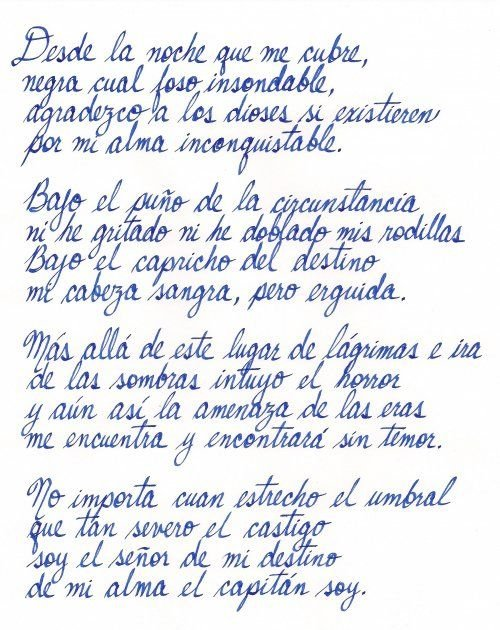
\includegraphics[width=\textwidth]{Graphics/antes_manuscrito.png}
		\caption{Facsimilar de entrada.}
		\label{fig:ocr-antes}
	\end{subfigure}
	\hfill
	\begin{subfigure}[t]{0.48\textwidth}
		\centering
		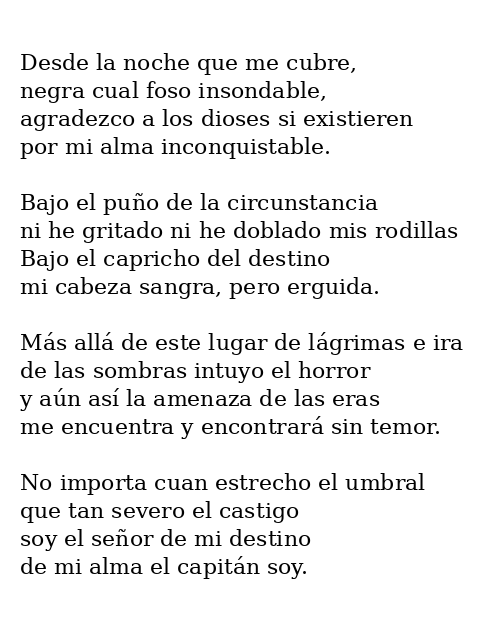
\includegraphics[width=\textwidth]{Graphics/despues_transcripcion.png}
		\caption{Transcripción producida.}
		\label{fig:ocr-despues}
	\end{subfigure}
	\caption{Comparación entre un facsimilar de entrada y la transcripción producida por un sistema OCR.}
	\label{fig:ocr-antes-despues}
\end{figure}

Cuando la imagen procede de la digitalización de un documento físico, recibe el nombre de facsimilar. Un facsimilar es una reproducción digital que preserva la apariencia visual completa del soporte: disposición de la página, tipografía, manchas, deterioro y demás características físicas. A diferencia de una transcripción, que representa únicamente el contenido textual, el facsimilar conserva la dimensión material del documento. El sistema de esta tesis opera sobre facsimilares como entrada.

El flujo de procesamiento de un sistema OCR moderno se descompone en cuatro etapas. La primera etapa es el preprocesamiento, que transforma la imagen de entrada en una representación normalizada mediante corrección de inclinación, eliminación de ruido y binarización. La segunda etapa es el análisis de diseño de página, que identifica las regiones de texto, las separa de figuras y márgenes, y detecta columnas y párrafos. La tercera etapa es el reconocimiento, durante la cual un modelo de aprendizaje automático produce la transcripción del texto de cada región o línea. La cuarta etapa es el postprocesado, que puede incluir corrección ortográfica o integración del texto en una base de datos. La figura~\ref{fig:ocr-etapas} muestra una misma imagen tras cada una de las cuatro etapas del flujo.

\begin{figure}[!htbp]
	\centering
	\begin{subfigure}[t]{0.40\textwidth}
		\centering
		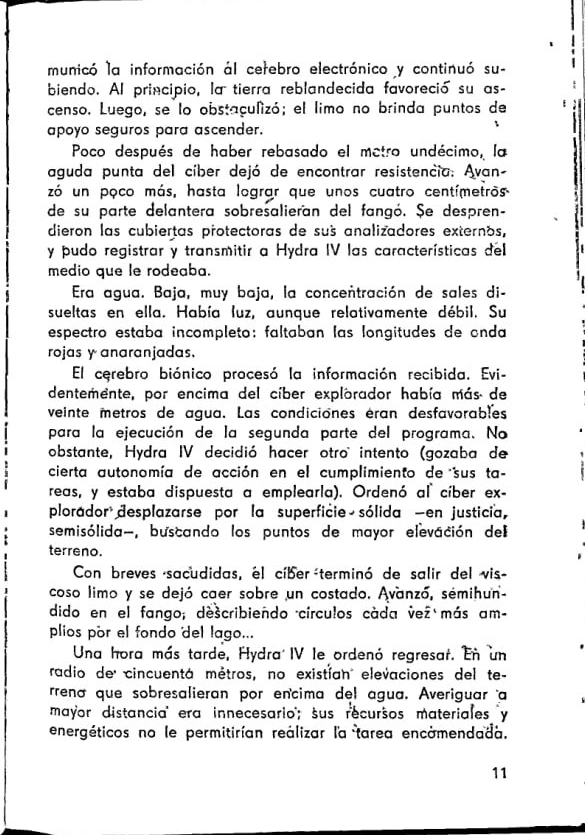
\includegraphics[width=\textwidth]{Graphics/etapa1_original.png}
		\caption{Imagen original.}
		\label{fig:etapa1}
	\end{subfigure}
	\hfill
	\begin{subfigure}[t]{0.40\textwidth}
		\centering
		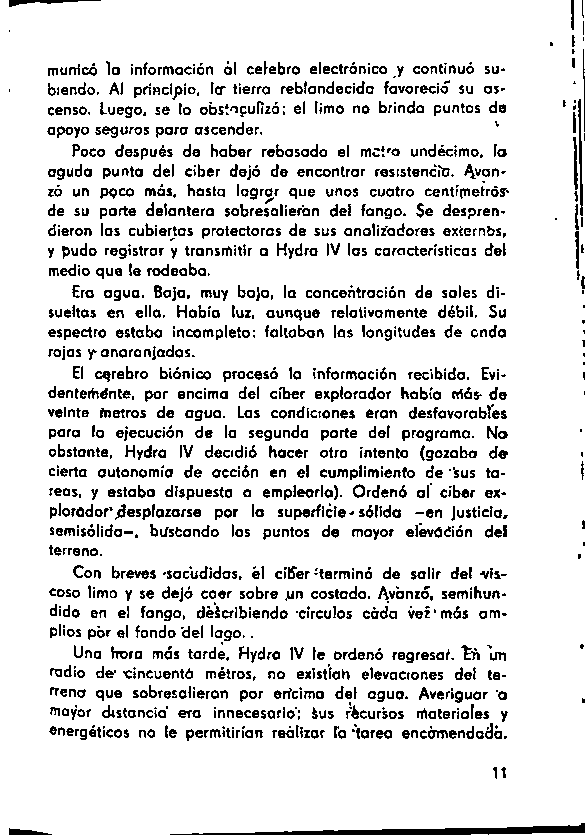
\includegraphics[width=\textwidth]{Graphics/etapa2_binarizada.png}
		\caption{Tras preprocesamiento.}
		\label{fig:etapa2}
	\end{subfigure}
	
	\vspace{0.3em}
	
	\begin{subfigure}[t]{0.40\textwidth}
		\centering
		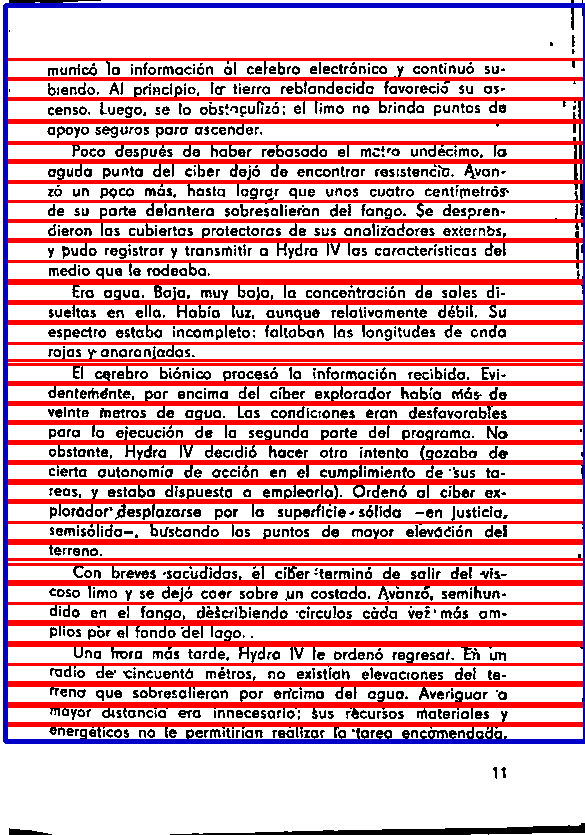
\includegraphics[width=\textwidth]{Graphics/etapa3_diseno.png}
		\caption{Tras análisis de diseño.}
		\label{fig:etapa3}
	\end{subfigure}
	\hfill
	\begin{subfigure}[t]{0.40\textwidth}
		\centering
		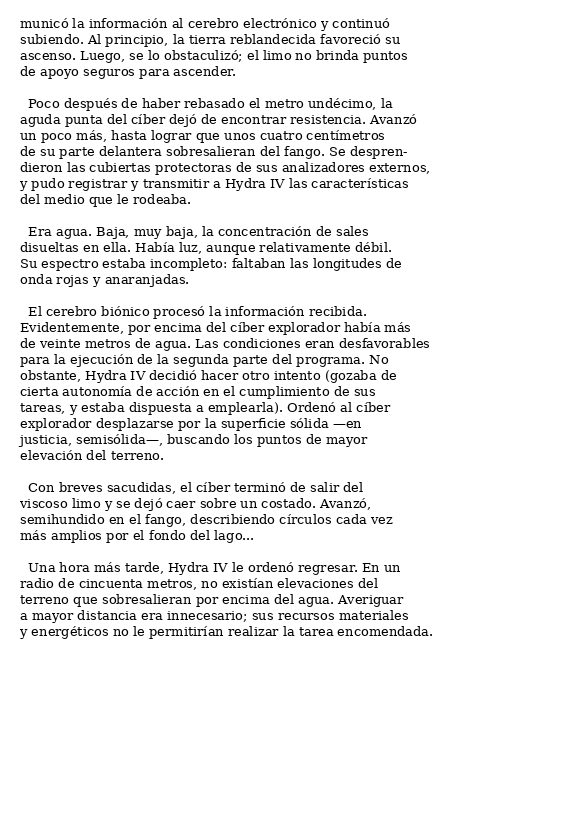
\includegraphics[width=\textwidth]{Graphics/etapa4_transcripcion.png}
		\caption{Tras reconocimiento.}
		\label{fig:etapa4}
	\end{subfigure}
	\caption{Misma página de un documento tras cada una de las cuatro etapas del flujo de procesamiento OCR.}
	\label{fig:ocr-etapas}
\end{figure}

El sistema construye las etapas de preprocesamiento y reconocimiento para documentos impresos en español. La descripción del flujo completo permite situar cada componente dentro de un marco arquitectónico de referencia. La siguiente subsección introduce dos variantes de OCR que trabajan sobre unidades de texto distintas: el OCR de caracteres aislados y el OCR de líneas completas. La decisión de cuál variante elegir determina la arquitectura que el reconocedor adopta.

\subsection{OCR de caracteres aislados frente a OCR de líneas completas}
\label{subsec:enfoques-ocr}

El enfoque clásico del OCR segmenta la imagen en caracteres individuales y clasifica cada carácter de forma independiente. El método exige que la segmentación sea perfecta. Si dos caracteres se tocan o si la separación es ambigua, el clasificador no recibe información suficiente para resolver el caso~\cite{smith2007tesseract,subramani2021survey}. Al procesar cada carácter en aislamiento, el modelo no incorpora la relación entre el carácter y sus vecinos. La consecuencia es que ciertas ambigüedades tipográficas resultan irresolubles. La secuencia ``rn'' en una fuente deteriorada, por ejemplo, puede ser visualmente indistinguible de la letra ``m'' vista en solitario, y un clasificador de caracteres aislados no posee los mecanismos para desambiguar.

El enfoque moderno toma una línea de texto completa como unidad de entrada y produce la secuencia de caracteres correspondiente en una sola pasada, sin segmentación previa. La elección justifica la arquitectura CRNN+CTC que propone Shi et al. en 2016~\cite{shi2016crnn}, que evita la segmentación explícita y aprovecha el contexto de la línea durante el reconocimiento. En el sistema para el centro de investigaciones culturales se adopta el enfoque moderno por razones que se desarrollan en el capítulo~\ref{chap:modelo}.

% -----------------------------------------------------------------------------
\section{Fundamentos de redes neuronales y aprendizaje supervisado}
\label{sec:redes-neuronales}

El sistema emplea un modelo de reconocimiento que se sustenta en redes neuronales profundas entrenadas con paradigma supervisado. La sección expone los conceptos necesarios para comprender el diseño y el funcionamiento del modelo: qué es una red neuronal artificial, en qué consiste el entrenamiento supervisado y qué es el sobreajuste.

\subsection{Redes neuronales artificiales y entrenamiento}

Una red neuronal artificial es una función paramétrica compuesta por capas de unidades de cómputo llamadas neuronas, con pesos ajustables. Cada neurona recibe una combinación lineal de las salidas de la capa anterior, aplica una función de activación no lineal y propaga el resultado a la capa siguiente. La composición de capas permite representar funciones progresivamente más abstractas de los datos de entrada~\cite{goodfellow2016deeplearning}.

El entrenamiento de la red consiste en encontrar valores de los pesos que minimizan una función de pérdida. La función mide la discrepancia entre la salida que la red produce y la salida esperada sobre un conjunto de ejemplos. La minimización opera mediante retropropagación. El algoritmo calcula el gradiente de la pérdida respecto a cada peso. A continuación, actualiza cada peso en la dirección que reduce el gradiente. El proceso itera durante múltiples pasadas sobre el \textit{corpus} de entrenamiento, y una vez concluido, los pesos condensan la información que la red extrae del \textit{corpus}. Este documento propone un sistema en el que los pesos del modelo codifican la correspondencia entre imágenes de líneas de texto y sus transcripciones.

\subsection{Aprendizaje supervisado y conjuntos de datos}

Un conjunto de datos de entrenamiento supervisado es una colección de pares en la que cada par está formado por una entrada y una etiqueta que un humano o un proceso controlado asigna~\cite{goodfellow2016deeplearning}. En el contexto del proyecto que este documento propone, cada par está formado por una imagen de una línea de texto y su transcripción exacta. El \textit{corpus} resulta supervisado porque las etiquetas resultan ciertas desde el momento en que el generador produce la imagen, lo que elimina la necesidad de anotación manual posterior.

La diversidad de los pares y la representatividad de su distribución respecto al problema real determinan la capacidad de generalización del modelo. Un \textit{corpus} reducido o sesgado produce modelos que rinden bien en el conjunto de entrenamiento pero fallan en datos nuevos. La consideración condiciona directamente las decisiones de diseño del \textit{corpus} sintético que el capítulo~\ref{chap:corpus} presenta.

\subsection{Sobreajuste y generalización}\label{subsec:sobreajuste}

El sobreajuste, conocido en la literatura como \textit{overfitting}, ocurre cuando el modelo memoriza los datos de entrenamiento en lugar de extraer patrones generalizables. Un modelo sobreajustado obtiene resultados excelentes sobre los ejemplos vistos durante el entrenamiento, pero falla en datos nuevos al no capturar los patrones subyacentes~\cite{goodfellow2016deeplearning}.

En el contexto del proyecto, el riesgo de sobreajuste se manifiesta en la selección de fuentes tipográficas para el \textit{corpus} sintético. El uso de cientos de fuentes con alta redundancia visual no aporta variabilidad efectiva pero multiplica los ejemplos con patrones equivalentes, lo cual empuja al modelo a memorizarlos~\cite{goodfellow2016deeplearning,shorten2019augmentation}. Por la misma razón se prefirió un conjunto pequeño de fuentes con diversidad estilística. Los detalles de la decisión se desarrollan en el capítulo~\ref{chap:corpus}.

% -----------------------------------------------------------------------------
\section{Propiedades estadísticas del lenguaje natural}
\label{sec:lenguaje}

El diseño del \textit{corpus} de entrenamiento descansa sobre una propiedad estadística del lenguaje natural: la distribución de frecuencias de los caracteres. En texto natural, la frecuencia de aparición de los elementos sigue una distribución de potencia~\cite{zipf1949human}. Algunos elementos concentran la mayoría de las ocurrencias, mientras que el resto resultan infrecuentes. El fenómeno se manifiesta tanto a nivel de palabras como a nivel de caracteres y sílabas.

En español, las vocales no acentuadas y unas pocas consonantes frecuentes concentran la mayor parte de las apariciones en un texto corrido. Símbolos como la raya de diálogo, las comillas angulares, los corchetes o el signo de porcentaje resultan infrecuentes en la misma medida. Un modelo que aprende sobre datos con distribución natural tenderá a reconocer correctamente las vocales y fallará en los símbolos raros por insuficiencia de ejemplos. El capítulo~\ref{chap:corpus} describe una estrategia para evitar las asimetrías por sobremuestreo. Con la propiedad estadística establecida, las siguientes secciones introducen las herramientas que miden el rendimiento del sistema y los trabajos similares que sustentan la propuesta.

% -----------------------------------------------------------------------------
\section{Métricas de evaluación de sistemas OCR}
\label{sec:metricas}

La evaluación de un sistema OCR requiere métricas que cuantifiquen la similitud entre la transcripción producida por el modelo y la transcripción de referencia. La sección define primero las métricas generales de clasificación que sustentan el vocabulario conceptual del campo, y a continuación introduce las métricas específicas del reconocimiento de secuencias.

\subsection{Precisión, recall y F1}

En clasificación, la precisión mide la proporción de predicciones positivas del modelo que resultan correctas:

\begin{equation}
	P = \frac{VP}{VP + FP},
	\label{eq:precision}
\end{equation}

donde $VP$ son los verdaderos positivos y $FP$ los falsos positivos. El \textit{recall}, llamado también sensibilidad, mide la proporción de casos positivos reales detectados por el modelo:

\begin{equation}
	R = \frac{VP}{VP + FN},
	\label{eq:recall}
\end{equation}

donde $FN$ son los falsos negativos. La medida F1 es la media armónica de precisión y recall, y combina ambas en un solo número:

\begin{equation}
	F_1 = \frac{2 \cdot P \cdot R}{P + R}.
	\label{eq:f1}
\end{equation}

Existe una compensación inherente entre precisión y recall. Un modelo restrictivo alcanza alta precisión a costa de un recall bajo. Un modelo permisivo presenta el comportamiento opuesto. La F1 equilibra ambos extremos y resulta útil cuando el problema demanda una métrica única. Las tres definiciones no resultan directamente aplicables al OCR de secuencias, pero constituyen el vocabulario conceptual sobre el cual el campo construye sus métricas específicas.

\subsection{Tasa de error de carácter, tasa de error de palabra y exactitud por línea}

La tasa de error de carácter, conocida por sus siglas inglesas CER, del término \textit{Character Error Rate}~\cite{jurafsky2024slp}, mide la proporción de caracteres incorrectos en la transcripción respecto a la transcripción de referencia. Se calcula mediante la distancia de Levenshtein a nivel de carácter, normalizada por la longitud de la referencia:

\begin{equation}
	CER = \frac{S_c + I_c + D_c}{N_c},
	\label{eq:cer}
\end{equation}

donde $S_c$, $I_c$ y $D_c$ son los números de sustituciones, inserciones y eliminaciones de caracteres, y $N_c$ es el número total de caracteres de la referencia. La métrica satisface $0 \leq \mathrm{CER} \leq 1$, donde un CER de~0 corresponde a una transcripción perfecta y un CER de~1 indica un número de errores igual al número de caracteres del texto de referencia.

La tasa de error de palabra, denominada WER, del término \textit{Word Error Rate}~\cite{jurafsky2024slp}, es análoga al CER pero a nivel de palabras:

\begin{equation}
	WER = \frac{S_w + I_w + D_w}{N_w}.
	\label{eq:wer}
\end{equation}

El WER es más exigente que el CER porque un solo carácter incorrecto dentro de una palabra cuenta como un error de palabra completo. La diferencia hace al WER sensible a errores que distorsionan el significado léxico, y menos informativo sobre errores aislados en caracteres especiales.

La exactitud por línea~\cite{jurafsky2024slp} es la métrica más exigente de las tres. Mide la proporción de líneas de texto donde la transcripción coincide exactamente con la referencia, sin ningún error:

\begin{equation}
	\mathrm{LineAcc} = \frac{\text{líneas sin error}}{\text{total de líneas}}.
	\label{eq:lineacc}
\end{equation}

Una sola sustitución en cualquier posición de la línea la marca como incorrecta. La métrica resulta útil para evaluar la viabilidad del sistema en casos de uso donde no se admite intervención humana posterior. Las tres métricas, tomadas en conjunto, ofrecen una visión complementaria del rendimiento. El CER informa sobre la tasa de error tipográfico, el WER sobre la integridad léxica y la exactitud por línea sobre la viabilidad para automatización completa. Con el vocabulario de evaluación definido, la siguiente sección revisa los trabajos previos que abordan problemas equivalentes al planteado en la tesis.

% -----------------------------------------------------------------------------
\section{Estado del arte}
\label{sec:estado-arte}

Esta sección sintetiza los trabajos previos sobre los que se apoya el desarrollo del sistema. La revisión se organiza por bloques temáticos. El primero presenta los motores OCR clásicos de código abierto. El segundo aborda las arquitecturas basadas en aprendizaje profundo con función de pérdida \textit{Connectionist Temporal Classification}, conocida por sus siglas inglesas CTC~\cite{graves2006ctc}. El tercero recoge las propuestas basadas en \textit{transformers}~\cite{vaswani2017transformer}. El cuarto trata la generación sintética de datos para OCR. El quinto introduce las plataformas de digitalización documental de uso institucional. El sexto cierra con los trabajos específicos para texto impreso en español.

\subsection{Motores OCR clásicos: Tesseract y Calamari}

Tesseract es un motor OCR de código abierto, distribuido bajo licencia Apache~2.0. Lo desarrolló originalmente Hewlett-Packard entre los años ochenta y noventa, y entre 2006 y agosto de 2017 lo mantuvo Google~\cite{smith2007tesseract}. Desde esa fecha el desarrollo lo continúa la comunidad de código abierto a través del repositorio público del proyecto. El motor admite más de~100 idiomas y dispone de paquetes de datos entrenados para el reconocimiento. A partir de su versión~4, el reconocedor interno de Tesseract es una red neuronal basada en LSTM. La arquitectura sitúa al motor en la familia de las soluciones con función de pérdida CTC~\cite{graves2006ctc}.

Calamari, presentado por Wick et al.~\cite{wick2018calamari}, es un motor OCR de código abierto especializado en el reconocimiento de líneas de texto, con énfasis en documentos impresos históricos. La arquitectura central de Calamari combina una red convolucional~\cite{goodfellow2016deeplearning} con una red recurrente bidireccional~\cite{goodfellow2016deeplearning} y una capa CTC, esquema equivalente al de la CRNN~\cite{shi2016crnn}. El motor ha alcanzado popularidad en el ámbito de las humanidades digitales por su capacidad para procesar tipografías históricas como la \textit{Fraktur}~\cite{breuel2013ocropus}.

Ambos motores ofrecen reconocimiento listo para uso, pero presentan limitaciones para el problema que motiva a esta tesis. Tesseract dispone de un modelo para el español de propósito general, sin adaptación a la distribución de caracteres ni al perfil tipográfico de un dominio documental específico. Calamari requiere conjuntos de datos con anotación humana específicos para cada dominio. En el capítulo~\ref{chap:corpus} se ofrece una justificación a detalle de la decisión de desarrollar un \textit{corpus} propio.

\subsection{Arquitecturas basadas en aprendizaje profundo: CRNN + CTC}
\label{subsec:crnn-ctc-arte}

El trabajo de Shi, Bai y Yao~\cite{shi2016crnn} propuso en~2016 la arquitectura CRNN, que combina una red neuronal convolucional con una red neuronal recurrente bidireccional, y que la función de pérdida \textit{Connectionist Temporal Classification}, CTC por sus siglas en inglés, entrena. La arquitectura transcribe líneas de texto completas sin segmentación previa de caracteres, y como describe la sección~\ref{subsec:enfoques-ocr}, esta propiedad la sitúa en el enfoque moderno. Graves et al.~\cite{graves2006ctc} introdujeron por primera vez la función CTC para el reconocimiento de habla, y permite entrenar redes que producen secuencias de longitud variable sin alineamiento explícito entre entrada y salida.

El trabajo de Breuel et al.~\cite{breuel2013ocropus} demostró en~2013 que una red bidireccional LSTM, sin modelo de lenguaje ni postprocesado, alcanza tasas de error inferiores al~2\,\% sobre texto impreso en inglés y sobre Fraktur degradada artificialmente. El resultado estableció la viabilidad de las arquitecturas LSTM para el reconocimiento de líneas impresas, y abrió la puerta al entrenamiento sobre \textit{corpus} con artefactos sintéticos que reproducen las condiciones visuales de los documentos objetivo.

La arquitectura CRNN+CTC presenta dos propiedades que la convierten en la opción preferida para el sistema. Primero, permite explotar el contexto oracional durante el reconocimiento, lo cual desambigua errores tipográficos que un clasificador de caracteres aislados no puede resolver. Segundo, su entrenamiento sobre líneas completas se ajusta al formato del \textit{corpus} sintético generado. Las decisiones de diseño del modelo concreto se exponen en el capítulo~\ref{chap:modelo}.

\subsection{Arquitecturas basadas en transformers: TrOCR y derivados}

A partir de la introducción de la arquitectura \textit{Transformer} por Vaswani et al.~\cite{vaswani2017transformer} en~2017, el aprendizaje profundo aplicado a tareas de lenguaje y visión adoptó el mecanismo de atención de forma generalizada. En el campo del reconocimiento óptico de caracteres, el trabajo de Li et al.~\cite{li2021trocr} propuso en~2021 la arquitectura TrOCR, que reemplaza por completo el esquema CNN+RNN. Como codificador de imagen emplea un \textit{Vision Transformer}, y como decodificador un \textit{transformer} de texto. El modelo se entrena con un esquema de preentrenamiento sobre datos sintéticos seguido de \textit{fine-tuning} sobre datos reales.

El trabajo de Laurent y Lauar~\cite{laurent2024spanishtrocr} adaptó TrOCR al español mediante \textit{fine-tuning} desde el punto de control en inglés. El trabajo concluye que el \textit{fine-tuning} desde un modelo en inglés produce mejores resultados que el entrenamiento de un decodificador específico para el español. La estrategia exige infraestructura computacional mayor que la CRNN+CTC para alcanzar mejoras marginales sobre tipografías de imprenta estándar, donde la arquitectura CRNN ya rinde por debajo del~2\,\% de CER. La consideración sustenta la elección de CRNN+CTC para el sistema descrito en la tesis, justificada en detalle en el capítulo~\ref{chap:modelo}.

\subsection{Generación sintética de datos para OCR}

El trabajo de Jaderberg et al.~\cite{jaderberg2014synthetic} demostró en~2014 que el entrenamiento de redes neuronales sobre datos sintéticos puede sustituir el uso de datos reales en escenarios de reconocimiento de texto natural. Los modelos resultantes alcanzan tasas de error competitivas con \textit{corpus} generados enteramente por procesos automáticos. La demostración estableció la generación sintética como una alternativa viable cuando los datos con anotación humana son escasos o inexistentes para el idioma objetivo.

Trabajos posteriores extendieron la idea a configuraciones específicas. Etter et al.~\cite{etter2019synthrecipe} describieron un protocolo de generación sintética para sistemas OCR de líneas completas, con énfasis en la diversidad tipográfica y en los artefactos del escaneo real. La línea de trabajo más cercana al proyecto que esta tesis describe es la de Laurent y Lauar~\cite{laurent2024spanishtrocr}, que generó un \textit{corpus} de dos millones de muestras para entrenar TrOCR en español a partir de páginas web de la Wikipedia hispanoamericana.

El sistema que esta tesis presenta entrena con datos que el procedimiento produce de manera similar a la que el estado del arte describe, con dos diferencias al respecto. Primero, el generador toma el \textit{corpus} de obras literarias del dominio público en lugar de texto extraído de la web. La elección asegura riqueza léxica y densidad de signos tipográficos propios del español formal. Segundo, una estrategia explícita de sobremuestreo por grupos equilibra las frecuencias de caracteres, en lugar de una distribución uniforme o de la distribución natural del \textit{corpus} base. El capítulo~\ref{chap:corpus} desarrolla la justificación de ambas decisiones.

\subsection{Plataformas de digitalización documental: Transkribus}

Muehlberger et al.~\cite{muehlberger2019transkribus} describen Transkribus, plataforma para el reconocimiento, transcripción y búsqueda de documentos históricos. La cooperativa READ-COOP mantiene la plataforma actualmente, desarrollada en el marco del proyecto europeo \textit{Recognition and Enrichment of Archival Documents}, conocido por sus siglas READ. La plataforma integra motores de reconocimiento de texto manuscrito y OCR para impresos junto con herramientas de gestión, búsqueda y revisión colaborativa de transcripciones. Cuenta con una comunidad consolidada de decenas de miles de usuarios registrados.

Transkribus constituye la referencia funcional más cercana al sistema que este trabajo aspira a desarrollar. Integra el flujo completo, desde la subida del facsimilar hasta la corrección de la transcripción mediante un editor colaborativo. El capítulo~\ref{chap:web} presenta una aplicación que adopta un esquema funcional similar a Transkribus, adaptado al contexto del Instituto Juan Marinello y a la integración de modelos OCR para el idioma español.

\subsection{Trabajos previos sobre OCR para texto impreso en español}

La literatura específica sobre OCR para texto impreso en español es escasa. La mayor parte de los recursos disponibles asumen el idioma inglés y, en menor medida, otros idiomas con presencia mayoritaria en los conjuntos de datos públicos~\cite{laurent2024spanishtrocr}. El conjunto de competiciones internacionales \textit{Robust Reading Competition on Multi-lingual Scene Text} de ICDAR~\cite{nayef2019icdarmlt}, referencia metodológica del campo, contempla diez lenguas en su edición de~2019: el chino, el japonés, el coreano, el inglés, el francés, el árabe, el italiano, el alemán, el bangla y el devanagari. La ausencia del español del conjunto es ilustrativa del estado del arte en el campo. El trabajo de Laurent y Lauar~\cite{laurent2024spanishtrocr} constituye una de las primeras propuestas dedicadas explícitamente al español, y limita su evaluación a documentos del tipo \textit{Visual Rich Document}~\cite{laurent2024spanishtrocr}, con presencia frecuente de formularios y campos estructurados.


Los \textit{datasets} de uso común en investigación OCR omiten signos frecuentes en documentos formales en español. Entre los signos ausentes están la raya de diálogo, las comillas angulares, los signos de apertura de interrogación y exclamación, la eñe y las vocales acentuadas. Un modelo que aprende sobre vocabularios incompletos resulta incapaz de transcribir correctamente los documentos formales en español que motivan el trabajo. El capítulo~\ref{chap:corpus} presenta el análisis sistemático de los \textit{datasets} existentes, junto con la justificación del desarrollo de un \textit{corpus} propio.


% -----------------------------------------------------------------------------
\section{Tecnologías para el desarrollo de la aplicación web}
\label{sec:tecnologias-web}

Para comodidad del usuario final, el desarrollo de esta tesis incorpora una aplicación web que el capítulo~\ref{chap:web} describe. Esta aplicación, que permite usar las funcionalidades del sistema de manera fácil, descansa sobre un conjunto de tecnologías abiertas que proyectos similares emplean ampliamente. La sección introduce el \textit{framework} de desarrollo y los mecanismos de persistencia. La descripción detallada de las decisiones de arquitectura espera al capítulo correspondiente.

\subsection{Django y el patrón Modelo-Vista-Plantilla}\label{subsec:django-mvt}

Django es un \textit{framework} de desarrollo web en Python, distribuido bajo licencia BSD~\cite{osi-bsd}. Está diseñado en torno al patrón Modelo-Vista-Plantilla, conocido por sus siglas MVT, del término inglés \textit{Model-View-Template}~\cite{django-mvt}. El patrón separa la lógica de los datos en los modelos, la lógica de presentación en las plantillas, y la lógica de control en las vistas. La separación facilita el mantenimiento del código y la división del trabajo entre componentes. La figura~\ref{fig:mvt-diagrama} resume las relaciones entre los cuatro elementos del patrón.

\begin{figure}[!htbp]
	\centering
	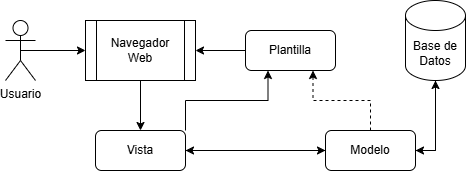
\includegraphics[width=0.78\textwidth]{Graphics/mvt_diagrama.png}
	\caption{Patrón Modelo-Vista-Plantilla de Django. El navegador del usuario envía una petición a la vista, que consulta el modelo cuando necesita datos persistentes; el modelo intermedia con la base de datos. La vista pasa los datos a la plantilla, que produce la respuesta HTML que el navegador recibe.}
	\label{fig:mvt-diagrama}
\end{figure}

Django ofrece una infraestructura integrada de correspondencia objeto-relacional, conocida por sus siglas ORM del término inglés \textit{Object-Relational Mapping}, un sistema de migraciones automatizado, un mecanismo declarativo de formularios y una infraestructura de autenticación con roles y permisos. La combinación reduce la cantidad de código necesario para implementar las funcionalidades comunes de una aplicación web. El esfuerzo de desarrollo se concentra entonces en los componentes específicos del problema, como la integración del modelo de OCR y el editor de doble panel para la revisión de transcripciones.

\subsection{Persistencia: PostgreSQL y XML}

La aplicación utiliza dos mecanismos de persistencia complementarios. Los metadatos estructurados de los documentos se almacenan en una base de datos relacional PostgreSQL~\cite{postgresql}. Las transcripciones, que combinan texto plano con regiones definidas por el usuario y referencias a páginas, se almacenan en ficheros XML, uno por cada página.

La decisión responde a dos consideraciones. La primera es la legibilidad humana directa. Un revisor puede abrir el fichero XML con un editor de texto e interpretar y modificar la transcripción sin herramientas auxiliares. La segunda es la posibilidad de convertir las transcripciones a estándares mayores como ALTO~\cite{loc-alto}, PAGE-XML~\cite{pletschacher2010page} o TEI~\cite{tei-consortium}, en caso de que el archivo se integre en un repositorio institucional con requisitos de interoperabilidad. El esquema que el trabajo emplea constituye un subconjunto razonable de ALTO, lo que facilita la migración futura sin retrabajo. El capítulo~\ref{chap:web} describe a detalle el esquema y el modelo de datos relacional que el sistema utiliza.

% -----------------------------------------------------------------------------
% Transición al capítulo 2
% -----------------------------------------------------------------------------

Con la fundamentación teórica establecida, los antecedentes presentados y la metodología declarada, el capítulo cierra. El capítulo siguiente aborda la primera contribución técnica del trabajo: la generación del \textit{corpus} sintético de pares imagen--transcripción sobre el que se entrena el modelo de reconocimiento.

	% Numeración del capítulo: 2.
\setcounter{chapter}{1}

\chapter{Generación del \textit{corpus} sintético}\label{chap:corpus}

El presente capítulo describe el primer componente técnico del sistema: la construcción del \textit{corpus} de pares imagen--transcripción que entrena el modelo de reconocimiento. El capítulo se organiza en cinco secciones. La sección~\ref{sec:justificacion-corpus} justifica la decisión de generar un \textit{corpus} propio en lugar de utilizar uno público. La sección~\ref{sec:diseno-corpus} expone las tres decisiones de diseño que estructuran el \textit{corpus}: la estrategia de sobremuestreo, el \textit{corpus} textual base y la selección tipográfica. La sección~\ref{sec:implementacion-generador} describe la implementación del generador, desde la construcción de las cadenas de texto hasta el renderizado y la simulación de degradación visual. La sección~\ref{sec:vocabulario} presenta el vocabulario indexado del sistema. La sección~\ref{sec:eda-corpus} reporta el análisis exploratorio del \textit{corpus}.

% -----------------------------------------------------------------------------
\section{Justificación de la generación de un \textit{corpus} propio}
\label{sec:justificacion-corpus}

La generación de un \textit{corpus} de entrenamiento desde cero conlleva un coste elevado en diseño, implementación y validación. La decisión solo se justifica cuando las alternativas disponibles presentan limitaciones que las hacen inadecuadas para el problema. La sección presenta el análisis de los \textit{datasets} públicos para reconocimiento óptico de caracteres~\cite{mori1992hocr} en español y motiva, a partir de la detección de limitaciones, a la construcción de un \textit{corpus} propio. A continuación, la sección introduce el desbalance de clases inherente al lenguaje natural, que condiciona el diseño del \textit{corpus}.

\subsection{Análisis y descarte de datasets existentes para OCR en español}
\label{subsec:descarte-datasets}

Antes de construir el \textit{corpus} propio, el trabajo evaluó los \textit{datasets} públicos disponibles para OCR en español. La evaluación identificó cuatro limitaciones que los descartan como base de entrenamiento para el sistema. A las cuatro limitaciones se añade una restricción adicional de disponibilidad: la cantidad de recursos para texto impreso en español es mucho menor que para idiomas con presencia mayoritaria en investigación OCR como el inglés, según documenta el trabajo de Laurent y Lauar~\cite{laurent2024spanishtrocr}.

La primera limitación es la cobertura incompleta de caracteres. Los \textit{datasets} omiten signos frecuentes en documentos formales en español, entre ellos la raya de diálogo, las comillas angulares, los signos de apertura de interrogación y exclamación, la eñe y las vocales con tilde. Un modelo cuyo vocabulario omite alguno de estos signos no puede transcribir correctamente los documentos que motivan el trabajo.

La segunda limitación es la redundancia tipográfica. Sus creadores generaron varios de los \textit{datasets} con cientos de fuentes visualmente similares, lo que multiplica los ejemplos con patrones equivalentes y favorece el sobreajuste sin aportar variabilidad efectiva~\cite{goodfellow2016deeplearning}. La sección~\ref{subsec:sobreajuste} del capítulo anterior introdujo la consideración y discutió el riesgo del sobreajuste asociado a la redundancia visual.

La tercera limitación es la inviabilidad de corregir las dos primeras mediante augmentación posterior. Corregir la cobertura incompleta exigiría descargar y gestionar un número equivalente de fuentes para los símbolos ausentes. Corregir la redundancia tipográfica exigiría descartar manualmente fuentes similares hasta dejar un subconjunto representativo. La combinación de las dos correcciones tiene un coste manual elevado y no garantiza equilibrio en el \textit{corpus}.

La cuarta limitación es la ausencia de contexto léxico. Los \textit{datasets} contienen únicamente imágenes de caracteres aislados, lo que impide que el modelo aproveche el contexto oracional durante el reconocimiento. El formato aislado es incompatible con la arquitectura CRNN~\cite{shi2016crnn} con función de pérdida CTC~\cite{graves2006ctc} que el sistema adopta, que opera sobre líneas de texto completas según describió la sección~\ref{subsec:crnn-ctc-arte} del capítulo anterior.

La cuarta limitación admite una contraposición aparente: si los recursos disponibles operan sobre caracteres aislados, una alternativa consistiría en adaptar el sistema a una arquitectura clásica de reconocimiento por carácter. El trabajo descarta la opción por la diferencia de rendimiento que el estado del arte documenta. Las arquitecturas que clasifican caracteres aislados ignoran el contexto oracional y producen errores irresolubles ante ambigüedades tipográficas, según argumentó la sección~\ref{subsec:enfoques-ocr} del capítulo anterior. La elección de la arquitectura CRNN+CTC, bajo el sustento de sus ventajas (sección~\ref{subsec:crnn-ctc-arte}), fija las propiedades del \textit{corpus} que el modelo necesita. Las limitaciones de los recursos disponibles motivan, por tanto, la generación de un \textit{corpus} adecuado a la arquitectura, no la sustitución de la arquitectura por una compatible con los recursos disponibles.

Las cuatro limitaciones, junto a la escasez documentada de \textit{datasets} en español y a la inviabilidad de adaptar la arquitectura, justifican la generación de un \textit{corpus} propio adaptado al problema.

\subsection{Desbalance de clases en el contexto del español}
\label{subsec:desbalance}

El desbalance de clases ocurre cuando algunas clases tienen muchas más muestras que otras en el \textit{corpus} de entrenamiento. La presencia del desbalance lleva al modelo a optimizar el rendimiento sobre las clases mayoritarias a expensas de las minoritarias, porque la pérdida global cae más al mejorar el reconocimiento de las clases con mayor representación~\cite{buda2018imbalance}. En el contexto del OCR para español, donde las clases son los caracteres, la ley de Zipf~\cite{zipf1949human}, que la sección~\ref{sec:lenguaje} del capítulo anterior describió previamente, provoca que las vocales y las consonantes frecuentes tengan más apariciones que símbolos como la raya de diálogo, las comillas angulares o el signo de porcentaje.

Sin corrección, el modelo que aprende sobre una distribución natural reconoce con precisión las vocales y falla en los símbolos raros por insuficiencia de ejemplos. La solución no consiste en alterar la naturaleza estadística del lenguaje sino en incrementar la frecuencia con que los símbolos raros aparecen en el \textit{corpus} de entrenamiento. La siguiente sección describe el procedimiento concreto, que la literatura denomina sobremuestreo de clases minoritarias~\cite{chawla2002smote}.

% -----------------------------------------------------------------------------
\section{Diseño del \textit{corpus}}
\label{sec:diseno-corpus}

Tres decisiones de diseño independientes definen la construcción del \textit{corpus}. La primera fija la estrategia de sobremuestreo que ataca a los caracteres minoritarios. La segunda fija el origen del texto que el generador renderiza en las imágenes. La tercera fija las fuentes tipográficas con que el generador renderiza. Las siguientes subsecciones desarrollan las tres decisiones.

\subsection{Estrategia de sobremuestreo: grupos A, B y C}
\label{subsec:sobremuestreo}

El sobremuestreo de clases minoritarias incrementa de forma deliberada la frecuencia de los caracteres subrepresentados en el \textit{corpus} de entrenamiento. En este proyecto, el sistema implementa el procedimiento mediante una estrategia de tres niveles que opera sobre la distribución de frecuencias objetivo del generador. El diseño reparte los caracteres en tres grupos según el factor de sobremuestreo que reciben, que la tabla~\ref{tab:grupos-sobremuestreo} resume.

\begin{table}[!htbp]
	\centering
	\caption{Grupos de sobremuestreo del \textit{corpus} sintético.}
	\label{tab:grupos-sobremuestreo}
	\begin{tabular}{lp{8.5cm}c}
		\toprule
		\textbf{Grupo} & \textbf{Caracteres} & \textbf{Factor} \\
		\midrule
		A & Vocales no acentuadas (a, e, i, o, u) y consonantes frecuentes (s, r, n, l, d, t, c, m, p). Distribución próxima a la observada en el \textit{corpus} textual base. & $\times 1$ \\
		\addlinespace
		B & Vocales con tilde (á, é, í, ó, ú), ñ, consonantes medias, y todas las letras mayúsculas. & $\times 2$ a $\times 12$ \\
		\addlinespace
		C & Consonantes raras (k, w, x, j) y signos tipográficos específicos del español formal (—, «, », \%, \&, \$, \#, [, ]). & $\times 10$ a $\times 500$ \\
		\bottomrule
	\end{tabular}
\end{table}

El grupo A mantiene la distribución naturalista del español como línea base. El sistema calibra esta distribución sobre las frecuencias de caracteres del \textit{corpus} textual de origen, que la subsección~\ref{subsec:gutenberg} describe. La elección permite al modelo aprender el ritmo léxico real del idioma. Los grupos B y C incrementan la frecuencia de los caracteres subrepresentados hasta que cada símbolo supera un umbral mínimo de 500 apariciones en el \textit{corpus}.

Dos propiedades de la arquitectura que el trabajo adopta sustentan la elección del umbral en 500 apariciones. La primera es que la arquitectura CRNN+CTC no aprende cada carácter como una clase independiente. Las capas convolucionales tempranas extraen rasgos visuales que múltiples caracteres comparten, como bordes, curvas y uniones. La detección de un rasgo en cualquier carácter contribuye al aprendizaje del rasgo en todos los caracteres que lo comparten. La transferencia interna de representaciones reduce el número de muestras independientes que cada clase necesita respecto al que requeriría un clasificador sin compartición. La segunda propiedad es la augmentación de datos que el sistema aplica en línea durante el entrenamiento (capítulo~\ref{chap:modelo}). La augmentación consiste en aplicar transformaciones aleatorias a cada imagen del \textit{corpus} en cada época, lo que produce muestras visualmente distintas a partir de los mismos pares imagen--transcripción que el disco almacena. La literatura documenta la técnica como uno de los mecanismos de regularización más efectivos para problemas de visión con datos limitados, según el estudio sistemático de Shorten y Khoshgoftaar~\cite{shorten2019augmentation}. El sistema presenta al modelo cada aparición de un carácter en el \textit{corpus} en múltiples variantes a lo largo del entrenamiento, gracias a transformaciones que afectan al ancho de trazo, a la perspectiva, al contraste y al ruido aditivo. La consecuencia es que el número efectivo de exposiciones a cada símbolo es mucho mayor que el recuento directo de apariciones en el \textit{corpus}, lo que sustenta la elección del umbral de 500. El capítulo~\ref{chap:modelo} ofrece el argumento detallado sobre la augmentación durante el entrenamiento.

El diseño no constituye una distorsión arbitraria de los datos sino una solución al problema del desbalance. El grupo A preserva la distribución real del español, los grupos B y C compensan la escasez estadística de símbolos que el sistema debe igualmente aprender a reconocer. Definida la estrategia de balance, la siguiente decisión concierne al texto que el generador renderiza en las imágenes.

\subsection{Corpus textual: Project Gutenberg}
\label{subsec:gutenberg}

El generador extrae el texto de las imágenes de obras literarias en español del dominio público disponibles en Project Gutenberg~\cite{gutenberg}, una biblioteca digital que ofrece textos del dominio público de forma gratuita. Dos propiedades del registro literario sustentan la elección de obras literarias clásicas.

La primera propiedad es la riqueza léxica. El vocabulario de la literatura clásica es amplio y variado, lo que asegura que el modelo aprende a reconocer una diversidad de palabras y no se especializa en un subconjunto léxico propio de un único género o registro.

La segunda propiedad es la alta densidad de signos tipográficos del español formal. El texto literario emplea con frecuencia la raya de diálogo, las comillas angulares, los signos de apertura de interrogación y exclamación, y las vocales con tilde. La ausencia de estos signos en los datasets motiva su descarte para el entrenamiento, como explicó la subsección~\ref{subsec:descarte-datasets}.

Las dos propiedades contribuyen directamente a la construcción de un \textit{corpus} específico para el objetivo del sistema. La siguiente sección aborda la decisión de diseño que concierne a las fuentes tipográficas con que el generador renderiza el texto.

\subsection{Selección tipográfica para el \textit{corpus} de entrenamiento}
\label{subsec:fuentes-entrenamiento}

El generador renderiza el \textit{corpus} de entrenamiento con nueve fuentes tipográficas. El trabajo eligió el número de forma deliberada por dos razones. Primero, un número reducido de fuentes con diversidad estilística sustantiva resulta preferible a centenares de fuentes con redundancia visual elevada, según argumentó la subsección~\ref{subsec:descarte-datasets}. Segundo, la selección de fuentes cubre tres familias estilísticas: monoespacios, serif clásicas y simulaciones de máquina de escribir.

La tabla~\ref{tab:fuentes-entrenamiento} enumera las fuentes incluidas en el \textit{corpus} de entrenamiento y la familia estilística a la que pertenece cada una.

\begin{table}[!htbp]
	\centering
	\caption{Fuentes tipográficas del \textit{corpus} de entrenamiento.}
	\label{tab:fuentes-entrenamiento}
	\begin{tabular}{lll}
		\toprule
		\textbf{Familia estilística} & \textbf{Fuente} & \textbf{Cantidad} \\
		\midrule
		Monoespacio & CourierPrime, CutiveMono, Inconsolata, & 5 \\
		& JetBrainsMono, RobotoMono & \\
		\addlinespace
		Serif clásica & CrimsonPro, EBGaramond, LibreBaskerville & 3 \\
		\addlinespace
		Máquina de escribir & SpecialElite & 1 \\
		\bottomrule
	\end{tabular}
\end{table}

Los cinco monoespacios comparten la propiedad de que cada carácter ocupa el mismo ancho, lo que produce un patrón visual distinto al de las tipografías proporcionales. Las tres serif clásicas presentan remates en los extremos de los trazos. La fuente SpecialElite imita la apariencia de las máquinas de escribir, con irregularidades de trazo y leves desalineaciones entre caracteres. Las tres familias cubren registros visuales que aparecen con frecuencia en los documentos del acervo objetivo: documentos mecanografiados, textos impresos en imprenta tradicional y documentos técnicos compuestos con tipografías monoespacio.

La selección no agota la variabilidad tipográfica de los documentos reales en español. Una etapa posterior de adaptación del modelo aborda la cobertura adicional sobre tipografías serif modernas, que el capítulo~\ref{chap:modelo} describe.

% -----------------------------------------------------------------------------
\section{Implementación del generador}
\label{sec:implementacion-generador}

La implementación del generador se divide en tres bloques funcionales. El primero produce cadenas de texto cuya distribución agregada de caracteres se ajusta a las frecuencias objetivo. El segundo renderiza cada cadena como una imagen de línea con la fuente correspondiente. El tercero simula las condiciones de degradación visual que aparecen en documentos digitalizados. Las siguientes subsecciones describen los tres bloques.

\subsection{Generación de cadenas balanceadas}
\label{subsec:cadenas-balanceadas}

El generador parte de los textos descargados de Project Gutenberg~\cite{gutenberg}. La tokenización opera mediante la expresión regular:
\begin{center}
	\verb![a-zA-ZáéíóúÁÉÍÓÚüÜñÑ]+|\d|[—«»]|[^\w\s]!
\end{center}
que identifica cuatro categorías de \textit{tokens}: palabras alfabéticas del español, dígitos aislados, signos tipográficos específicos del español como la raya de diálogo o las comillas angulares, y signos de puntuación restantes. La elección de tratar la raya y las comillas angulares como \textit{tokens} independientes, en lugar de incluirlas en la clase general de puntuación, garantiza la representación explícita de los símbolos del grupo C que la subsección~\ref{subsec:sobremuestreo} define.

El conjunto de \textit{tokens} únicos se indexa por carácter. La estructura resultante asocia a cada carácter del vocabulario la lista de \textit{tokens} que lo contienen. La indexación permite, dado un carácter deficitario, seleccionar de forma directa un \textit{token} que lo contenga y compensar la subrepresentación del carácter en el \textit{corpus}.

El algoritmo de generación construye cada cadena mediante el procedimiento siguiente. Sortea un número aleatorio de \textit{tokens} entre cinco y quince. Sortea una longitud máxima de cadena entre veinticinco y setenta y cinco caracteres, con distribución uniforme. El sorteo de la longitud máxima evita que las cadenas se concentren cerca del límite superior y reproduce el rango de longitudes que aparecen en líneas de texto reales. A continuación calcula, para cada carácter del vocabulario, el déficit respecto a la frecuencia objetivo en el \textit{corpus} generado hasta el momento. El cálculo emplea la expresión:

\begin{equation}
	\delta(c) = \frac{p(c)}{P} \cdot N - n(c),
	\label{eq:deficit}
\end{equation}

donde $p(c)$ es el peso objetivo del carácter $c$, $P$ es la suma de los pesos objetivo, $N$ es el número total de caracteres ya generados y $n(c)$ es el número de apariciones de $c$ hasta el momento. Un déficit positivo indica que el carácter aparece menos de lo previsto por la distribución objetivo. Un déficit negativo indica que aparece más de lo previsto.

Para cada \textit{token} de la cadena, el algoritmo ordena los caracteres por déficit descendente. Mezcla aleatoriamente los quince primeros y selecciona el primero con déficit positivo cuya lista de \textit{tokens} asociados no esté vacía. Elige al azar un \textit{token} de la lista. La estrategia introduce aleatoriedad sobre los caracteres más necesarios y evita producir cadenas mecánicas dominadas siempre por un único carácter deficitario. Si ningún carácter prioritario satisface las condiciones, el algoritmo elige un \textit{token} aleatorio del \textit{corpus} completo.

A modo de ejemplo supóngase que, tras generar un número apreciable de cadenas, el contador global presenta déficit positivo para `ñ', `«' y `—', y déficit negativo para `e' y `a' (caracteres frecuentes ya sobrerrepresentados). Cuando el algoritmo construye la siguiente cadena, los tres caracteres con déficit positivo aparecen entre los primeros quince del ordenamiento. Tras el barajado de esos quince, el algoritmo selecciona el primero cuya lista de \textit{tokens} asociados no esté vacía y muestrea de ella. Si la `ñ' resulta primera, el muestreo escoge un \textit{token} aleatorio del subconjunto que contiene `ñ' --- por ejemplo, ``mañana'', ``señor'' o ``año''---, y lo concatena con los demás \textit{tokens} ya elegidos. La cadena resultante podría ser ``mañana —dijo el señor«''. La iteración sobre el contador global compensa de forma progresiva el déficit que se va acumulando sobre cada carácter raro.

El algoritmo construye la cadena resultante al concatenar los \textit{tokens} con espacios entre ellos. Actualiza el contador global de caracteres con la nueva cadena. La iteración del procedimiento sobre el número total de imágenes a generar produce un \textit{corpus} textual cuya distribución agregada de caracteres converge a la distribución objetivo que definen los grupos A, B y C de la subsección~\ref{subsec:sobremuestreo}.

\subsection{Renderizado de líneas de texto}
\label{subsec:renderizado}

Una vez listas las cadenas que formarán parte del \textit{corpus}, el generador renderiza cada una como imagen mediante la biblioteca Pillow~\cite{pillow} de Python. El renderizado opera con tamaño de fuente fijo de ochenta píxeles, sobre un lienzo blanco con texto negro. Los márgenes horizontales son de treinta píxeles y los verticales de veintidós píxeles, valores que el trabajo ajustó de forma empírica para evitar el recorte del texto y mantener proporciones similares a las de líneas digitalizadas reales.

El renderizado inicial calcula el rectángulo delimitador del texto con la fuente elegida. El generador dimensiona el lienzo como la suma del rectángulo y los márgenes. Posiciona el texto en el lienzo de forma tal que respeta el desplazamiento del rectángulo respecto al origen. La estrategia evita que caracteres con descendentes pronunciados, como las letras ``g'', ``j'' o ``y'', queden parcialmente fuera del lienzo.

Tras el renderizado, cada imagen pasa una verificación de bordes. La verificación examina las dos filas y las dos columnas más externas del lienzo en busca de píxeles oscuros, definidos como píxeles con valor de gris inferior a 180. La presencia de píxeles oscuros en los bordes indica que algún carácter quedó recortado pese a los márgenes nominales. Cuando la verificación detecta recorte, el generador re-renderiza la imagen con márgenes ampliados en veinte píxeles adicionales por cada lado. El re-renderizado garantiza que ninguna imagen del \textit{corpus} presente texto truncado, con coste despreciable en frecuencia de re-renderizado.

El tamaño de fuente fijo de ochenta píxeles produce imágenes con altura del texto aproximadamente uniforme entre muestras. La uniformidad podría sugerir el riesgo de que el modelo aprenda la altura absoluta de los caracteres como rasgo discriminativo, en lugar de aprender las formas. Dos mecanismos que operan en momentos distintos del flujo neutralizan el riesgo. El primer mecanismo es el preprocesamiento, que el capítulo~\ref{chap:preprocesamiento} describe, y normaliza toda imagen de entrada a una altura fija común antes del reconocimiento. La normalización opera con independencia de la altura original, lo que elimina la dependencia del modelo respecto a la altura absoluta. El segundo mecanismo consiste en aplicar la augmentación de datos durante el entrenamiento, que el capítulo~\ref{chap:modelo} describe. Antes del redimensionado a la altura común, el cargador redimensiona cada imagen a una altura sorteada de forma aleatoria en un rango que cubre desde aproximadamente la mitad hasta el doble de la altura final. La variación rompe la correspondencia entre forma de carácter y altura absoluta antes de que el modelo procese la imagen. La combinación de los dos mecanismos hace que la altura uniforme del \textit{corpus} no constituya un canal de información que el modelo pueda explotar, y por tanto no introduzca un sesgo memorizable.

\subsection{Simulación de degradación visual compatible con la binarización adaptativa}
\label{subsec:degradacion}

Las imágenes que salen del paso de renderizado a partir de fuentes tipográficas presentan caracteres perfectamente nítidos sobre fondo blanco uniforme. La condición visual no corresponde a la de documentos reales digitalizados, donde aparecen ruido del sensor, manchas de tinta, sangrado, y artefactos del proceso de impresión y digitalización. El generador aplica tres transformaciones durante la creación de cada imagen para aproximar las condiciones reales. El trabajo eligió las tres transformaciones de forma deliberada para preservar la compatibilidad con los dos métodos de binarización que el preprocesamiento del capítulo~\ref{chap:preprocesamiento} emplea: la binarización global de Otsu~\cite{otsu1979threshold} y la binarización adaptativa de Sauvola~\cite{sauvola2000binarization}. El sistema selecciona uno u otro de forma automática según la uniformidad del fondo de la imagen.

La primera transformación es la adición de ruido gaussiano sobre los valores de gris de cada píxel, con desviación típica $\sigma$ sorteada de forma uniforme en el intervalo $[2{,}0, 8{,}0]$. El trabajo calibró el rango para producir variaciones en los bordes del trazo durante la binarización posterior, simulando la dispersión de tinta característica de impresiones reales.

La segunda transformación es la adición de ruido sal y pimienta. La densidad de píxeles afectados sale de un sorteo uniforme en el intervalo $[0{,}001, 0{,}007]$, es decir, entre el 0,1\,\% y el 0,7\,\% del total de píxeles. El generador asigna el valor 255 a los píxeles afectados para el ruido sal o el valor 0 para el ruido pimienta. El ruido reproduce los artefactos puntuales que persisten tras la binarización en documentos con polvo, fragmentos de tinta o desperfectos del soporte.

La tercera transformación es un suavizado gaussiano con radio sorteado en el intervalo $[0{,}3, 0{,}9]$, que el sistema aplica al 50\,\% de las imágenes que escoge al azar. El suavizado simula el sangrado de tinta y la resolución finita del escáner, que tienden a engrosar los trazos respecto a la fuente original.

La figura~\ref{fig:degradacion-visual} ilustra el efecto acumulado de las tres transformaciones sobre una imagen de ejemplo del \textit{corpus}.

\begin{figure}[!htbp]
	\centering
	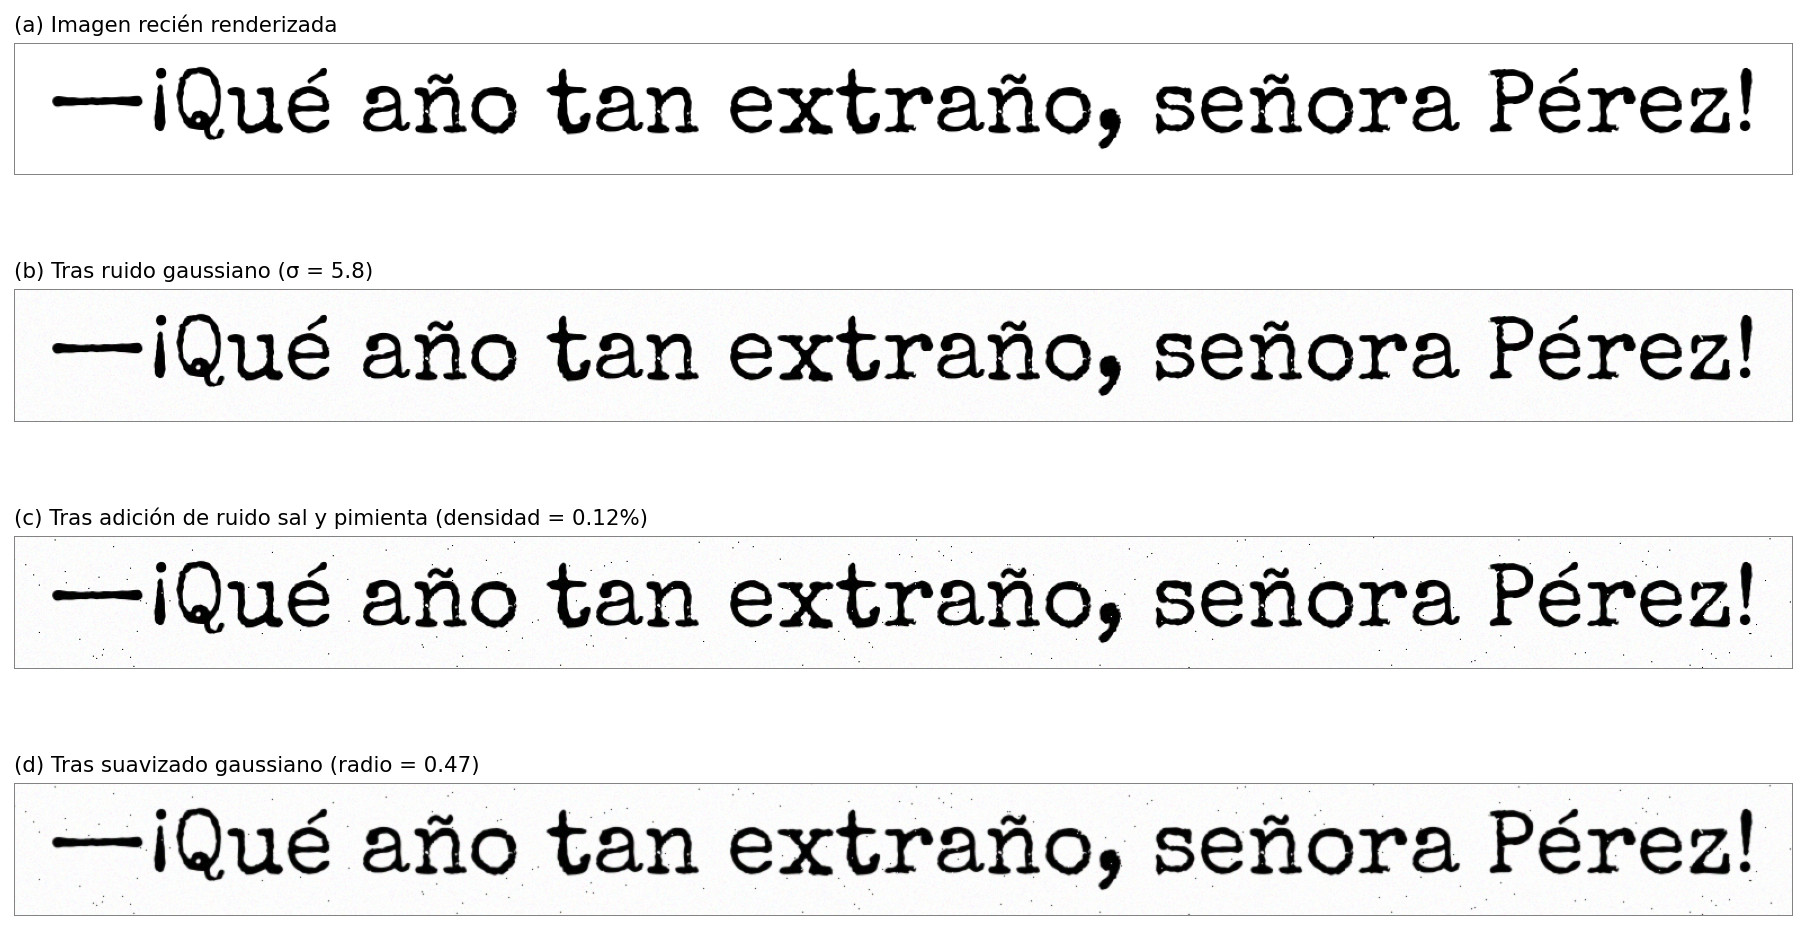
\includegraphics[width=\textwidth]{Graphics/degradacion_visual.png}
	\caption{Etapas acumulativas de la simulación de degradación visual sobre una línea recién renderizada del \textit{corpus} sintético, con la fuente SpecialElite. El panel~(a) muestra la imagen original tras el renderizado. El panel~(b) muestra la imagen tras la adición de ruido gaussiano con desviación típica~$\sigma$. El panel~(c) muestra la imagen tras la adición posterior de ruido sal y pimienta. El panel~(d) muestra la imagen tras el suavizado gaussiano final, que el sistema aplica al 50\,\% de las imágenes que escoge al azar. Los parámetros concretos que cada panel reporta corresponden a una realización aleatoria con los rangos que el texto describe.}
	\label{fig:degradacion-visual}
\end{figure}

La compatibilidad con ambos métodos de binarización es la propiedad que justifica la elección de las tres transformaciones y excluye otras alternativas. Otsu~\cite{otsu1979threshold} calcula un umbral global a partir del histograma bimodal de la imagen completa; Sauvola~\cite{sauvola2000binarization} calcula un umbral local para cada píxel a partir de la media y la desviación típica de los valores de gris en una vecindad. Las tres transformaciones modifican las estadísticas de niveles de gris de forma acotada y controlada, lo que permite a ambos métodos producir una binarización coherente sin perder caracteres. Transformaciones que alteren la geometría de los caracteres, como deformaciones elásticas o rotaciones agresivas, romperían la correspondencia entre la imagen y su transcripción y producirían etiquetas incorrectas. El capítulo~\ref{chap:preprocesamiento} ofrece la descripción de los dos métodos de binarización y del criterio de selección automática.

% -----------------------------------------------------------------------------
\section{Vocabulario indexado del sistema}
\label{sec:vocabulario}

El vocabulario de un sistema OCR es el conjunto cerrado de símbolos que el modelo puede producir como salida, cada uno asociado a un índice numérico. En cada paso temporal, la red CRNN produce un vector de probabilidades cuya dimensión coincide con el tamaño del vocabulario más uno. El paso adicional corresponde al \textit{token blank} propio de la función de pérdida CTC, que el capítulo~\ref{chap:modelo} describe.

El vocabulario del sistema comprende cien símbolos producibles, que el trabajo organiza de acuerdo con las convenciones de los marcos de entrenamiento OCR con CTC. La organización es la siguiente:

\begin{itemize}
	\item El índice cero corresponde al espacio en blanco, colocado en primera posición por ser el carácter más frecuente en cualquier texto corrido.
	\item Los índices uno a treinta y tres corresponden a las letras minúsculas del español, ordenadas por frecuencia objetivo descendente.
	\item Los índices treinta y cuatro a sesenta y seis corresponden a las letras mayúsculas en el mismo orden.
	\item Los índices sesenta y siete a setenta y seis corresponden a los dígitos del cero al nueve.
	\item Los índices setenta y siete a noventa y nueve corresponden a los signos de puntuación y a los símbolos tipográficos, ordenados también por frecuencia objetivo descendente.
	\item El índice cien queda reservado para el \textit{token blank} de CTC, que el marco de entrenamiento gestiona internamente sin que el modelo lo produzca como símbolo.
\end{itemize}

La organización por frecuencia objetivo descendente no es arbitraria. Algunos marcos de entrenamiento inicializan los sesgos de la capa de salida en función del índice, y mantener los símbolos más frecuentes con índices bajos puede acelerar la convergencia en las primeras épocas. La asignación explícita del índice cien al \textit{blank}, en lugar del índice cero como en algunos marcos, es una decisión consistente con el marco de entrenamiento que el sistema adopta. El capítulo~\ref{chap:modelo} ofrece la descripción del marco.

Al definir el vocabulario y generar el \textit{corpus}, el último paso del trabajo que el presente capítulo describe consiste en verificar las propiedades estadísticas del resultado.

% -----------------------------------------------------------------------------
\section{Análisis exploratorio del \textit{corpus} generado}
\label{sec:eda-corpus}

El análisis exploratorio del \textit{corpus} verifica que el resultado del procedimiento de generación satisface las propiedades de diseño que las secciones anteriores describen. El trabajo aplica el procedimiento a todo \textit{corpus} que el generador produce, antes de considerarlo apto para entrenamiento. La presente sección documenta el procedimiento y reporta los resultados sobre el \textit{corpus} de entrenamiento del sistema, que reúne 19\,998 imágenes que el generador produce con las nueve fuentes tipográficas que la subsección~\ref{subsec:fuentes-entrenamiento} describe. El procedimiento de análisis es idéntico para cualquier \textit{corpus} que el generador produzca, con independencia del repertorio tipográfico que emplee.

El análisis cubre cinco dimensiones: distribución de imágenes entre fuentes, longitudes de etiqueta, dimensiones de imagen, cobertura del vocabulario y frecuencias de caracteres. La figura~\ref{fig:eda-dashboard} reúne las visualizaciones del análisis en un único panel.

\begin{figure}[!htbp]
	\centering
	
\includegraphics[width=0.85\textwidth]{Graphics/eda_dashboard.png}
	\caption{Análisis exploratorio del \textit{corpus} sintético de entrenamiento, con 19\,998 imágenes que el generador produce a partir de las nueve fuentes tipográficas seleccionadas. El panel reúne las distribuciones de imágenes por fuente, longitudes de etiqueta, anchos, frecuencias de caracteres, cobertura del vocabulario español, cumplimiento de la restricción CTC, alturas por fuente y aspect ratio de las imágenes.}
	\label{fig:eda-dashboard}
\end{figure}

La distribución de imágenes entre fuentes resultó perfectamente uniforme, con 2\,222 imágenes por cada una de las nueve fuentes y un cociente entre la frecuencia máxima y la mínima igual a la unidad. La uniformidad garantiza que ninguna fuente tipográfica recibe más peso que las demás durante el entrenamiento.

Las longitudes de etiqueta presentaron una media de 38,5 caracteres, mediana de 37 caracteres y rango entre 9 y 74 caracteres, con desviación típica de 13,8 caracteres. Los percentiles 5, 25, 75 y 95 fueron 19, 28, 48 y 64 caracteres, respectivamente. La distribución resultó suave, sin acumulaciones en los extremos, gracias al sorteo aleatorio de la longitud máxima por cadena que la subsección~\ref{subsec:cadenas-balanceadas} describió.

Las dimensiones de imagen presentaron media de ancho de 1\,704 píxeles, mediana de 1\,630 píxeles, rango entre 229 y 3\,616 píxeles, y coeficiente de variación del 37,9\,\%. La altura la determinan el tamaño de fuente fijo y los márgenes, y presentó una media de 121 píxeles y rango entre 79 y 142 píxeles. La variabilidad del ancho es coherente con el rango de longitudes de etiqueta y con la diferencia de ancho entre fuentes monoespacio y fuentes serif para textos de la misma longitud. El análisis verificó el cumplimiento de la restricción que la función de pérdida CTC impone por inspección directa de cada par imagen--etiqueta: ninguna de las 19\,998 imágenes viola la restricción, según la cual el ancho de la imagen debe ser mayor o igual que la longitud de la etiqueta multiplicada por el factor de reducción horizontal de la red convolucional. El capítulo~\ref{chap:modelo} describe el detalle de la restricción.

La cobertura del vocabulario fue total: los cien símbolos del vocabulario del sistema están presentes en el \textit{corpus}, y ningún carácter del \textit{corpus} queda fuera del vocabulario. El \textit{corpus} reúne 770\,027 caracteres distribuidos en 147\,825 palabras, de las cuales 15\,001 son únicas. El coeficiente de variación de las frecuencias de caracteres alcanzó el 203,2\,\%, valor esperable en lenguaje natural dada la ley de Zipf~\cite{zipf1949human} que el capítulo~\ref{chap:estado-arte} introdujo.

Los caracteres específicos del español formal cubren todos el umbral mínimo de 500 apariciones. Las vocales con tilde (á, é, í, ó, ú) y la diéresis presentaron entre 1\,986 y 4\,705 apariciones cada una. La eñe alcanzó 3\,343 apariciones, las comillas angulares 3\,338 y 3\,335, y la raya de diálogo 6\,052. Los signos de apertura de interrogación y exclamación superaron 3\,300 apariciones cada uno. Tres símbolos genéricos quedaron por debajo del umbral: el corchete izquierdo (85 apariciones), el corchete derecho (83) y la almohadilla (87). Los tres son símbolos de uso poco frecuente en el español formal y no figuran entre los caracteres específicos del idioma. El procedimiento de generación los incluye en el vocabulario por exhaustividad, sin priorizar su sobremuestreo por encima de los caracteres del español. La métrica de cobertura mínima por carácter, que cubre los símbolos propios del idioma, resulta satisfactoria.

El análisis exploratorio confirma que el procedimiento de generación produce un \textit{corpus} conforme al diseño: balanceado entre fuentes, con longitudes de etiqueta en un rango operativo, con la representación total del vocabulario, con todos los caracteres específicos del español cubiertos por encima del umbral mínimo, y sin pares imagen--etiqueta que violen la restricción de la función de pérdida CTC.

% -----------------------------------------------------------------------------
% Transición al capítulo 3
% -----------------------------------------------------------------------------

Con el \textit{corpus} ya generado, validado y conforme al diseño, el capítulo cierra. El capítulo siguiente aborda la segunda contribución técnica del trabajo: el \textit{pipeline} de preprocesamiento que transforma documentos digitalizados reales en una secuencia de líneas de texto que sigue el formato que el modelo de reconocimiento espera.

	% Numeración del capítulo: 3.
\setcounter{chapter}{2}

\chapter{\textit{Pipeline} de preprocesamiento}\label{chap:preprocesamiento}

El presente capítulo describe el segundo componente técnico del sistema: el \textit{pipeline} de preprocesamiento que transforma una imagen de página digitalizada en una lista de líneas de texto listas para su procesamiento por el modelo de reconocimiento que el capítulo~\ref{chap:modelo} desarrolla. El capítulo se organiza en cinco secciones. La sección~\ref{sec:analisis-imagen} describe el análisis preliminar de la imagen y la configuración automática del \textit{pipeline} a partir de las métricas que el análisis produce. La sección~\ref{sec:binarizacion} detalla la binarización y el criterio de selección automática entre los dos métodos disponibles. La sección~\ref{sec:correccion-inclinacion} expone la corrección de inclinación a tres niveles: global de la página, residual por bloque y por línea. La sección~\ref{sec:deteccion-segmentacion} explica la detección de bloques de texto y la segmentación de líneas dentro de cada bloque. La sección~\ref{sec:normalizacion-lineas} describe la normalización final que produce las líneas con la altura fija que el modelo exige.

% -----------------------------------------------------------------------------
\section{Análisis de imagen y configuración automática}
\label{sec:analisis-imagen}

Las imágenes que el sistema recibe como entrada presentan una diversidad amplia de condiciones visuales. Una digitalización profesional de un libro tiene fondo claro y uniforme, iluminación homogénea, contraste alto y trazos nítidos. Una fotografía tomada con un teléfono móvil puede presentar gradientes de iluminación, sombras locales, ruido del sensor y baja resolución. Un documento antiguo digitalizado puede tener fondo amarillento, tinta desvanecida, manchas y desalineación. Cada condición exige parámetros distintos en las etapas posteriores del \textit{pipeline}.

Una primera opción consistiría en exponer los parámetros del \textit{pipeline} al usuario y dejar que los ajustara para cada imagen. El trabajo descarta la opción por dos razones. Primero, el usuario objetivo del sistema es un investigador o archivista que carece de formación en procesamiento de imágenes. Segundo, el ajuste manual para cada documento es incompatible con el procesamiento por lotes que requiere la digitalización masiva del acervo. El \textit{pipeline} adopta en su lugar una estrategia de configuración automática, que utiliza el cálculo de ciertas métricas de la imagen para definir los parámetros de la configuración.

El análisis calcula cinco métricas sobre la imagen en escala de grises. La primera es el contraste, que el sistema define como la diferencia entre los percentiles~95 y~5 de los valores de gris. La elección de percentiles, en lugar del rango máximo y mínimo, descarta píxeles anómalos que producen los reflejos puntuales o el ruido aislado. La segunda es la luminancia media. La tercera es la polaridad del fondo, que el sistema define a partir de la media de las esquinas de la imagen, con exclusión de franjas laterales que podrían contener bandas oscuras de encuadernación. Si la media de las esquinas resulta inferior a~127, el sistema considera oscuro el fondo y la binarización posterior invierte. La cuarta y la quinta son la altura estimada del texto y el número estimado de líneas, que el análisis calcula a partir de la proyección horizontal de una binarización preliminar mediante Otsu~\cite{otsu1979threshold}, con identificación de picos por la función \textit{find\_peaks} sobre la proyección que un filtro uniforme suaviza. La figura~\ref{fig:metricas-ejemplo} ilustra los valores que el análisis produce sobre una página real del archivo, junto con las decisiones de configuración que las cinco métricas inducen.

\begin{figure}[!htbp]
	\centering
	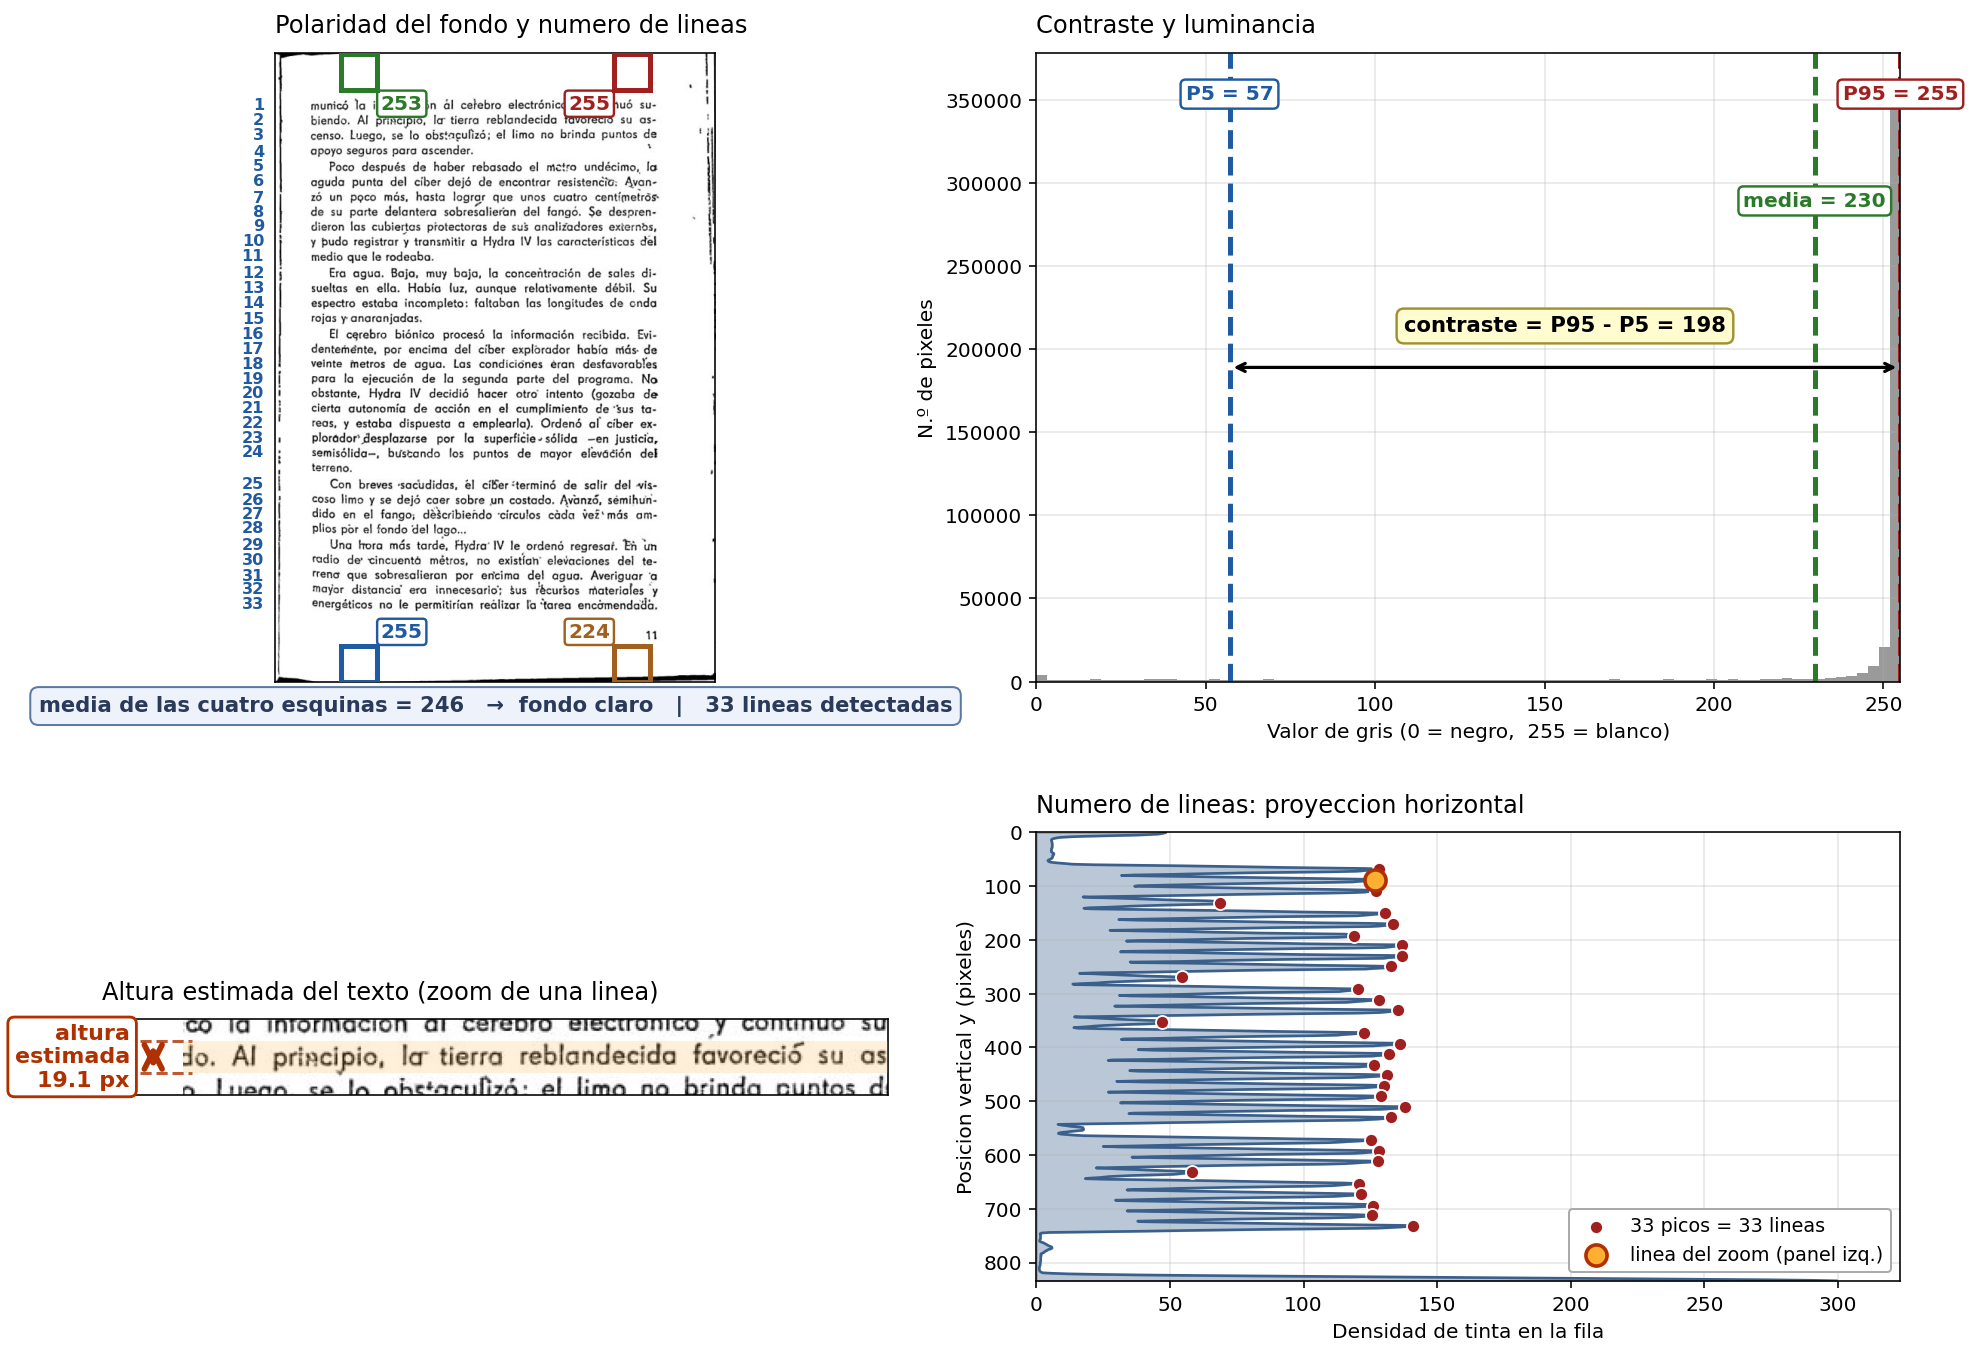
\includegraphics[width=\textwidth]{Graphics/analisis_metricas.png}
	\caption{Visualización de las cinco métricas que el análisis preliminar produce sobre una página real del archivo. El panel superior izquierdo muestra la imagen original con las cuatro esquinas que el sistema muestrea para decidir la polaridad del fondo y con la numeración de las líneas detectadas. El panel superior derecho muestra el histograma de intensidades con los percentiles~5 y~95, la luminancia media y el contraste como diferencia entre ambos percentiles. El panel inferior izquierdo presenta el zoom de una línea concreta con la cota de la altura estimada del texto. El panel inferior derecho muestra la proyección horizontal de la tinta, con cada pico que corresponde a una línea; el pico naranja resalta la línea que el panel del zoom amplía.}
	\label{fig:metricas-ejemplo}
\end{figure}

Las cinco métricas alimentan una función de configuración automática que devuelve los parámetros del \textit{pipeline}. Las decisiones de la configuración son las siguientes:

\begin{enumerate}[leftmargin=*,labelsep=0.5em]
	\item \textbf{Ecualización adaptativa del histograma.} Si el contraste cae por debajo de~60, el sistema activa la ecualización adaptativa del histograma con limitación de contraste, que la literatura denomina CLAHE~\cite{zuiderveld1994clahe} por sus siglas inglesas, junto con un filtro bilateral que reduce el ruido sin difuminar los bordes.
	\item \textbf{Ventana de Sauvola.} El sistema dimensiona la ventana del método de Sauvola~\cite{sauvola2000binarization} en función de la altura estimada del texto, garantizando que la vecindad de análisis cubra al menos una vez y media la altura de un carácter.
	\item \textbf{Parámetro $k$ de Sauvola.} El sistema ajusta el parámetro de sensibilidad de Sauvola en tres tramos según el contraste, con valores entre~0,10 y~0,25.
	\item \textbf{Inversión binaria.} El sistema activa la inversión cuando el fondo resulta oscuro, según la polaridad que la tercera métrica determina.
	\item \textbf{Dilatación vertical y altura mínima por línea.} El sistema calibra la dilatación vertical que la detección de líneas emplea, y la altura mínima que admite por línea, sobre la altura estimada del texto.
\end{enumerate}

El resultado del análisis es una configuración del \textit{pipeline} adaptable a las particularidades de cada imagen sin intervención del usuario. El \textit{pipeline} aplica la configuración en las etapas siguientes, que la presente sección describe a continuación.

% -----------------------------------------------------------------------------
\section{Binarización}
\label{sec:binarizacion}

La binarización es la operación que asigna a cada píxel el valor 0 si pertenece al fondo o el valor 1 si pertenece a tinta. La operación es necesaria por dos razones. La primera es que las etapas posteriores del \textit{pipeline}, como la detección de bloques y la segmentación de líneas, operan sobre proyecciones y componentes conexas existentes solo en imágenes binarias. La segunda es que la binarización elimina la variabilidad cromática y tonal de la imagen original, reduciendo el espacio de variación que el modelo debe aprender a tolerar.

El \textit{pipeline} dispone de dos métodos de binarización con propiedades complementarias. El primer método es la binarización global de Otsu~\cite{otsu1979threshold}, que calcula un único umbral para toda la imagen a partir del histograma bimodal de los valores de gris. El método escoge el umbral como el valor que maximiza la varianza entre las dos clases, una correspondiente al fondo y la otra a la tinta. Otsu produce trazos con el grosor natural del raster original, lo que resulta deseable cuando el fondo es uniforme y la separación entre tinta y papel es clara. El segundo método es la binarización adaptativa de Sauvola~\cite{sauvola2000binarization}, que calcula un umbral local para cada píxel a partir de la media~$\mu$ y la desviación típica~$\sigma$ de los valores de gris en una vecindad de tamaño fijo. El umbral local resulta de la fórmula:

\begin{equation}
	T(x, y) = \mu(x, y)\left[1 + k \left(\frac{\sigma(x, y)}{R} - 1\right)\right],
	\label{eq:sauvola}
\end{equation}

donde $k$ es un parámetro de sensibilidad y~$R$ es el rango dinámico esperado de la desviación típica. Sauvola compensa variaciones de iluminación que un umbral global no podría capturar, a costa de engrosar los trazos en aproximadamente el 15--25\,\% respecto al grosor natural.

La selección automática del método se basa en una medida de uniformidad del fondo. El \textit{pipeline} estima la desviación típica de los píxeles de fondo de la imagen tras una binarización preliminar y compara el valor con un umbral empírico que el sistema fija en~12. Por debajo del umbral, el sistema considera uniforme el fondo y aplica Otsu. Por encima, aplica Sauvola. El trabajo calibró el umbral sobre un conjunto pequeño de imágenes de prueba que abarcan tanto digitalizaciones limpias de libros como fotografías con iluminación irregular.

Tras la binarización, el \textit{pipeline} aplica una secuencia de operaciones de limpieza. La apertura morfológica~\cite{soille2003morphology} con un elemento estructurante cuadrado de dos píxeles elimina el moteado fino. El filtrado de componentes conexos descarta cualquier componente con área inferior a cuatro píxeles, valor por debajo del tamaño de los puntos sobre las íes y de los acentos en cualquier tipografía razonable, sin afectar al texto legítimo. La salida es una imagen binaria limpia, lista para las etapas siguientes.

% -----------------------------------------------------------------------------
\section{Corrección de inclinación y curvatura}
\label{sec:correccion-inclinacion}

Las imágenes de documentos digitalizados rara vez presentan las líneas de texto perfectamente horizontales. Una digitalización hecha a mano puede introducir una rotación leve de hasta tres o cuatro grados. Una fotografía de un teléfono móvil añade además distorsión perspectiva que curva el \textit{baseline} de las líneas. Un libro entero digitalizado presenta inclinaciones distintas en cada página del pliego, y a veces incluso en cada columna. El \textit{pipeline} corrige la inclinación a tres niveles sucesivos, cada uno con un alcance espacial diferente.

El primer nivel es la corrección global de la página. La operación, que la literatura denomina \textit{deskew}, busca el ángulo de rotación que devuelve las líneas de texto a la horizontalidad sobre la imagen completa. El método descansa sobre la transformada de Hough~\cite{duda1972hough}, en su variante probabilística. Hough no opera directamente sobre la imagen binaria, donde cada glifo es un cúmulo denso de píxeles que generaría falsas líneas, sino sobre una imagen de bordes que el operador de Canny~\cite{canny1986edge} produce en un paso previo. Canny suaviza la imagen con un filtro gaussiano, calcula los gradientes mediante un operador tipo Sobel, suprime los píxeles que no son máximos locales del gradiente y aplica una umbralización por histéresis con dos umbrales, en este caso~50 y~150. El resultado es una imagen donde solo los píxeles de contorno están activos, lo que reduce cada glifo a su silueta y deja una nube de puntos que cae aproximadamente sobre los \textit{baselines} de cada línea. Hough sobre esos contornos identifica segmentos rectos, cada uno con un ángulo, que el sistema pondera por el cuadrado de su longitud. La ponderación cuadrática hace que los segmentos largos, que corresponden a los \textit{baselines} de líneas completas, dominen sobre los segmentos cortos que generan los trazos oblicuos de letras individuales. El ángulo de corrección es la mediana ponderada de la distribución, que el sistema descarta cuando el rango intercuartílico supera cuatro grados, lo que indicaría una distribución multimodal incompatible con una única inclinación global.

El segundo nivel es la corrección residual por bloque, que el \textit{pipeline} aplica después de la corrección global. La operación ataca el caso de páginas con dos columnas o pliegos abiertos donde cada bloque presenta su propia inclinación residual respecto a la página. La estimación del ángulo opera con un método análogo al del nivel global, que el sistema restringe al recorte del bloque y con un rango angular más conservador.

El tercer nivel es la corrección de curvatura por línea, que la literatura denomina \textit{straightening}~\cite{zhang2002straightening}. La operación corrige las distorsiones que sobreviven a las correcciones lineales anteriores, típicamente el sangrado central que aparece en la digitalización de páginas cerca del lomo del libro y la curvatura que generan las fotografías con perspectiva. El método estima el \textit{baseline} de la línea como una curva polinomial de grado dos. Para construir la estimación, el método divide la línea en rebanadas verticales y calcula el centroide vertical de la tinta dentro de cada rebanada. Un ajuste por mínimos cuadrados aproxima el conjunto de pares (centro horizontal de la rebanada, centroide vertical de la tinta) a un polinomio de grado dos. El método acepta el ajuste solo si el coeficiente de determinación supera~0,72 y si el desplazamiento implícito no excede el 20\,\% de la altura de la línea. La aceptación condicional protege contra correcciones espurias en líneas demasiado cortas o con tinta dispersa, donde el ajuste polinomial podría sobreajustarse al ruido.

El conjunto de las tres correcciones cubre el rango de distorsiones que el sistema puede encontrar en la práctica, desde la rotación global uniforme hasta la curvatura local del \textit{baseline}.

% -----------------------------------------------------------------------------
\section{Detección y segmentación de bloques y líneas de texto}
\label{sec:deteccion-segmentacion}

El modelo de reconocimiento opera sobre líneas de texto individuales. El \textit{pipeline} debe, por tanto, identificar dónde empieza y termina cada línea dentro de la imagen binarizada. La identificación procede en dos fases. La primera identifica bloques de texto sobre la página completa. La segunda segmenta líneas dentro de cada bloque.

\subsection{Detección de bloques de texto}

Una página puede contener un único bloque de texto continuo, varias columnas paralelas, o un pliego con dos páginas separadas por un margen central. La detección de bloques separa la estructura espacial de la página antes de procesar las líneas. El método descansa sobre una variante recursiva del algoritmo XY-Cut, que alterna cortes horizontales y verticales sobre la imagen binarizada para descomponer la página en regiones rectangulares.

El algoritmo aplica tres niveles sucesivos. El primer nivel busca separadores horizontales globales sobre toda la imagen mediante la proyección horizontal de la tinta. Las franjas con densidad inferior al~4\,\% del máximo y altura superior a un umbral mínimo actúan como separación entre secciones, y dividen la página en bandas horizontales. El segundo nivel busca, dentro de cada banda, separadores verticales que detecten columnas paralelas. La búsqueda procede por análisis de picos sobre la proyección vertical: cada par de picos consecutivos define una columna candidata, con el valle entre ambos como posible separador. El tercer nivel aplica de nuevo la búsqueda de separadores horizontales dentro de cada columna, lo que permite separar bloques internos como cabeceras, párrafos aislados o pies de página dentro de la misma columna.

La búsqueda del valle entre dos columnas no opera por simple mínimo de la proyección. El método que el \textit{pipeline} aplica es una detección bilateral del hueco: desde cada uno de los dos picos el algoritmo camina hacia el otro hasta que la densidad de tinta cae por debajo de un umbral situado a media profundidad del valle. Los dos puntos de cruce delimitan el ancho real del hueco entre columnas, y el método coloca el separador en el centro de ese intervalo. La técnica protege contra una distorsión que aparece con frecuencia en libros encuadernados: el moteado central del lomo introduce una densidad residual que no rompe la condición de valle pero desplaza el mínimo absoluto hacia uno de los lados, dejando el separador pegado al borde del texto de una de las dos páginas. La figura~\ref{fig:xy-cut} ilustra el procedimiento sobre un pliego digitalizado del archivo: la proyección vertical revela los picos que corresponden a cada columna, y el método coloca el separador en el centro del valle que separa las dos páginas.

\begin{figure}[!htbp]
	\centering
	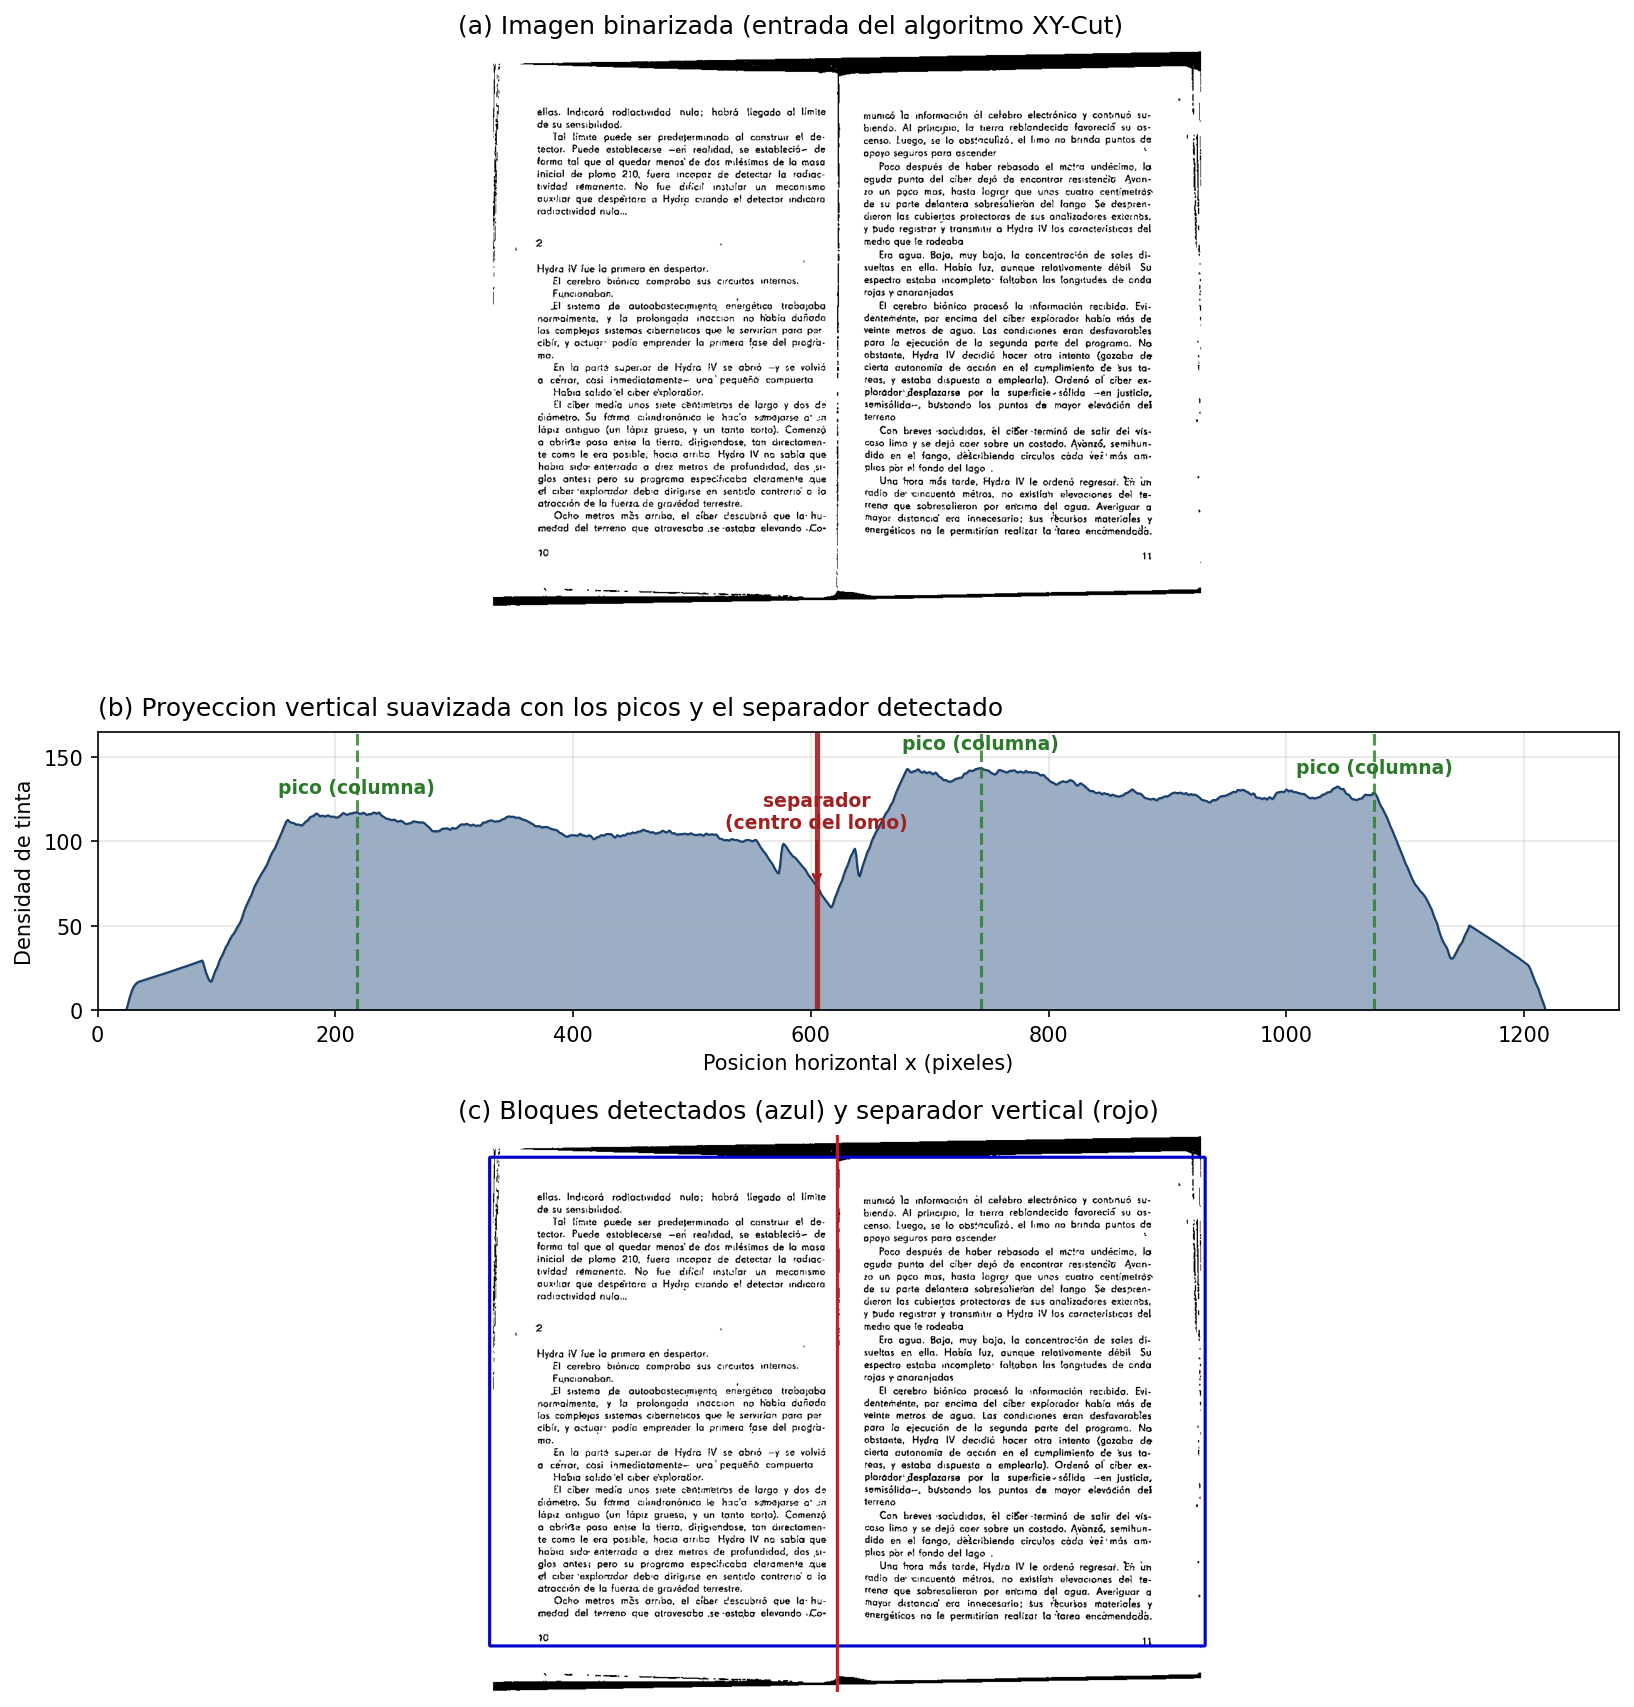
\includegraphics[width=0.95\textwidth]{Graphics/xy_cut_proceso.png}
	\caption{Detección de bloques sobre un pliego digitalizado mediante el algoritmo XY-Cut. El panel (a) muestra la imagen binarizada que sirve de entrada al algoritmo. El panel (b) muestra la proyección vertical tras el suavizado, los picos que corresponden a cada columna y el separador que el método coloca en el centro del hueco entre páginas. El panel (c) muestra los bloques detectados sobre la imagen original.}
	\label{fig:xy-cut}
\end{figure}

El candidato a separador se acepta solo si la profundidad del valle supera el 28\,\% de la altura del pico menor de los dos, si el ancho del hueco supera un umbral mínimo, y si la posición del separador queda dentro del rango central del 15 al 85\,\% del ancho de la imagen. La triple condición rechaza separadores que aparecerían en imágenes con una sola columna pero con variaciones locales de densidad. El algoritmo admite hasta cuatro columnas por banda; cuando el número de candidatos excede el límite, el sistema conserva los separadores con la profundidad de valle mayor.

Antes de aplicar el algoritmo, una máscara cubre las franjas laterales que corresponden a la encuadernación. La medida evita que el moteado oscuro del borde del escáner aparezca como contenido de texto y desplace los cortes hacia el interior de la página. Tras la segmentación, el sistema fusiona en un único bloque los bloques resultantes que quedan a una distancia inferior a un umbral, lo que evita la sobresegmentación de columnas que el algoritmo dividió en exceso por la presencia de espacios verticales puntuales dentro del texto.

\subsection{Segmentación de líneas dentro de cada bloque}

Dentro de cada bloque, el \textit{pipeline} segmenta las líneas mediante proyección horizontal con dilatación morfológica previa. La dilatación horizontal une las palabras de una misma línea para que la proyección presente un máximo continuo a lo largo del renglón. La dilatación vertical, mucho más pequeña, conecta los acentos de las mayúsculas con el cuerpo de la letra correspondiente, lo que evita que los acentos generen picos secundarios en la proyección.

Un filtro uniforme suaviza la proyección horizontal resultante. El método umbraliza la proyección suavizada con un valor que el método de Otsu~\cite{otsu1979threshold} produce sobre el perfil unidimensional. El umbral final queda acotado al~25\,\% del pico máximo de la proyección, valor que el trabajo calibró para que las líneas cortas de final de párrafo, cuya proyección puede ser entre tres y cinco veces menor que la de líneas completas, queden por encima del umbral.

La salida de la segmentación es una lista de cajas delimitadoras, con las coordenadas verticales y horizontales de cada esquina del segmento en la imagen original. El algoritmo expande ligeramente cada caja hacia los píxeles de tinta adyacentes que probablemente quedaran fuera del corte estricto por proyección. La línea final corresponde al recorte de la imagen original en la región que delimita la caja expandida.

% -----------------------------------------------------------------------------
\section{Normalización de líneas para inferencia}
\label{sec:normalizacion-lineas}

Las líneas que salen del paso de segmentación presentan dimensiones heterogéneas. La altura varía con el tamaño tipográfico, la presencia de descendentes y ascendentes y el ajuste de la caja delimitadora. El ancho varía con la longitud del texto. El modelo de reconocimiento exige, sin embargo, una altura fija para sus entradas, según argumenta el capítulo~\ref{chap:modelo}. La sección describe el procedimiento de normalización que produce las líneas con el formato que el modelo espera.

El procedimiento se descompone en tres operaciones secuenciales. La primera es el recorte vertical. El sistema localiza las filas con presencia de tinta y recorta la línea a la región vertical mínima que las contiene, con un margen de seguridad dinámico igual al 10\,\% de la altura del texto. El margen evita que descendentes y ascendentes queden cortados por un ajuste demasiado ceñido.

La segunda operación es el redimensionado a una altura fija de~64 píxeles, manteniendo la proporción original entre alto y ancho. El trabajo eligió la altura fija de~64 píxeles por dos razones. La primera es la compatibilidad con la arquitectura convolucional del modelo: el codificador aplica cuatro reducciones de la altura por un factor de dos, lo que requiere que la altura de entrada sea divisible por~16. La segunda es el equilibrio entre detalle visual preservado y coste computacional. Alturas menores comprimen los caracteres hasta perder rasgos finos. Alturas mayores aumentan el coste de cómputo sin mejora apreciable en exactitud para los cuerpos tipográficos habituales en documentos impresos. El ancho resultante es variable y queda determinado por la proporción de la línea original.

La tercera operación es la conversión de la imagen a tensor en coma flotante con valores normalizados al intervalo $[0, 1]$. La operación produce el formato exacto que el modelo CRNN+CTC~\cite{shi2016crnn,graves2006ctc} consume como entrada durante la inferencia.

La contribución cuantitativa de cada etapa del \textit{pipeline} sobre el rendimiento del modelo final no se evalúa mediante un estudio de ablación específico en este trabajo. La razón es metodológica: cada etapa cumple una función no opcional dentro del flujo --la binarización produce la representación que el extractor convolucional del modelo espera, la corrección de inclinación habilita la proyección horizontal que la segmentación de líneas necesita, la segmentación produce las líneas que el modelo procesa, y la normalización ajusta la altura que la arquitectura impone--, por lo que su eliminación produciría una caída catastrófica de la métrica que un estudio de ablación constataría sin aportar información cuantitativa interpretable. La validación de cada técnica descansa, por tanto, en la evidencia empírica que la literatura previa aporta sobre documentos impresos: Otsu~\cite{otsu1979threshold} y Sauvola~\cite{sauvola2000binarization} sustentan la binarización adaptativa con selección entre umbral global y umbral local según el criterio de uniformidad de fondo, y Duda y Hart~\cite{duda1972hough} sustentan la transformada que detecta la orientación dominante para la corrección de inclinación. Un estudio de ablación que cuantifique la contribución marginal de cada parámetro de cada etapa sobre el \textit{corpus} propio constituye una línea natural de extensión del trabajo.

% -----------------------------------------------------------------------------
% Transición al capítulo 4
% -----------------------------------------------------------------------------

Con el \textit{pipeline} de preprocesamiento que el capítulo describe, queda cerrado el camino que transforma una página digitalizada en una lista de líneas con el formato que el modelo de reconocimiento espera. El capítulo siguiente aborda la tercera contribución técnica del trabajo: el diseño, el entrenamiento y la evaluación del modelo CRNN+CTC que produce la transcripción de cada línea normalizada.

	% Numeración del capítulo: 4.
\setcounter{chapter}{3}

\chapter{Diseño, entrenamiento y evaluación del modelo de reconocimiento}\label{chap:modelo}

El capítulo describe el componente central del sistema: el modelo que toma una línea de texto que el \textit{pipeline} de preprocesamiento del capítulo~\ref{chap:preprocesamiento} normaliza y produce su transcripción. El capítulo comprende siete secciones. La sección~\ref{sec:arquitectura} expone la arquitectura CRNN+CTC~\cite{shi2016crnn,graves2006ctc} y las propiedades que la justifican como elección. La sección~\ref{sec:implementacion-modelo} detalla los parámetros concretos de la implementación. La sección~\ref{sec:protocolo-entrenamiento} describe el protocolo de entrenamiento, con hiperparámetros, agrupación por anchos y augmentación de datos. La sección~\ref{sec:decodificacion} compara las dos estrategias de decodificación disponibles durante la inferencia y motiva la elección final. La sección~\ref{sec:evaluacion-estadistica} describe el protocolo de evaluación estadística que sustenta los resultados. La sección~\ref{sec:resultados-entrenamiento} reporta los resultados experimentales del entrenamiento principal. La sección~\ref{sec:fine-tuning} describe la etapa posterior de adaptación mediante \textit{fine-tuning} sobre un \textit{corpus} ampliado de fuentes tipográficas.

% -----------------------------------------------------------------------------
\section{Arquitectura CRNN+CTC}
\label{sec:arquitectura}

La arquitectura combina tres bloques funcionales que operan en cascada: un extractor de características visuales construido sobre una red neuronal convolucional, un codificador secuencial construido sobre una red neuronal recurrente bidireccional, y un cabezal de clasificación denso que la función de pérdida \textit{Connectionist Temporal Classification}~\cite{graves2006ctc} entrena. Shi, Bai y Yao~\cite{shi2016crnn} introdujeron el esquema general bajo el nombre CRNN, que entrena de extremo a extremo sobre pares imagen--transcripción sin necesidad de segmentar caracteres individualmente. La figura~\ref{fig:crnn-arquitectura} resume el flujo de datos completo, incluyendo la forma del tensor a la salida de cada capa para una imagen de altura sesenta y cuatro píxeles y ancho arbitrario~$W$.

\begin{figure}[!htbp]
	\centering
	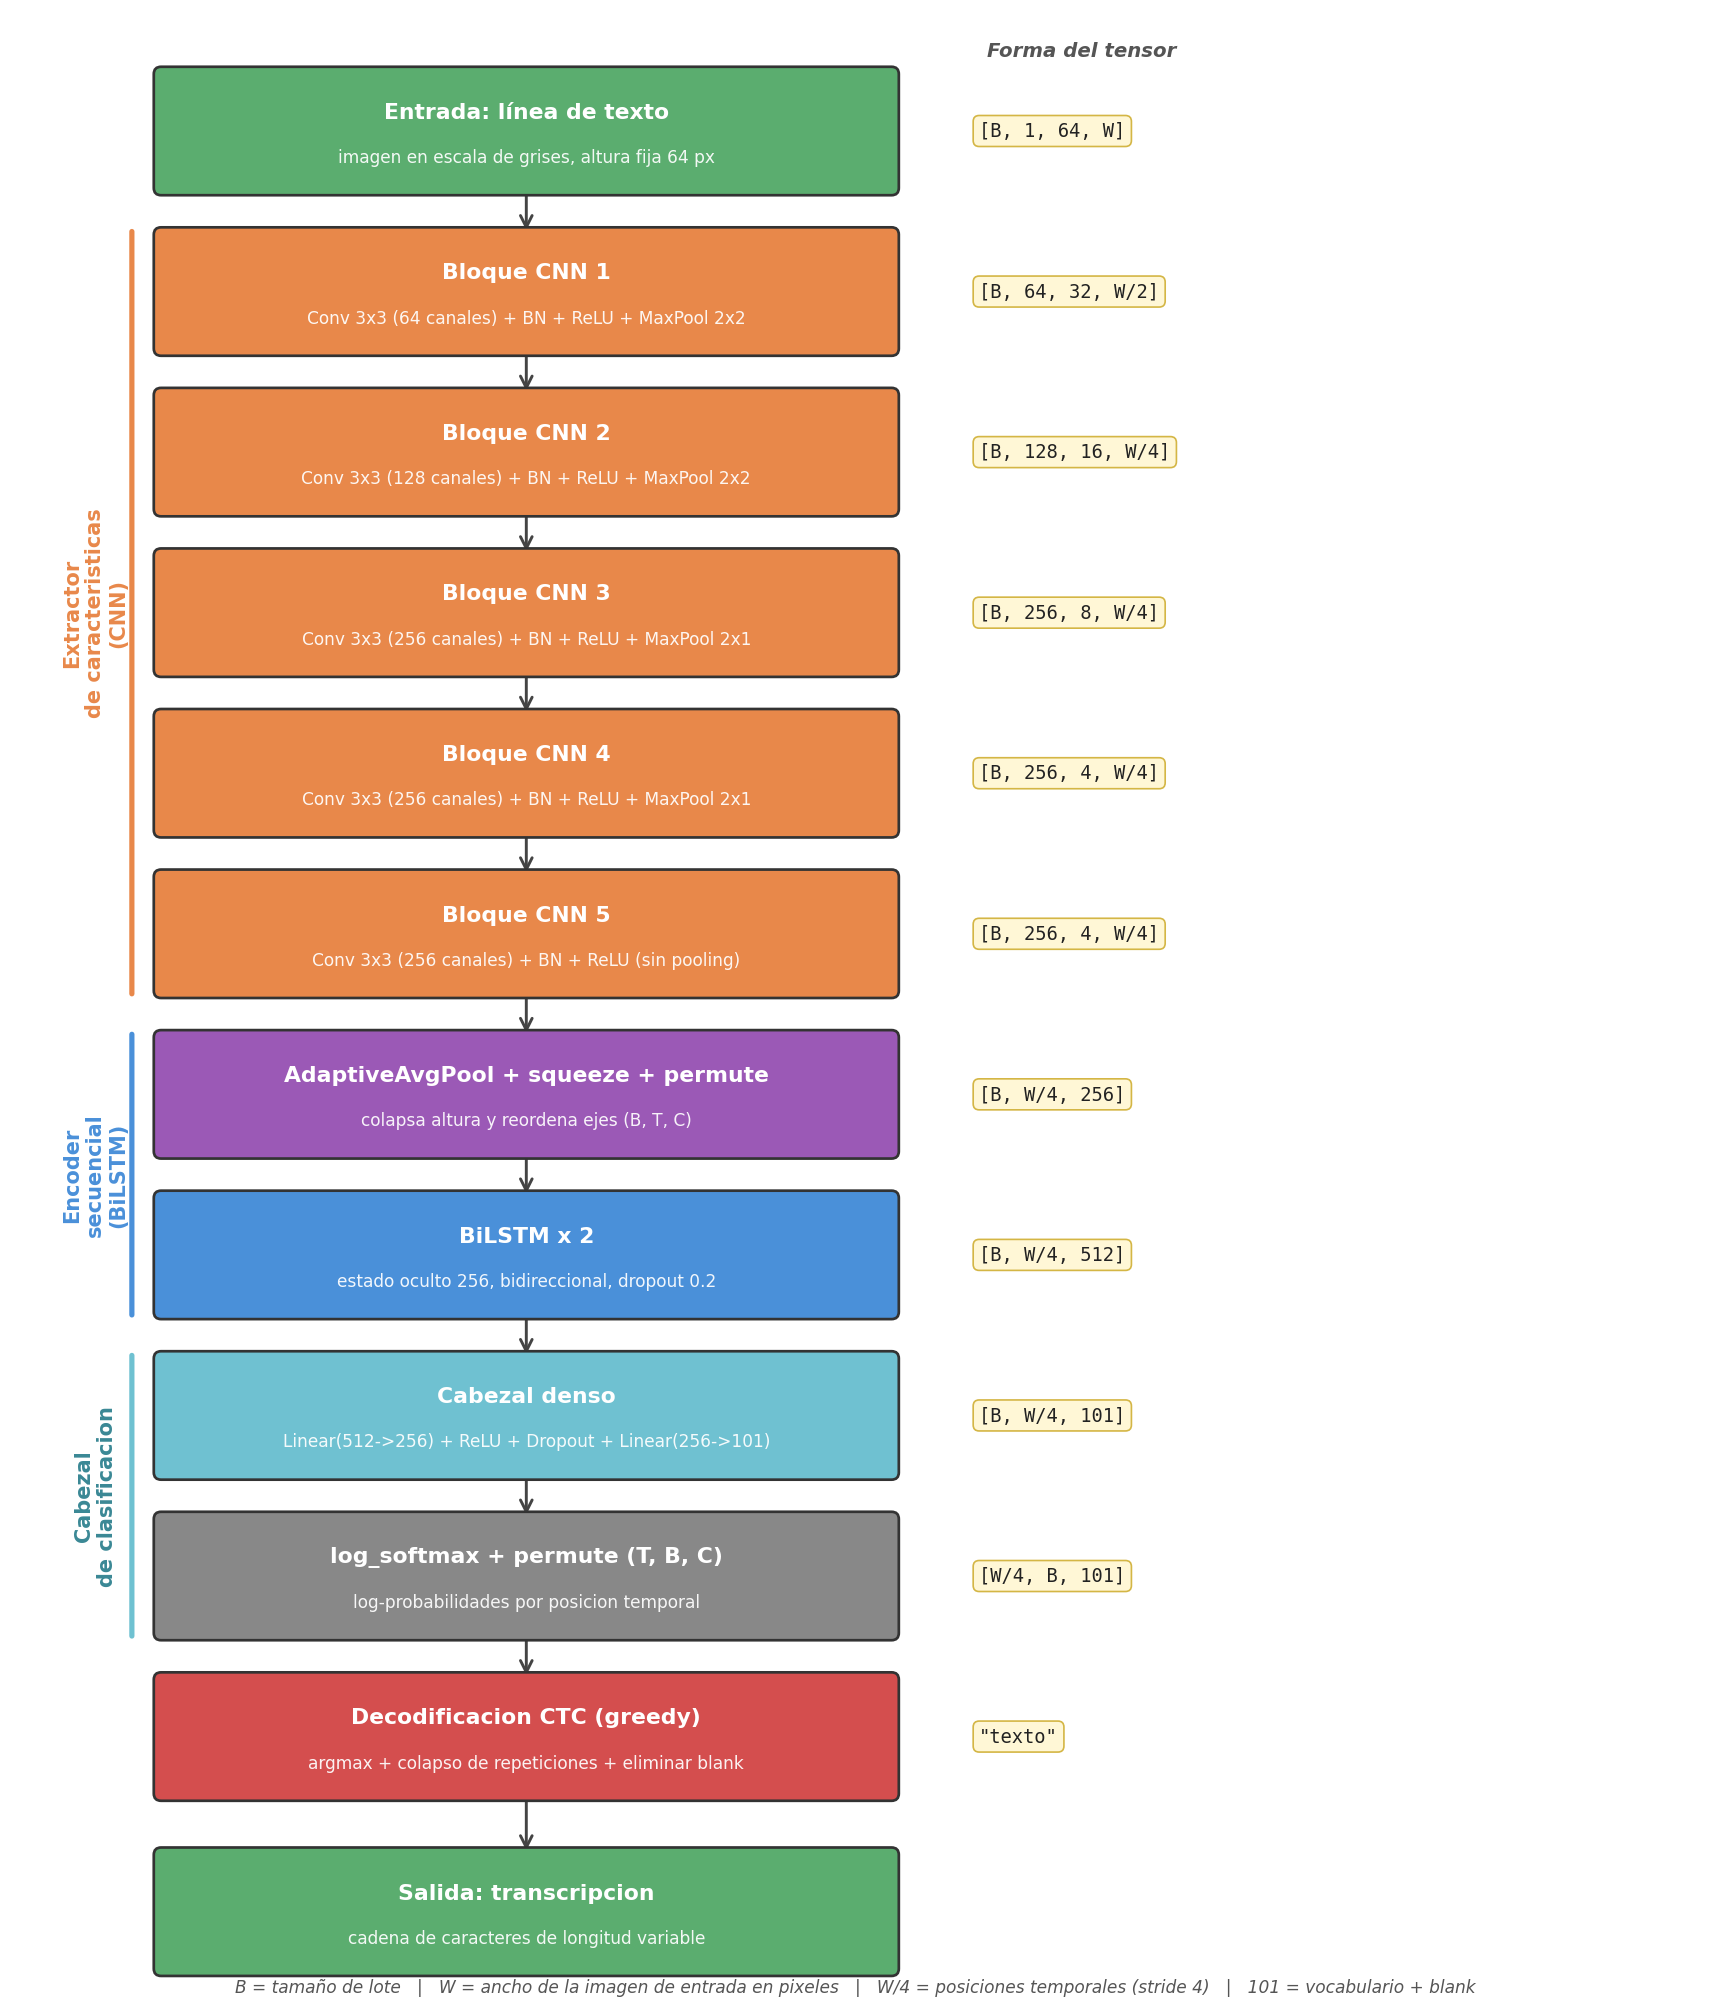
\includegraphics[width=0.92\textwidth]{Graphics/crnn_arquitectura.png}
	\caption{Diagrama del modelo CRNN+CTC para reconocimiento de líneas impresas. Cada caja representa una capa del modelo y la etiqueta amarilla a la derecha indica la forma del tensor a su salida. Las tres etiquetas verticales identifican los tres bloques funcionales: el extractor convolucional (cinco bloques CNN), el codificador secuencial (dos capas BiLSTM apiladas) y el cabezal de clasificación (capas densas seguidas de \textit{log-softmax} y decodificación CTC). El factor de reducción horizontal acumulado de la CNN es cuatro, por lo que el número de posiciones temporales que el modelo produce es la cuarta parte del ancho de la imagen de entrada en píxeles.}
	\label{fig:crnn-arquitectura}
\end{figure}

Las cuatro subsecciones siguientes describen brevemente los componentes y la restricción de longitud que la combinación impone sobre las entradas admisibles.

\subsection{Extractor convolucional}
\label{subsec:cnn-extractor}

El extractor procesa la imagen de la línea y produce una secuencia de vectores de características. Se compone de cinco bloques con \textit{kernel} cuadrado de tres por tres y \textit{padding} unitario, cada uno seguido de normalización por lotes y activación ReLU. Cuatro de los bloques incluyen una operación de \textit{max-pooling}: los dos primeros emplean una ventana cuadrada de dos por dos que reduce ambos ejes a la mitad, y los dos siguientes una ventana asimétrica de dos por uno que reduce solo la altura y preserva la resolución horizontal. La asimetría de los dos últimos \textit{pooling} es el rasgo que permite mantener una secuencia horizontal con resolución suficiente para alimentar al codificador recurrente. La tabla~\ref{tab:bloques-cnn} resume la configuración de los cinco bloques y la forma del tensor a la salida de cada uno.

\begin{table}[!htbp]
	\centering
	\caption{Configuración de los cinco bloques convolucionales del extractor. La columna \emph{Pooling} indica la reducción $(H \times W)$ que la operación aplica.}
	\label{tab:bloques-cnn}
	\footnotesize
	\begin{tabular}{ccccc}
		\toprule
		\textbf{Bloque} & \textbf{Convolución} & \textbf{Pooling} & \textbf{Reducción acumulada} & \textbf{Salida $(C, H, W)$} \\
		\midrule
		1 & Conv $3\times3$, 64 ch  & MaxPool $2\times2$ & $H/2,\ W/2$ & $(64,\ 32,\ W/2)$ \\
		2 & Conv $3\times3$, 128 ch & MaxPool $2\times2$ & $H/4,\ W/4$ & $(128,\ 16,\ W/4)$ \\
		3 & Conv $3\times3$, 256 ch & MaxPool $2\times1$ & $H/8,\ W/4$ & $(256,\ 8,\ W/4)$ \\
		4 & Conv $3\times3$, 256 ch & MaxPool $2\times1$ & $H/16,\ W/4$ & $(256,\ 4,\ W/4)$ \\
		5 & Conv $3\times3$, 256 ch & ---                & $H/16,\ W/4$ & $(256,\ 4,\ W/4)$ \\
		\bottomrule
	\end{tabular}
\end{table}

Una capa de \textit{adaptive-average-pooling} colapsa el eje de altura a uno, una operación de \textit{squeeze} elimina la dimensión unitaria, y una permutación de ejes reordena el resultado como una secuencia indexada por posiciones a lo largo del eje horizontal, con doscientos cincuenta y seis canales por posición. Cada vector codifica las características visuales de una franja vertical de la línea original con un ancho efectivo de cuatro píxeles.

\subsection{Codificador recurrente bidireccional}
\label{subsec:rnn-secuencial}

La secuencia que produce el extractor carece de modelado del contexto entre posiciones vecinas. Una franja vertical aislada es ambigua sin información del contexto adyacente: la franja central de una letra como ``l'' es visualmente indistinguible de la franja central de una letra como ``i'' o ``j'' sin información sobre el resto del trazo. El codificador recurrente aporta el contexto que se necesita para resolver las ambigüedades.

Se emplean dos capas apiladas del tipo \textit{Long Short-Term Memory}~\cite{hochreiter1997lstm}, conocido como LSTM por sus siglas en inglés, en modo bidireccional. La bidireccionalidad consiste en aplicar dos LSTM sobre la misma secuencia, una en sentido directo y otra en sentido inverso, y concatenar las salidas, de modo que cada posición de la secuencia codifica contexto tanto del prefijo como del sufijo. El estado oculto tiene dimensión doscientos cincuenta y seis por dirección, por lo que la salida concatenada en cada posición temporal es un vector de quinientas doce dimensiones.

\subsection{Función de pérdida CTC y \textit{token blank}}
\label{subsec:ctc-loss}

La salida del modelo es una secuencia de distribuciones de probabilidad sobre el vocabulario, indexada por posiciones temporales. La transcripción de referencia es una secuencia de símbolos, indexada por posiciones de la cadena. Las dos secuencias tienen, en general, longitudes distintas y no existe alineamiento explícito entre las posiciones de la primera y las de la segunda. La función de pérdida \textit{Connectionist Temporal Classification}, que el trabajo de Graves et~al.~\cite{graves2006ctc} introdujo originalmente, resuelve el problema sin alineación previa.

La idea central de CTC es introducir un símbolo adicional que la literatura denomina \textit{token blank}, que el modelo puede emitir en cualquier posición temporal sin que aparezca en la transcripción. CTC define la probabilidad de una transcripción como la suma sobre todos los alineamientos posibles entre las posiciones temporales y los símbolos de la transcripción, donde un alineamiento es válido si, tras eliminar las apariciones del \textit{token blank} y colapsar las repeticiones consecutivas del mismo símbolo, produce la transcripción de referencia. El número de alineamientos válidos crece de forma exponencial con la longitud de la secuencia y de la transcripción, por lo que su enumeración explícita es inviable. La pérdida CTC es el logaritmo negativo de la probabilidad agregada de la transcripción, y el algoritmo de \textit{forward-backward}~\cite{graves2006ctc} la calcula en tiempo polinomial mediante programación dinámica, de forma análoga al algoritmo que opera sobre los modelos ocultos de Markov. El algoritmo recorre las posiciones temporales y acumula, para cada par formado por una posición temporal y una posición en la transcripción que intercala \textit{blanks}, la probabilidad agregada de los caminos parciales que llegan a ese estado, lo que permite obtener la probabilidad total sin enumerar caminos individuales.

El \textit{token blank} cumple dos funciones complementarias. La primera es absorber posiciones temporales donde el modelo aún no se compromete con la emisión de un símbolo concreto, condición que se manifiesta como tramos de baja confianza en la salida. La segunda es separar repeticiones legítimas del mismo símbolo: sin \textit{token blank}, una transcripción como ``mejilla'' produciría una sola ``l'' tras el colapso de repeticiones; la presencia del \textit{token blank} entre las dos eles permite preservar la repetición. El vocabulario del sistema contiene los cien símbolos producibles que el capítulo~\ref{chap:corpus} describe, más el \textit{token blank}, que el sistema asigna por convención al índice cien.

\subsection{\textit{Stride} horizontal y restricción de longitud}
\label{subsec:stride-restriccion}

El procesamiento convolucional reduce la dimensión horizontal de la imagen por un factor acumulado de cuatro, según se ve en la tabla~\ref{tab:bloques-cnn}. La consecuencia es que el número de posiciones temporales que el modelo produce es $W/4$, donde $W$ es el ancho de la imagen en píxeles. La función de pérdida CTC requiere que el número de posiciones temporales sea al menos igual a la longitud de la transcripción, ya que cada símbolo debe poder asignarse a al menos una posición temporal en algún alineamiento válido. La condición se traduce en una restricción sobre los pares imagen--transcripción admisibles en entrenamiento:
\begin{equation}
	W \geq 4 \cdot L,
\end{equation}
donde $L$ es la longitud de la transcripción. La generación del \textit{corpus} sintético respeta la restricción, que el capítulo~\ref{chap:corpus} describe, y el análisis exploratorio de la sección~\ref{sec:eda-corpus} confirmó que ninguna imagen del \textit{corpus} de entrenamiento la viola. La sección~\ref{subsec:eda-extendido} reportará la verificación equivalente sobre el \textit{corpus} extendido del \textit{fine-tuning}.

La decisión de adoptar CRNN+CTC en lugar de arquitecturas basadas en transformadores como TrOCR~\cite{li2021trocr} responde a tres factores que el contexto del trabajo impone. El primero es la infraestructura computacional disponible: TrOCR requiere preentrenamiento o adaptación sobre modelos preexistentes que comprenden cientos de millones de parámetros, mientras que CRNN+CTC entrena desde cero sobre el \textit{corpus} sintético propio con 4{,}3 millones de parámetros en una GPU de gama media accesible mediante la plataforma Kaggle. El segundo es la disponibilidad de datos: Laurent y Lauar~\cite{laurent2024spanishtrocr} reportan que la adaptación de TrOCR a texto impreso en español requiere del orden de dos millones de muestras para superar a CRNN+CTC; el \textit{corpus} de este trabajo contiene veinte mil pares imagen--transcripción, dos órdenes de magnitud por debajo del régimen donde la diferencia entre las dos arquitecturas se hace medible. El tercero es el rendimiento observado: el CER del modelo final sobre el conjunto de prueba sintético se sitúa dentro del rango competitivo de los motores OCR de referencia para texto impreso en español según el estado del arte que el capítulo~\ref{chap:estado-arte} describe, lo que indica que la arquitectura CRNN+CTC resulta suficiente para el problema concreto que el trabajo aborda.

% -----------------------------------------------------------------------------
\section{Implementación del modelo}
\label{sec:implementacion-modelo}

La implementación opera en PyTorch~\cite{paszke2019pytorch}. La tabla~\ref{tab:hiperparams-modelo} resume los parámetros estructurales del modelo, que corresponden con la arquitectura que la sección anterior describe.

\begin{table}[!htbp]
	\centering
	\caption{Parámetros estructurales del modelo CRNN+CTC.}
	\label{tab:hiperparams-modelo}
	\begin{tabular}{lc}
		\toprule
		\textbf{Parámetro} & \textbf{Valor} \\
		\midrule
		Altura de entrada                 & 64 píxeles \\
		Tamaño del vocabulario            & 101 (100 símbolos + \textit{blank}) \\
		Bloques convolucionales           & 5 \\
		Canales del extractor             & 64,\ 128,\ 256,\ 256,\ 256 \\
		Tamaño del estado oculto LSTM     & 256 \\
		Capas LSTM apiladas               & 2 \\
		Dirección de la LSTM              & Bidireccional \\
		\textit{Dropout} en cabezal denso & 0,2 \\
		\textit{Stride} horizontal acumulado & 4 \\
		\bottomrule
	\end{tabular}
\end{table}

La inicialización de pesos sigue prácticas habituales para la arquitectura. El sistema inicializa las matrices de entrada de las celdas LSTM~\cite{hochreiter1997lstm} con el esquema de Xavier uniforme~\cite{glorot2010xavier}, que extrae cada peso de una distribución uniforme con varianza calibrada en función del número de entradas y salidas de la capa, de modo que la varianza de las activaciones y de los gradientes se mantenga aproximadamente estable a lo largo de la red y evite tanto la saturación como el desvanecimiento del gradiente. Las matrices recurrentes parten de matrices ortogonales para controlar la propagación de gradientes en secuencias largas. Los sesgos parten de cero, con la única excepción de los sesgos de la puerta de olvido~\cite{gers2000forget}, la compuerta que en cada paso temporal decide qué fracción del estado interno del LSTM mantiene y qué fracción descarta: estos sesgos toman el valor uno, lo que mantiene la puerta abierta al comienzo del entrenamiento y evita que el modelo descarte información antes de aprender a regularla. Las capas densas del cabezal parten también de Xavier uniforme y sesgos a cero.

% -----------------------------------------------------------------------------
\section{Protocolo de entrenamiento}
\label{sec:protocolo-entrenamiento}

El entrenamiento opera sobre el \textit{corpus} sintético que el capítulo~\ref{chap:corpus} describe. El sistema reserva el 10\,\% del \textit{corpus} como conjunto de validación mediante una partición aleatoria con semilla fija que garantiza la reproducibilidad de los experimentos. El protocolo dispone además de un conjunto de prueba independiente que el mismo procedimiento de generación produce con una semilla distinta y que el sistema reserva en exclusiva para la evaluación final del modelo desplegado tras la adaptación por \textit{fine-tuning}, según describe la sección~\ref{sec:test-set}. La sección~\ref{sec:resultados-entrenamiento} complementa la validación con dos procedimientos adicionales para cuantificar la generalización durante el desarrollo, una validación cruzada estratificada por fuente y el experimento de exclusión de una fuente que la subsección~\ref{subsec:cv-lofo} introduce. El procedimiento de generación del \textit{corpus} muestrea cada cadena de texto de forma independiente por fuente tipográfica a partir de las obras de Project Gutenberg, lo que hace despreciable la probabilidad de que un par (cadena, fuente) coincida entre cualesquiera dos de las tres particiones, y elimina la posibilidad de fuga de información entre ellas por solapamiento textual.

La presente sección expone los hiperparámetros, la estrategia de agrupación por ancho que optimiza el uso de memoria de GPU, y las transformaciones de augmentación que el cargador aplica en línea durante el entrenamiento.

\subsection{Hiperparámetros}
\label{subsec:hiperparametros}

La tabla~\ref{tab:hiperparams-entrenamiento} resume los hiperparámetros principales.

\begin{table}[!htbp]
	\centering
	\caption{Hiperparámetros del protocolo de entrenamiento principal.}
	\label{tab:hiperparams-entrenamiento}
	\begin{tabular}{lc}
		\toprule
		\textbf{Hiperparámetro} & \textbf{Valor} \\
		\midrule
		Épocas                         & 30 \\
		Tamaño de lote                 & 32 \\
		Optimizador                    & AdamW \\
		Tasa de aprendizaje máxima     & $3 \times 10^{-4}$ \\
		Decaimiento de pesos           & $10^{-4}$ \\
		Planificador                   & \textit{OneCycleLR} \\
		Recorte de gradiente (norma máx.) & 5,0 \\
		Precisión mixta automática     & Sí \\
		\bottomrule
	\end{tabular}
\end{table}

El optimizador AdamW~\cite{loshchilov2019adamw} emplea la corrección de desacoplamiento del decaimiento de pesos respecto al término de actualización, lo que mejora la generalización respecto al Adam clásico~\cite{kingma2014adam} en presencia de regularización por norma. El planificador \textit{OneCycleLR}~\cite{smith2018onecycle} eleva la tasa de aprendizaje desde un valor pequeño hasta el máximo durante el primer tercio del entrenamiento, y la reduce monótonamente hasta un valor casi nulo durante los dos tercios restantes. La estrategia permite alcanzar valores de tasa de aprendizaje altos en la fase central sin comprometer la estabilidad inicial ni la convergencia final. El recorte de gradiente con norma máxima de cinco protege contra explosiones esporádicas de la magnitud del gradiente en las primeras épocas. La precisión mixta automática emplea representación de coma flotante de dieciséis bits en las operaciones convolucionales y de treinta y dos bits en las acumulaciones críticas, lo que reduce el consumo de memoria y acelera el entrenamiento sin pérdida apreciable de calidad.

\subsection{Agrupación por anchos para optimizar el uso de memoria de GPU}
\label{subsec:bucketing}

Las imágenes del \textit{corpus} presentan anchos variables debido a la diferencia de longitudes de las transcripciones y a la diversidad tipográfica. Una estrategia de carga puramente aleatoria de muestras requiere rellenar cada lote hasta el ancho de la imagen más larga del lote, lo que desperdicia memoria y cómputo en imágenes cortas. Una alternativa que ordene las muestras por ancho elimina el desperdicio pero introduce un sesgo de orden que perjudica la convergencia.

El protocolo emplea un muestreador por agrupamiento, definido en el repositorio del proyecto bajo el nombre \textit{BucketBatchSampler} en el módulo \texttt{Model/dataset.py}
y que combina las dos estrategias. El muestreador ordena las muestras por ancho y las divide en diez grupos contiguos de igual tamaño. Dentro de cada grupo, el muestreador mezcla aleatoriamente las muestras y las reparte en lotes. Mezcla también el orden de los lotes entre grupos. El resultado es un compromiso entre eficiencia del relleno, dado que las imágenes de un mismo lote tienen anchos similares, y aleatoriedad del entrenamiento, ya que cada época presenta los lotes en un orden distinto sin correlación sistemática con el ancho.

\subsection{Augmentación de datos durante el entrenamiento}
\label{subsec:augmentacion-entrenamiento}

Las imágenes del \textit{corpus} sintético, aun con las simulaciones de degradación visual que la sección~\ref{subsec:degradacion} describe, conservan una uniformidad alta respecto a la altura del texto y a la apariencia tipográfica. La augmentación amplía la diversidad efectiva de las muestras mediante transformaciones aleatorias que el cargador aplica en línea a medida que entrega las imágenes al modelo. Cada muestra recibe un conjunto distinto de transformaciones en cada época. El sistema organiza la augmentación en dos etapas independientes que la tabla~\ref{tab:augmentacion} resume.

\begin{table}[!htbp]
	\centering
	\caption{Transformaciones de augmentación que el cargador aplica en línea durante el entrenamiento. El cargador aplica las dos etapas de forma independiente sobre cada muestra; el conjunto de validación recibe las imágenes sin augmentación.}
	\label{tab:augmentacion}
	\begin{tabular}{p{4.2cm}cp{6.0cm}}
		\toprule
		\textbf{Transformación} & \textbf{Probabilidad} & \textbf{Parámetros y propósito} \\
		\midrule
		\multicolumn{3}{l}{\textit{Etapa 1 --- variación de altura previa al redimensionado final}} \\
		\midrule
		Redimensionado aleatorio de altura & $\sim$60\,\% & altura sorteada en $[44, 128]$ px antes del redimensionado final a 64 px; rompe la correspondencia entre forma y tamaño absoluto \\
		\midrule
		\multicolumn{3}{l}{\textit{Etapa 2 --- secuencia de transformaciones sobre la imagen tras el redimensionado}} \\
		\midrule
		Variación del grosor de trazo & $\sim$55\,\%$^\star$ & filtros morfológicos de erosión o dilatación con \textit{kernel} 3$\times$3; cada uno con prob.\ 20\,\% interna \\
		\addlinespace
		Escala horizontal aleatoria & $\sim$55\,\%$^\star$ & factor en $[0{,}70,\ 1{,}40]$; reproduce variaciones de paso tipográfico \\
		\addlinespace
		Distorsión perspectiva & $\sim$55\,\%$^{\star}\!\!\times\!25\,$\% & factor 0,05; simula superficies no planas y escaneos torcidos \\
		\addlinespace
		Variación de brillo y contraste & $\sim$55\,\%$^\star$ & factor 0,25 en ambos; simula iluminación irregular \\
		\addlinespace
		Transformación afín & $\sim$55\,\%$^\star$ & rotación $\pm 3^\circ$, traslación hasta 3\,\% del ancho, \textit{shear} hasta $3^\circ$ \\
		\addlinespace
		\textit{Blur} gaussiano & $\sim$55\,\%$^\star$ & desviación típica en $[0{,}1,\ 1{,}2]$; simula desenfoque óptico \\
		\addlinespace
		Ruido gaussiano (post-normalización) & $\sim$55\,\%$^\star$ & desviación típica hasta 0,05 sobre valores normalizados \\
		\bottomrule
	\end{tabular}
	\vspace{4pt}\\
	\footnotesize $^\star$ El cargador activa o desactiva la etapa 2 globalmente con probabilidad $\sim$55\,\%; cuando la activa, aplica todas las transformaciones de la etapa secuencialmente sobre la misma muestra.
\end{table}

El trabajo elige el conjunto de transformaciones para reproducir la variabilidad que aparece en documentos reales digitalizados sin alterar la legibilidad del texto. La etapa de variación de altura ataca específicamente el riesgo de memorización del tamaño fijo del \textit{corpus} sintético que la sección~\ref{subsec:renderizado} discutió.
ef{subsec:renderizado}.

% -----------------------------------------------------------------------------
\section{Decodificación durante la inferencia}
\label{sec:decodificacion}

Durante la inferencia, el modelo produce la misma secuencia de distribuciones de probabilidad logarítmica que durante el entrenamiento. Un operador de decodificación recorre esas distribuciones y extrae una secuencia de símbolos que constituye la transcripción final. La sección expone las dos estrategias de decodificación que el sistema considera, la comparación empírica entre ambas, y la decisión metodológica de integrar un modelo de lenguaje al componente que opera en producción.

\subsection{Decodificación \textit{greedy}}
\label{subsec:greedy}

La decodificación \textit{greedy} es la estrategia más simple. En cada posición temporal el decoder elige el símbolo con mayor probabilidad. La secuencia que resulta pasa por el posprocesado que el esquema CTC define: el decoder colapsa las repeticiones consecutivas del mismo símbolo y elimina las apariciones del \textit{token blank}. La transcripción resultante es la salida final del sistema. La ventaja es el coste computacional mínimo, con una sola operación de máximo por posición temporal. La desventaja es la incapacidad de explotar dependencias entre posiciones lejanas, ya que el decoder toma cada decisión local sin considerar sus consecuencias sobre las decisiones futuras.

\subsection{Búsqueda en haz}
\label{subsec:beam-search}

La búsqueda en haz, a la que la literatura llama \textit{beam search}~\cite{hannun2014ctcbeam}, mantiene en cada paso un conjunto fijo de las hipótesis parciales con mayor probabilidad acumulada, en lugar de comprometerse con un único símbolo por posición. El conjunto recibe el nombre de haz y su tamaño el de anchura del haz. En cada nueva posición temporal, el decoder extiende cada hipótesis del haz con todos los símbolos del vocabulario, ordena las nuevas hipótesis por probabilidad acumulada y conserva únicamente las mejores. Al final de la secuencia, el decoder devuelve la hipótesis del haz con mayor probabilidad agregada. El coste computacional crece de forma proporcional a la anchura del haz frente al de la decodificación \textit{greedy}.

La búsqueda en haz pura, sin información lingüística externa, no aporta una mejora robusta frente a \textit{greedy} en el esquema CTC. Las hipótesis alternativas que el haz preserva tienen probabilidades acústicas muy próximas a la del argmax, y el decoder carece de criterio para distinguir entre ellas más allá de la propia probabilidad agregada del modelo visual. Cuando el modelo CRNN ya sale con alta confianza carácter a carácter, el haz solo agrega coste computacional. La sección~\ref{subsec:lm-posterior} discute la incorporación de un modelo de lenguaje al esquema, que sí dota al decoder de un criterio adicional para reordenar hipótesis acústicamente compatibles.

\subsection{Comparación empírica sobre validación sintética}
\label{subsec:greedy-vs-beam}

La tabla~\ref{tab:greedy-vs-beam} resume el CER que el protocolo de entrenamiento midió sobre el conjunto de validación con cada una de las dos estrategias. Ambas operan sin información lingüística externa, ya que el modelo de lenguaje quedó fuera del experimento de validación que el protocolo de entrenamiento ejecutó.

\begin{table}[!htbp]
	\centering
	\caption{Comparación de decodificación \textit{greedy} y búsqueda en haz pura sobre el conjunto de validación del modelo final. Ambas estrategias operan sin información lingüística externa.}
	\label{tab:greedy-vs-beam}
	\begin{tabular}{lcl}
		\toprule
		\textbf{Estrategia} & \textbf{CER} & \textbf{Coste por muestra} \\
		\midrule
		Decodificación \textit{greedy}                       & 0,0102 & $\mathcal{O}(T\cdot V)$ \\
		Búsqueda en haz pura (anchura 10, sin LM)            & 0,0172 & $\mathcal{O}(T\cdot V \cdot B)$ \\
		\bottomrule
	\end{tabular}
\end{table}

El resultado tiene una causa identificable. La validación sintética consta de líneas tipográficamente limpias, sin degradaciones de escaneo ni ruidos de captura. El modelo CRNN sale carácter a carácter con alta confianza: el segundo y el tercer candidato por probabilidad están lejos del primero, y la distribución de salida sobre el vocabulario es marcadamente puntiaguda. En este régimen el argmax acierta casi siempre, y la búsqueda en haz mantiene hipótesis alternativas que apenas se diferencian del argmax. Sin un criterio externo de reordenamiento, el haz no encuentra señal sobre la que actuar y a veces termina favoreciendo hipótesis ligeramente peores, lo que explica que el CER del beam puro supere al del \textit{greedy}. El protocolo de entrenamiento adopta la decodificación \textit{greedy} para la evaluación que la sección~\ref{sec:resultados-entrenamiento} reporta.

\subsection{Integración posterior de un modelo de lenguaje en producción}
\label{subsec:lm-posterior}

Tras el cierre del protocolo de entrenamiento, el desarrollo del sistema en producción incorpora un modelo de lenguaje a la inferencia. La motivación reside en la diferencia entre la naturaleza de la validación sintética y la naturaleza de los documentos reales que el sistema procesa cuando opera en su contexto de uso.

El modelo de lenguaje opera como un \textit{n-gram} de orden cinco a nivel de carácter, preentrenado sobre corpus de español de uso general, que la herramienta KenLM~\cite{heafield2011kenlm} carga y consulta durante la inferencia. La integración consiste en una variante de la búsqueda en haz que, además de la probabilidad acústica del modelo CRNN, pondera cada hipótesis con la probabilidad que el modelo de lenguaje asigna a la secuencia de caracteres correspondiente. La combinación de las dos fuentes de información sigue una combinación lineal de logaritmos con peso $\alpha = 0{,}4$ para el modelo de lenguaje, anchura de haz igual a diez y un término de normalización por longitud con exponente 0,65 que compensa la tendencia del decoder a favorecer hipótesis cortas.

Los documentos reales presentan dos propiedades que la validación sintética no replica con la misma fuerza. La primera es la mayor incertidumbre del modelo visual carácter a carácter. Las degradaciones del escaneado, las tipografías inusuales y las variaciones de tamaño y de contraste producen distribuciones de salida menos puntiagudas que sobre la validación sintética. El segundo y el tercer candidato por probabilidad se acercan al primero, lo que abre un margen donde la búsqueda en haz mantiene varias hipótesis apreciablemente distintas en lugar de comprometerse en cada paso con la más probable. La segunda propiedad es la regularidad morfológica y ortográfica del español formal. El modelo de lenguaje 5-gram de caracteres aprende patrones recurrentes a nivel local: sufijos productivos como ``-ción'', ``-mente'' o ``-dad'', terminaciones verbales como ``-aba'', ``-aron'' o ``-ería'', las reglas ortográficas obligatorias que el español aplica a las combinaciones ``qu'' y ``gu'', donde la vocal siguiente solo puede ser ``e'' o ``i'', y los patrones de tildación. Cuando la búsqueda en haz mantiene varias hipótesis acústicamente compatibles, el modelo de lenguaje reordena las hipótesis en favor de la que forma una secuencia morfológicamente plausible del idioma.

La combinación de las dos propiedades explica la diferencia entre los dos escenarios. En la validación sintética el modelo visual ya está casi seguro carácter a carácter, y el reordenamiento por el modelo de lenguaje apenas cambia las hipótesis. En documentos reales la incertidumbre acústica deja espacio para que la información lingüística marque la diferencia. La decisión de integrar el modelo de lenguaje en producción descansa sobre este principio y sobre la observación del comportamiento del sistema en su entorno de despliegue.

La validación cuantitativa de la mejora sobre el conjunto de prueba sintético no es metodológicamente correcta. El \textit{corpus} de entrenamiento, según describe el capítulo~\ref{chap:corpus}, surge de un procedimiento de muestreo por déficit que equilibra las frecuencias de caracteres del español y que rompe deliberadamente la cohesión léxica del idioma para amplificar las clases minoritarias. Las cadenas resultantes constan de secuencias de tokens válidos cosidos artificialmente, sin las transiciones que caracterizan al español natural. Un modelo de lenguaje que el preentrenamiento ajustó sobre español fluido no encuentra patrones que aportar sobre cadenas que no son fluidas, y la medición sobre material sintético subestimaría sistemáticamente el aporte del LM al ofrecerle un terreno donde la información lingüística que codifica no tiene aplicación. El conjunto de prueba que la sección~\ref{sec:test-set} describe hereda esta propiedad y la misma razón lo excluye como banco de evaluación del componente lingüístico.

El trabajo evalúa el aporte del LM sobre líneas reales obtenidas de varios documentos, en una inspección cualitativa cuyo objetivo es observar el tipo de correcciones que el LM produce sobre material genuino. La figura~\ref{fig:kenlm-cualitativo} presenta tres ejemplos representativos en los que la decodificación \textit{beam}+LM difiere de la \textit{greedy}.

\begin{figure}[!htbp]
\centering

\begin{minipage}{0.97\linewidth}
\centering
\fbox{
\includegraphics[width=0.95\linewidth]{Graphics/kenlm_ej1_anos.jpg}}
\par\vspace{0.4em}
{\scriptsize
\begin{tabular}{@{}rl@{}}
\textbf{Imagen}   & \textit{aminación de esta zona con bacterias procedentes del ano.} \\
\textbf{Greedy}   & \texttt{aminación de esta zona con bacterias procedentes del \textcolor{red!70!black}{anos}} \\
\textbf{Beam+LM} & \texttt{aminación de esta zona con bacterias procedentes del \textcolor{green!50!black}{ano}} \\
\end{tabular}}
\end{minipage}

\vspace{1em}

\begin{minipage}{0.97\linewidth}
\centering
\fbox{
\includegraphics[width=0.95\linewidth]{Graphics/kenlm_ej2_puntuacion.jpg}}
\par\vspace{0.4em}
{\scriptsize
\begin{tabular}{@{}rl@{}}
\textbf{Imagen}   & \textit{capital de la insurrección? Al cono-} \\
\textbf{Greedy}   & \texttt{capital de la insurrección \textcolor{red!70!black}{?} \textcolor{red!70!black}{A'} cono-} \\
\textbf{Beam+LM} & \texttt{capital de la insurrección\textcolor{green!50!black}{?} \textcolor{green!50!black}{A} cono-} \\
\end{tabular}}
\end{minipage}

\vspace{1em}

\begin{minipage}{0.97\linewidth}
\centering
\fbox{
\includegraphics[width=0.95\linewidth]{Graphics/kenlm_ej3_ua.jpg}}
\par\vspace{0.4em}
{\scriptsize
\begin{tabular}{@{}rl@{}}
\textbf{Imagen}   & \textit{Cuba que la insurrección se había extendido por gran parte de Oriente,} \\
\textbf{Greedy}   & \texttt{Cuba que \textcolor{red!70!black}{Úa} insurrección se había extendido por gran parte de Oriente.} \\
\textbf{Beam+LM} & \texttt{Cuba que \textcolor{green!50!black}{la} insurrección se había extendido por gran parte de Oriente} \\
\end{tabular}}
\end{minipage}

\caption[Comparación cualitativa entre \textit{greedy} y \textit{beam}+LM sobre líneas reales.]{Comparación cualitativa entre la decodificación \textit{greedy} y la decodificación con búsqueda en haz más modelo de lenguaje (\textit{beam}+LM) sobre tres líneas reales del archivo del centro Juan Marinello. En cada panel: la imagen original (arriba), la transcripción visualmente correcta (Imagen), la salida del decodificador voraz (Greedy) y la salida del decodificador con LM (Beam+LM). En rojo, los errores del decodificador voraz; en verde, las correcciones del LM.}
\label{fig:kenlm-cualitativo}
\end{figure}

Los tres ejemplos ilustran tres mecanismos distintos del LM. En el primero, el decodificador voraz añade una \emph{s} terminal a la palabra ``ano'', y produce una secuencia (``anos'') que el modelo visual considera ligeramente más probable carácter a carácter pero que el contexto sintáctico inmediato no admite; el LM, al ponderar el final de la cadena con su probabilidad lingüística, prefiere la hipótesis sin la \emph{s} espuria. En el segundo, el decodificador voraz inserta un espacio antes del signo de interrogación de cierre y un apóstrofo tras una mayúscula aislada, secuencias que el español no contempla en esa posición; el LM elimina ambos artefactos. En el tercero, el decodificador voraz produce ``Úa'' como inicio de palabra, secuencia que no aparece en el léxico del español; el LM la sustituye por ``la'', la única alternativa acústicamente próxima que sí es una palabra del idioma. Los tres mecanismos --corrección de sufijo léxico, limpieza de puntuación ortográfica, sustitución por palabra real-- responden a regularidades del español formal que el modelo de lenguaje codificó durante su preentrenamiento sobre \textit{corpus} de uso general.

La evidencia cualitativa confirma el principio teórico que justifica la integración del LM en producción y aporta una caracterización del tipo de mejoras que el componente introduce. La cuantificación rigurosa de la magnitud de la mejora sobre documentos reales exige un \textit{benchmark} con transcripciones de referencia validadas humanamente y queda como línea de trabajo futuro que el capítulo de recomendaciones recoge.

% -----------------------------------------------------------------------------
\section{Protocolo de evaluación estadística}
\label{sec:evaluacion-estadistica}

La evaluación del modelo durante el desarrollo opera sobre el conjunto de validación, sin augmentación, mediante las métricas CER, WER y exactitud por línea~\cite{jurafsky2024slp} que la sección~\ref{sec:metricas} del capítulo~\ref{chap:estado-arte} define. La evaluación final del modelo desplegado opera, además, sobre el conjunto de prueba independiente que la sección~\ref{sec:test-set} describe. Un protocolo estadístico complementa las métricas puntuales y cuantifica la incertidumbre de las estimaciones, lo que permite comparaciones rigurosas entre configuraciones. La presente sección describe los tres componentes del protocolo estadístico: el cálculo de intervalos de confianza por remuestreo, las pruebas no paramétricas para comparación entre configuraciones, y los experimentos de validación cruzada y de fuente que queda fuera del entrenamiento.

\subsection{Intervalos de confianza por \textit{bootstrap}}
\label{subsec:bootstrap}

El método \textit{bootstrap}~\cite{efron1979bootstrap} construye una distribución empírica del estimador de interés mediante remuestreo con reemplazo del conjunto de evaluación. El protocolo genera diez mil remuestreos del conjunto de validación, calcula la métrica sobre cada remuestreo y construye el intervalo de confianza al 95\,\% como el rango entre los percentiles 2,5 y 97,5 de la distribución que resulta.

Dos consideraciones justifican la elección del \textit{bootstrap}~\cite{efron1979bootstrap} por encima de fórmulas analíticas. La primera es la naturaleza de las métricas: el CER es una proporción agregada sobre la totalidad de los caracteres del conjunto, no una media simple de mediciones independientes, lo que invalida la aplicación directa de las fórmulas clásicas para intervalos de confianza de medias. La segunda es la marcada asimetría de la distribución del error por muestra, que la sección~\ref{subsec:tests} caracteriza con la prueba de Shapiro-Wilk y que invalida cualquier procedimiento paramétrico que descanse sobre supuestos gaussianos. El \textit{bootstrap} no requiere supuestos sobre la forma de la distribución y permite construir intervalos de confianza válidos sobre cualquier estimador.

\subsection{Pruebas no paramétricas para comparación entre configuraciones}
\label{subsec:tests}

La comparación entre configuraciones del modelo requiere pruebas estadísticas que no asuman normalidad de la distribución del error. La elección entre el conjunto de pruebas paramétricas, cuya aplicabilidad depende de que los datos sigan una distribución gaussiana, y el conjunto de pruebas no paramétricas, que opera con supuestos más débiles, descansa sobre una prueba previa de normalidad que opera sobre la distribución del CER por muestra. El protocolo emplea la prueba de Shapiro-Wilk~\cite{shapiro1965normality}, que la literatura estadística considera uno de los tests más potentes para detectar desviaciones de la normalidad en muestras de tamaño moderado y grande. La hipótesis nula del test es que la muestra procede de una distribución normal; el rechazo de la hipótesis nula indica que cualquier procedimiento paramétrico que asuma normalidad pierde su validez teórica.

El protocolo aplicó el test al CER por muestra del modelo final sobre el conjunto de validación, con $n = 1\,999$ muestras. El resultado fue el estadístico $W = 0{,}3095$ y un valor de probabilidad $p = 1{,}42 \times 10^{-65}$. El rechazo de la hipótesis de normalidad es contundente y deja a las pruebas no paramétricas como única opción metodológicamente correcta. El resultado concuerda con la naturaleza del error: la distribución del CER por muestra es marcadamente asimétrica y multimodal, con una masa concentrada en cero (líneas que el modelo transcribe sin error) y una cola larga hacia valores altos (líneas donde el modelo acumula errores). Ninguna transformación habitual aproxima esta distribución a una gaussiana.

El protocolo emplea las tres pruebas no paramétricas que la tabla~\ref{tab:tests-estadisticos} resume, cada una adecuada a un tipo distinto de comparación.

\begin{table}[!htbp]
	\centering
	\caption{Pruebas estadísticas que el protocolo emplea. Todas son no paramétricas y no asumen normalidad de los errores.}
	\label{tab:tests-estadisticos}
	\begin{tabular}{p{3.0cm}p{4.5cm}p{6.0cm}}
		\toprule
		\textbf{Prueba} & \textbf{Métrica que compara} & \textbf{Aplicación en el protocolo} \\
		\midrule
		Wilcoxon de los rangos con signo &
		Diferencias del CER por muestra entre dos configuraciones &
		Comparar decodificaciones \textit{greedy} vs.\ \textit{beam search} sobre las mismas muestras (datos pareados) \\
		\addlinespace
		McNemar &
		Tabla $2\times 2$ de líneas correctas o incorrectas en cada configuración &
		Comparar la exactitud por línea entre dos configuraciones; con corrección de continuidad de Edwards si hay menos de 25 discordancias \\
		\addlinespace
		Kruskal-Wallis &
		Distribución del CER entre múltiples grupos &
		Comparar el error medio del modelo entre las distintas fuentes tipográficas \\
		\bottomrule
	\end{tabular}
\end{table}

\subsection{Validación cruzada y experimento \textit{Leave-One-Font-Out}}
\label{subsec:cv-lofo}

El conjunto de validación, que el protocolo separa aleatoriamente del \textit{corpus}, sigue la misma distribución que el de entrenamiento. Las métricas sobre validación, aun siendo informativas, no estiman la capacidad del modelo de generalizar a fuentes tipográficas o registros visuales que el entrenamiento no observó. Para evaluar la generalización, el protocolo incluye dos experimentos complementarios.

El primero es la validación cruzada estratificada~\cite{kohavi1995cv} por fuente tipográfica, que divide el \textit{corpus} en cinco particiones que conservan la proporción de imágenes de cada fuente, y entrena el modelo cinco veces, cada una con una partición distinta como conjunto de validación. El experimento estima la variabilidad de las métricas frente a la partición aleatoria del \textit{corpus}.

El segundo es el experimento \textit{Leave-One-Font-Out}~\cite{etter2019synthrecipe}, que la literatura abrevia LOFO, sobre el cual el protocolo ejecuta nueve entrenamientos sucesivos. Cada uno excluye una fuente tipográfica del entrenamiento y evalúa sobre la fuente que quedó fuera. El experimento cuantifica la capacidad de generalización del modelo a fuentes que no vio durante el entrenamiento. La diferencia entre el CER promedio sobre las fuentes que quedaron fuera y el CER sobre el conjunto de validación habitual mide la degradación que cabe esperar cuando el sistema encuentra una tipografía nueva en producción.

% -----------------------------------------------------------------------------
\section{Resultados experimentales del entrenamiento principal}
\label{sec:resultados-entrenamiento}

El protocolo entrena el modelo durante treinta épocas sobre las nueve fuentes tipográficas del \textit{corpus}. Todas las métricas que esta sección reporta corresponden a la evaluación con decodificación \textit{greedy} sobre el conjunto de validación sintética, que es el decoder que el protocolo de entrenamiento adoptó por las razones que la sección~\ref{subsec:greedy-vs-beam} expone. El sistema en producción emplea el decoder con modelo de lenguaje que la sección~\ref{subsec:lm-posterior} describe; las métricas del entrenamiento sirven como indicador de seguimiento del modelo visual durante el entrenamiento. La figura~\ref{fig:curvas-entrenamiento} muestra la trayectoria de las tres métricas de error sobre el conjunto de validación a lo largo de las treinta épocas.

\begin{figure}[!htbp]
	\centering
	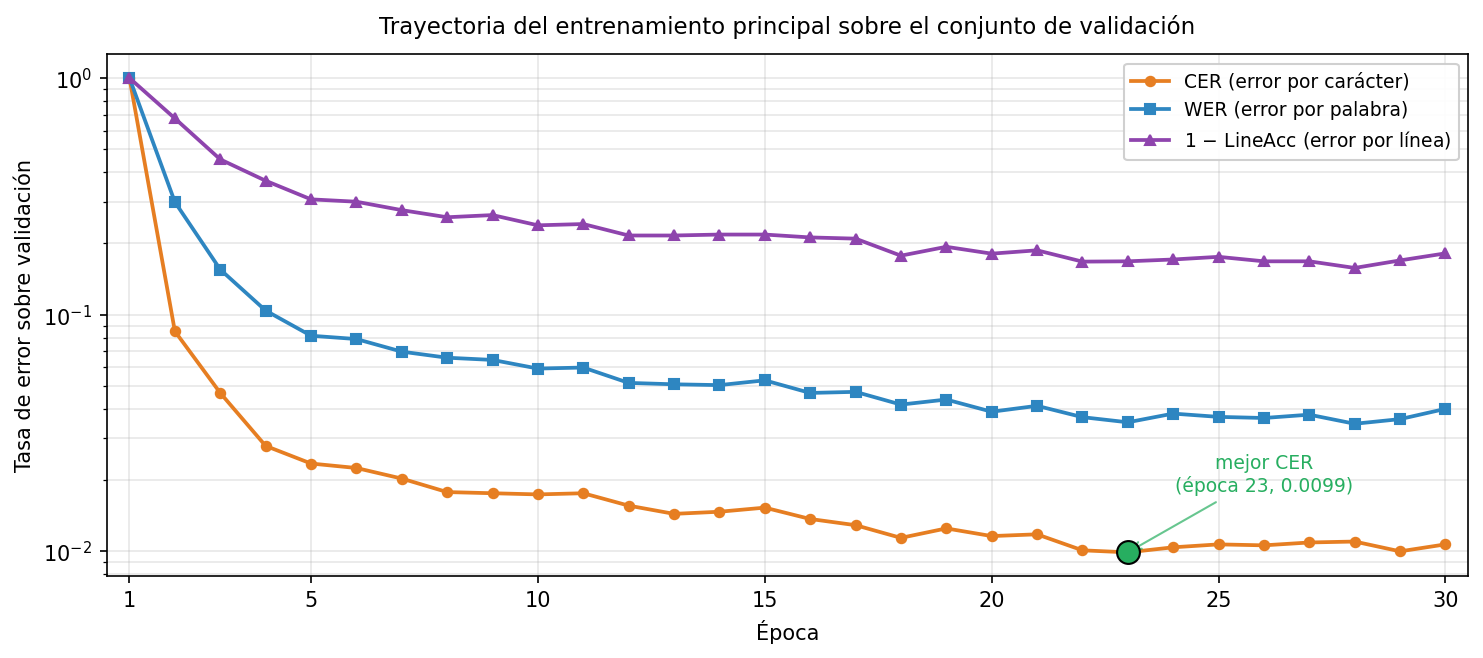
\includegraphics[width=\textwidth]{Graphics/curvas_entrenamiento.png}
	\caption{Trayectoria de las tres métricas de error sobre el conjunto de validación sintética con decodificación \textit{greedy}, a lo largo de las treinta épocas del entrenamiento principal: CER (error por carácter, en naranja), WER (error por palabra, en azul) y la tasa de error por línea, que resulta de restar la exactitud por línea a uno (en morado). Los tres ejes son escalas logarítmicas para que la caída inicial de tres órdenes de magnitud y el régimen estacionario posterior sean ambos legibles. El marcador verde señala la época veintitrés, donde el CER alcanza su valor mínimo de 0,0099 y de la cual procede el \textit{checkpoint} que producción emplea. La trayectoria conjunta de las tres métricas en el mismo eje permite contrastar la velocidad relativa de mejora de cada nivel de granularidad: el error por carácter cae más rápido y se estabiliza antes que el error por palabra, y este a su vez antes que el error por línea, lo que refleja la naturaleza multiplicativa de los errores a lo largo de una secuencia.}
	\label{fig:curvas-entrenamiento}
\end{figure}

La figura~\ref{fig:curvas-loss-lr} complementa la información anterior con la trayectoria de la pérdida CTC y del programador de tasa de aprendizaje a lo largo del entrenamiento. La pérdida de validación y la media por época de la pérdida de entrenamiento siguen trayectorias paralelas, con una separación que se mantiene por debajo de 0,02 unidades a lo largo del entrenamiento, lo que indica que el modelo no presenta sobreajuste medible al final de las treinta épocas. El programador \textit{OneCycleLR} eleva la tasa de aprendizaje desde un valor cercano a $10^{-5}$ en los primeros lotes hasta el máximo de $3 \times 10^{-4}$ en torno a la cuarta época, y la reduce de forma monótona hasta valores próximos a $10^{-8}$ en las últimas épocas para favorecer la convergencia del modelo.

\begin{figure}[!htbp]
	\centering
	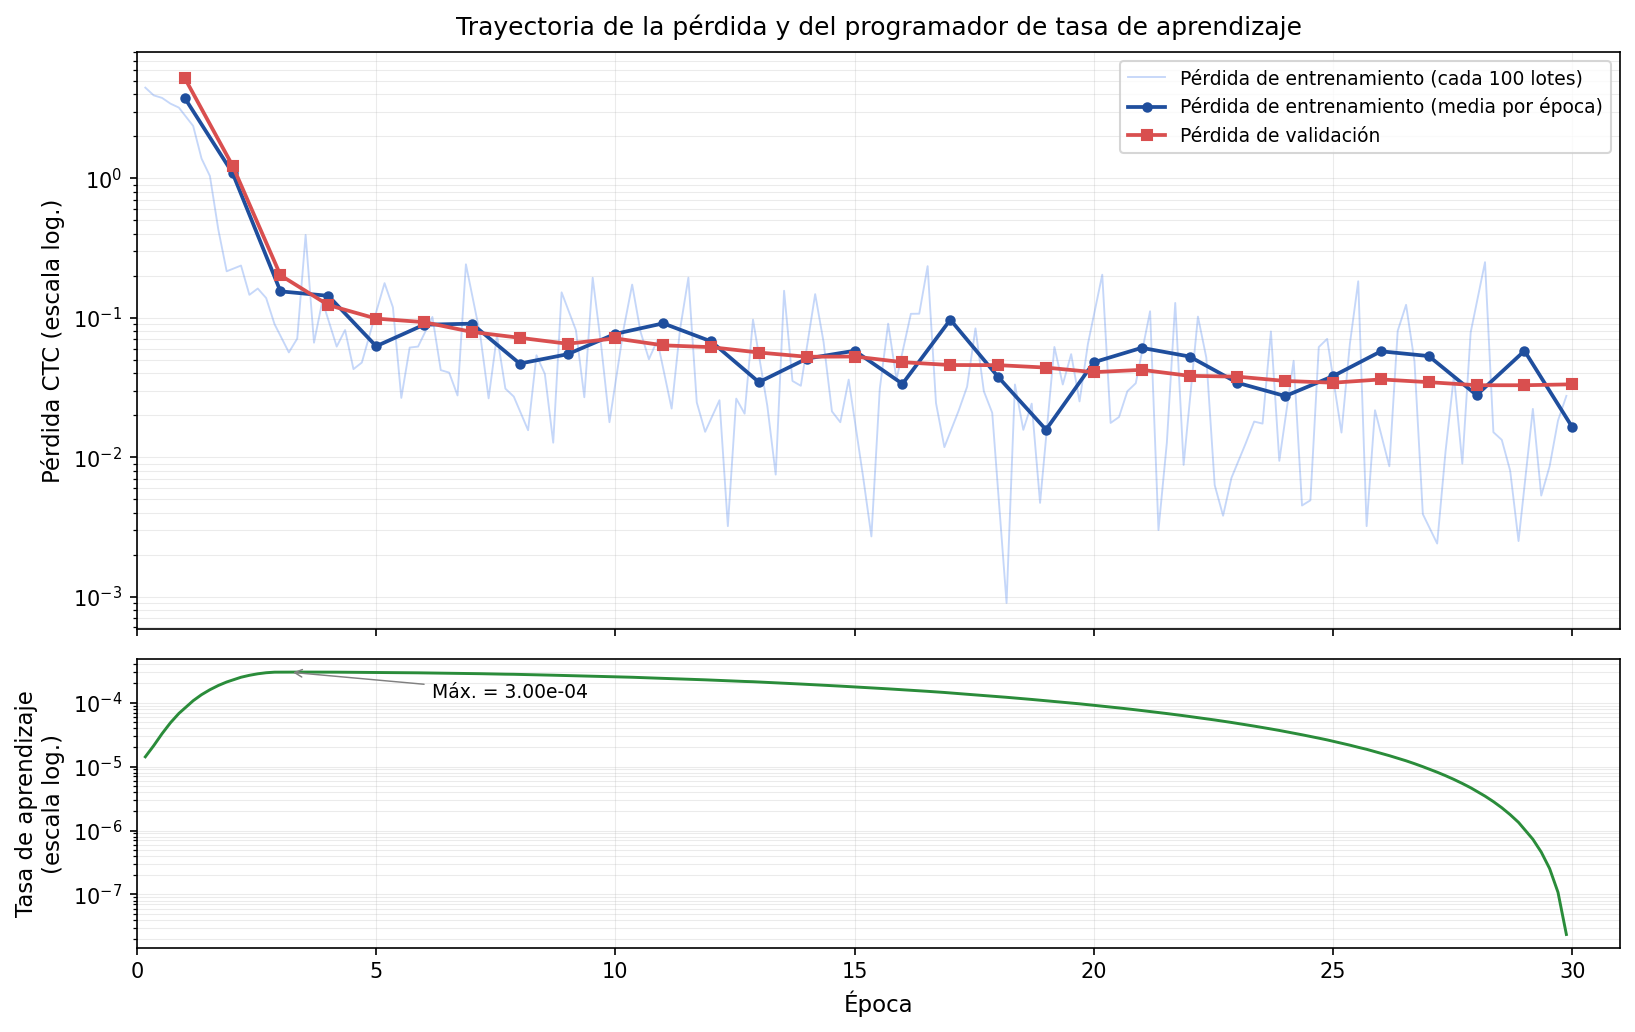
\includegraphics[width=\textwidth]{Graphics/curvas_loss_lr.png}
	\caption{Trayectoria de la pérdida CTC y del programador de tasa de aprendizaje a lo largo de las treinta épocas del entrenamiento principal. El panel superior reporta la pérdida de validación (línea roja con marcadores cuadrados), la media por época de la pérdida de entrenamiento (línea azul oscura con marcadores circulares) y la pérdida de entrenamiento por lote, muestreada cada cien lotes y representada en transparencia para no ocultar las medias. El panel inferior reporta la tasa de aprendizaje que el programador \textit{OneCycleLR} aplica a lo largo del entrenamiento. Los dos ejes verticales emplean escala logarítmica.}
	\label{fig:curvas-loss-lr}
\end{figure}

La pérdida cae más de dos órdenes de magnitud durante las primeras cinco épocas, y el modelo alcanza un CER inferior a 0,03 en la quinta época. A partir de la décima época la mejora se ralentiza y el CER oscila entre 0,01 y 0,02 hasta el final del entrenamiento. La tabla~\ref{tab:resultados-principal} resume las métricas que el modelo final alcanza con decodificación \textit{greedy} sobre el conjunto de validación, con intervalos de confianza al 95\,\% que el procedimiento \textit{bootstrap} produce.

\begin{table}[!htbp]
	\centering
	\caption{Resultados del entrenamiento principal sobre el conjunto de validación. La columna \emph{Std} reporta la desviación típica de la métrica por muestra; el procedimiento \textit{bootstrap} con diez mil remuestreos produce los intervalos de confianza al 95\,\%. La marcada asimetría de las distribuciones por muestra explica que la \emph{Std} alcance un orden de magnitud comparable o superior al de la media, ya que el modelo transcribe la mayoría de las líneas sin errores y un pequeño grupo concentra todos los errores. Esta asimetría justifica el recurso a tests no paramétricos.}
	\label{tab:resultados-principal}
	\begin{tabular}{lccc}
		\toprule
		\textbf{Métrica} & \textbf{Media} & \textbf{Std} & \textbf{IC 95\,\%} \\
		\midrule
		CER             & 0,0106 & 0,0374 & $[0{,}0090,\ 0{,}0122]$ \\
		WER             & 0,0374 & 0,1012 & $[0{,}0331,\ 0{,}0419]$ \\
		Exactitud por línea & 0,8269 & 0,3783 & $[0{,}8099,\ 0{,}8434]$ \\
		\bottomrule
	\end{tabular}
\end{table}

La tasa de error de carácter inferior al 1,1\,\% sitúa el sistema en un rango competitivo con los motores OCR para texto impreso en español, según discutió la sección~\ref{sec:estado-arte} del capítulo~\ref{chap:estado-arte}. La exactitud por línea próxima al 83\,\% indica que cuatro de cada cinco líneas reciben transcripción sin ningún error. La prueba binomial exacta sobre la exactitud por línea contrasta la hipótesis nula de un clasificador aleatorio con probabilidad 0,5 por línea frente a la alternativa de probabilidad superior, y la rechaza con un valor de probabilidad inferior a $10^{-200}$, lo que confirma la superioridad estadística del modelo sobre cualquier clasificador trivial.

El análisis por fuente tipográfica se resume en la tabla~\ref{tab:cer-por-fuente-principal}. La prueba de Kruskal-Wallis~\cite{kruskal1952ranks} sobre las nueve fuentes no rechaza la hipótesis de igualdad de distribuciones del CER entre fuentes, con $H = 11{,}93$ y valor de probabilidad $p = 0{,}154$. El resultado indica que el modelo no presenta un sesgo sistemático a favor de ninguna familia tipográfica del \textit{corpus} original.

\begin{table}[!htbp]
	\centering
	\caption{CER por fuente tipográfica sobre el conjunto de validación del entrenamiento principal. La columna \emph{Std} reporta la desviación típica del CER por muestra dentro de la fuente. Las nueve fuentes se ordenan alfabéticamente.}
	\label{tab:cer-por-fuente-principal}
	\begin{tabular}{lccc}
		\toprule
		\textbf{Fuente} & \textbf{CER} & \textbf{Std} & \textbf{IC 95\,\%} \\
		\midrule
		CourierPrime      & 0,0093 & 0,0405 & $[0{,}0047,\ 0{,}0152]$ \\
		CrimsonPro        & 0,0118 & 0,0375 & $[0{,}0071,\ 0{,}0171]$ \\
		CutiveMono        & 0,0083 & 0,0302 & $[0{,}0049,\ 0{,}0126]$ \\
		EBGaramond        & 0,0139 & 0,0424 & $[0{,}0088,\ 0{,}0199]$ \\
		Inconsolata       & 0,0101 & 0,0346 & $[0{,}0058,\ 0{,}0153]$ \\
		JetBrainsMono     & 0,0102 & 0,0401 & $[0{,}0057,\ 0{,}0157]$ \\
		LibreBaskerville  & 0,0119 & 0,0343 & $[0{,}0078,\ 0{,}0164]$ \\
		RobotoMono        & 0,0123 & 0,0460 & $[0{,}0072,\ 0{,}0187]$ \\
		SpecialElite      & 0,0076 & 0,0256 & $[0{,}0045,\ 0{,}0114]$ \\
		\bottomrule
	\end{tabular}
\end{table}

La validación cruzada estratificada por fuente que la subsección~\ref{subsec:cv-lofo} introduce permite cuantificar la sensibilidad del rendimiento frente a la partición aleatoria del \textit{corpus}. El protocolo divide las 19\,998 imágenes en cinco particiones que conservan la proporción de imágenes de cada fuente. Cada repetición entrena el modelo desde cero con cuatro particiones como entrenamiento y la quinta como validación, durante doce épocas. El número reducido de épocas respecto al entrenamiento principal mantiene el coste computacional total en un orden manejable y resulta suficiente para estimar la variabilidad de las métricas, que es el objetivo del experimento, sin necesidad de alcanzar el mejor modelo posible en cada repetición. La figura~\ref{fig:cv-5fold} presenta las trayectorias del CER por época sobre la partición de validación de cada repetición, junto con el CER final por partición.

\begin{figure}[!htbp]
	\centering
	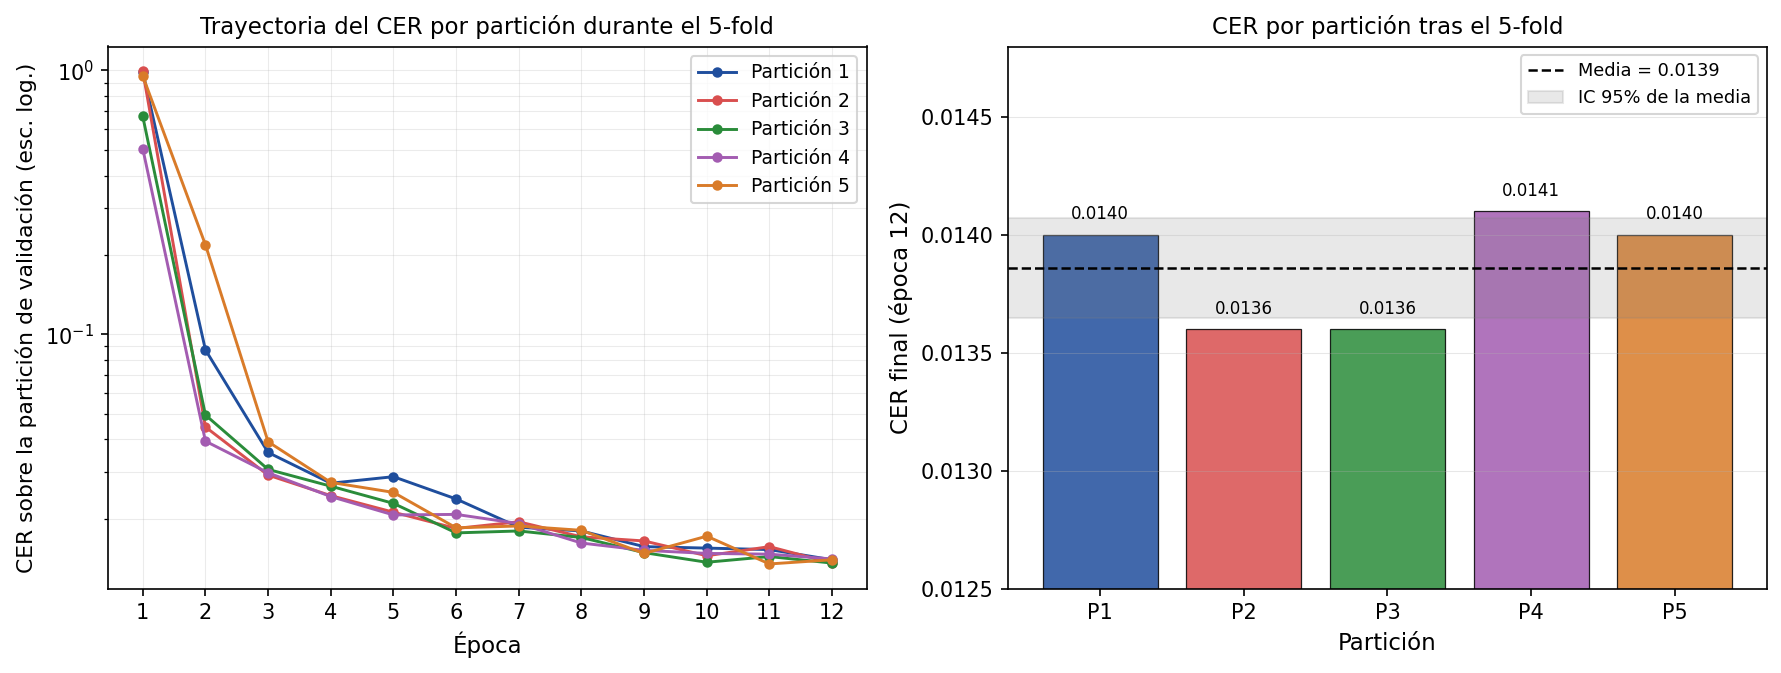
\includegraphics[width=\textwidth]{Graphics/cv_5fold.png}
	\caption{Validación cruzada de cinco particiones estratificadas por fuente. El panel izquierdo muestra la trayectoria del CER por época sobre la partición de validación correspondiente a cada repetición, en escala logarítmica. El panel derecho muestra el CER final tras doce épocas para cada partición, con la media (línea discontinua) y el intervalo de confianza al 95\,\% de la media (banda gris).}
	\label{fig:cv-5fold}
\end{figure}

El CER final de las cinco particiones cae en el intervalo $[0{,}0136;\ 0{,}0141]$, con media de 0,0138, desviación típica entre particiones de 0,00024 y coeficiente de variación de 1,7\,\%. La consistencia entre particiones indica que el rendimiento del modelo no depende de la partición aleatoria concreta del \textit{corpus}. La tabla~\ref{tab:cv-resumen} reporta el resumen agregado de las cinco métricas del protocolo de evaluación sobre las cinco repeticiones del experimento.

\begin{table}[!htbp]
	\centering
	\caption{Resumen agregado del experimento de validación cruzada de cinco particiones estratificadas por fuente. La columna \emph{Std} reporta la desviación típica entre particiones; las columnas \emph{Mín} y \emph{Máx} reportan el rango observado; la columna \emph{IC 95\,\%} reporta el intervalo de confianza al 95\,\% de la media de las cinco mediciones.}
	\label{tab:cv-resumen}
	\begin{tabular}{lccccc}
		\toprule
		\textbf{Métrica} & \textbf{Media} & \textbf{Std} & \textbf{Mín} & \textbf{Máx} & \textbf{IC 95\,\%} \\
		\midrule
		CER                  & 0,0138 & 0,00024 & 0,0135 & 0,0141 & $[0{,}0135,\ 0{,}0140]$ \\
		WER                  & 0,0490 & 0,00111 & 0,0472 & 0,0506 & $[0{,}0477,\ 0{,}0504]$ \\
		Exactitud por línea  & 0,7891 & 0,00653 & 0,7802 & 0,7991 & $[0{,}7810,\ 0{,}7972]$ \\
		Char-F1              & 0,9892 & 0,00022 & 0,9889 & 0,9895 & $[0{,}9890,\ 0{,}9895]$ \\
		BLEU-4 (carácter)    & 0,9746 & 0,00054 & 0,9738 & 0,9752 & $[0{,}9739,\ 0{,}9752]$ \\
		\bottomrule
	\end{tabular}
\end{table}

Los valores de la tabla~\ref{tab:cv-resumen} son sistemáticamente menos favorables que los del entrenamiento principal porque cada repetición de la validación cruzada entrena el modelo durante doce épocas sobre cuatro quintas partes del \textit{corpus}, frente a treinta épocas sobre nueve décimas partes del \textit{corpus} del entrenamiento principal. La comparación pertinente entre los dos protocolos no se refiere al nivel absoluto del CER sino a su variabilidad: la desviación típica del CER entre particiones, equivalente al 1,7\,\% de la media, confirma que el rendimiento del modelo no es accidente de una partición concreta.

El experimento LOFO produjo un CER promedio sobre las fuentes que quedan fuera de 0,0192, con intervalo de confianza al 95\,\% de $[0{,}0125,\ 0{,}0259]$. La degradación respecto al CER \textit{in-sample} de 0,0106 fue de 0,0086, valor inferior al umbral de 0,05 que el protocolo considera tolerable. La figura~\ref{fig:lofo-por-fuente} compara, para cada una de las nueve fuentes, el CER \textit{in-sample} (cuando la fuente sí participó en el entrenamiento) frente al CER LOFO (cuando la fuente quedó fuera).

\begin{figure}[!htbp]
	\centering
	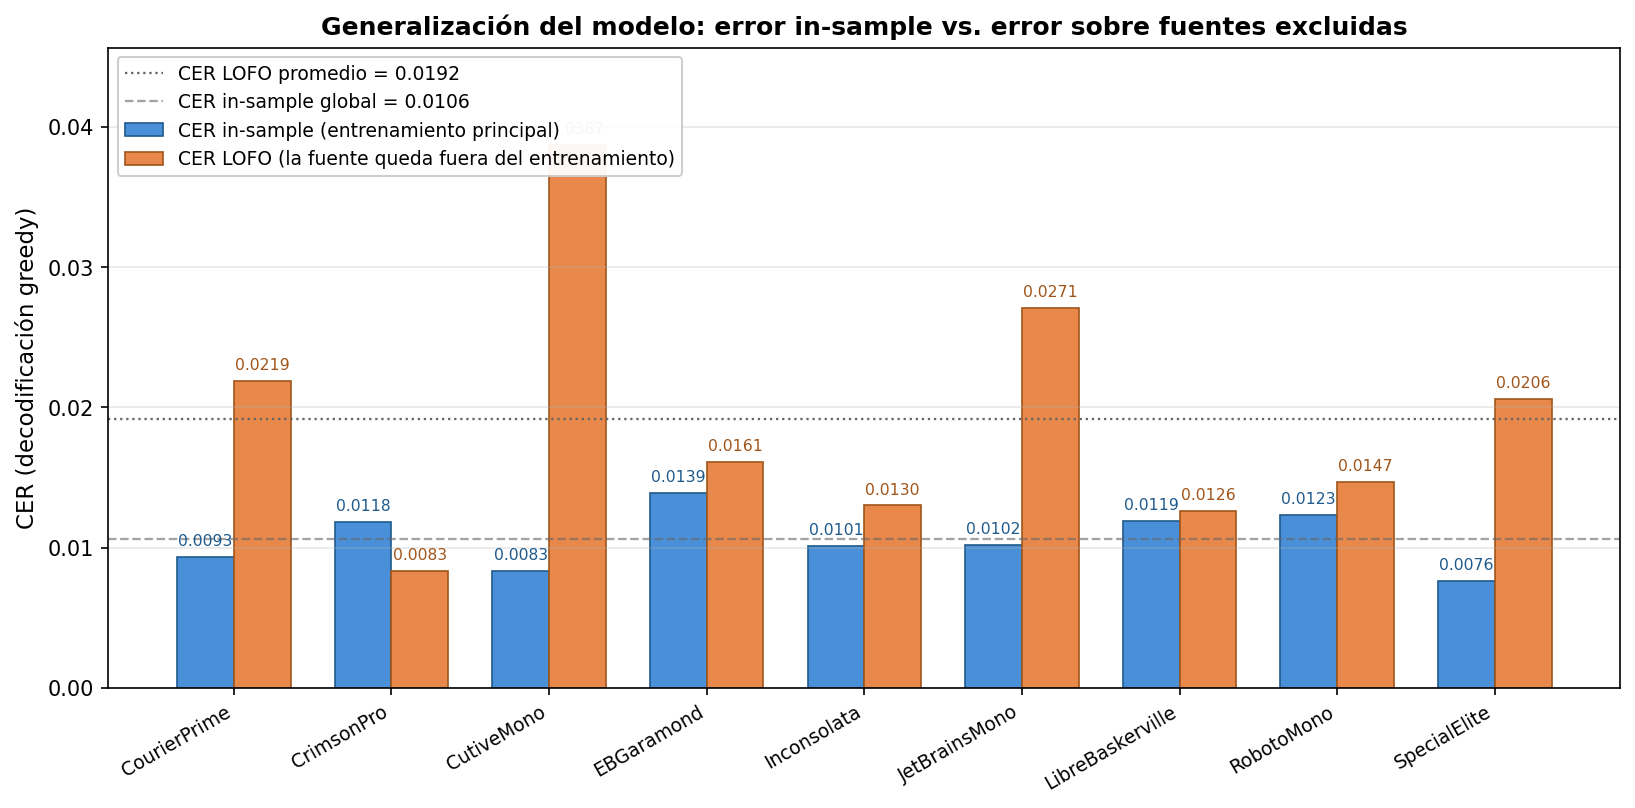
\includegraphics[width=\textwidth]{Graphics/lofo_por_fuente.png}
	\caption{Comparación del CER \textit{in-sample} (azul) y el CER LOFO (naranja) para cada una de las nueve fuentes del \textit{corpus} original. La línea discontinua marca el CER \textit{in-sample} global (0,0106) y la línea punteada marca el CER LOFO promedio (0,0192). La fuente con menor degradación es CrimsonPro y la fuente con mayor degradación es CutiveMono.}
	\label{fig:lofo-por-fuente}
\end{figure}

El comportamiento es marcadamente heterogéneo. CrimsonPro, LibreBaskerville e Inconsolata muestran degradaciones inferiores a 0,003 puntos, lo que indica que el modelo aprende a leerlas adecuadamente a partir de las restantes fuentes serif o monoespaciadas del \textit{corpus}. En el extremo opuesto, CutiveMono pasa de un CER \textit{in-sample} de 0,0083 a un CER LOFO de 0,0387, lo que sugiere que esta tipografía presenta rasgos que las restantes fuentes del \textit{corpus} cubren mal. JetBrainsMono y SpecialElite siguen patrones intermedios.

% -----------------------------------------------------------------------------
\section{Adaptación mediante \textit{fine-tuning}}
\label{sec:fine-tuning}

La etapa de \textit{fine-tuning} parte del modelo de la fase principal y continúa el entrenamiento sobre un \textit{corpus} con seis fuentes tipográficas adicionales. La ampliación responde a una observación práctica: durante la evaluación del modelo sobre documentos de prueba con tipografías serif que el entrenamiento principal no cubría, el equipo detectó errores sistemáticos sobre caracteres con remates que las tres serif del \textit{corpus} original representaban poco. La ampliación del repertorio tipográfico es la respuesta directa al objetivo, que el capítulo~\ref{chap:intro} declara, de maximizar la generalización del modelo frente a tipografías arbitrarias.

Las seis fuentes que el corpus extendido añade son Lora, Merriweather, Palatino, SourceSerif4, Georgia y Times. El conjunto refuerza la familia serif del \textit{corpus} original con tipografías de uso amplio en publicaciones modernas y en sistemas operativos comerciales. La generación del \textit{corpus} extendido sigue el procedimiento que el capítulo~\ref{chap:corpus} describe, con la única diferencia del catálogo tipográfico.

\subsection{Análisis exploratorio del \textit{corpus} extendido}
\label{subsec:eda-extendido}

El \textit{corpus} extendido pasa por el mismo procedimiento de análisis exploratorio que la sección~\ref{sec:eda-corpus} del capítulo~\ref{chap:corpus} aplicó al \textit{corpus} de entrenamiento. La caracterización del \textit{corpus} extendido es necesaria para confirmar que las propiedades de diseño que sostienen la generación se mantienen tras la ampliación del catálogo tipográfico, y para verificar que las nuevas fuentes siguen cumpliendo la restricción de la función de pérdida CTC. La figura~\ref{fig:eda-dashboard-extendido} reúne las visualizaciones del análisis.

\begin{figure}[!htbp]
	\centering
	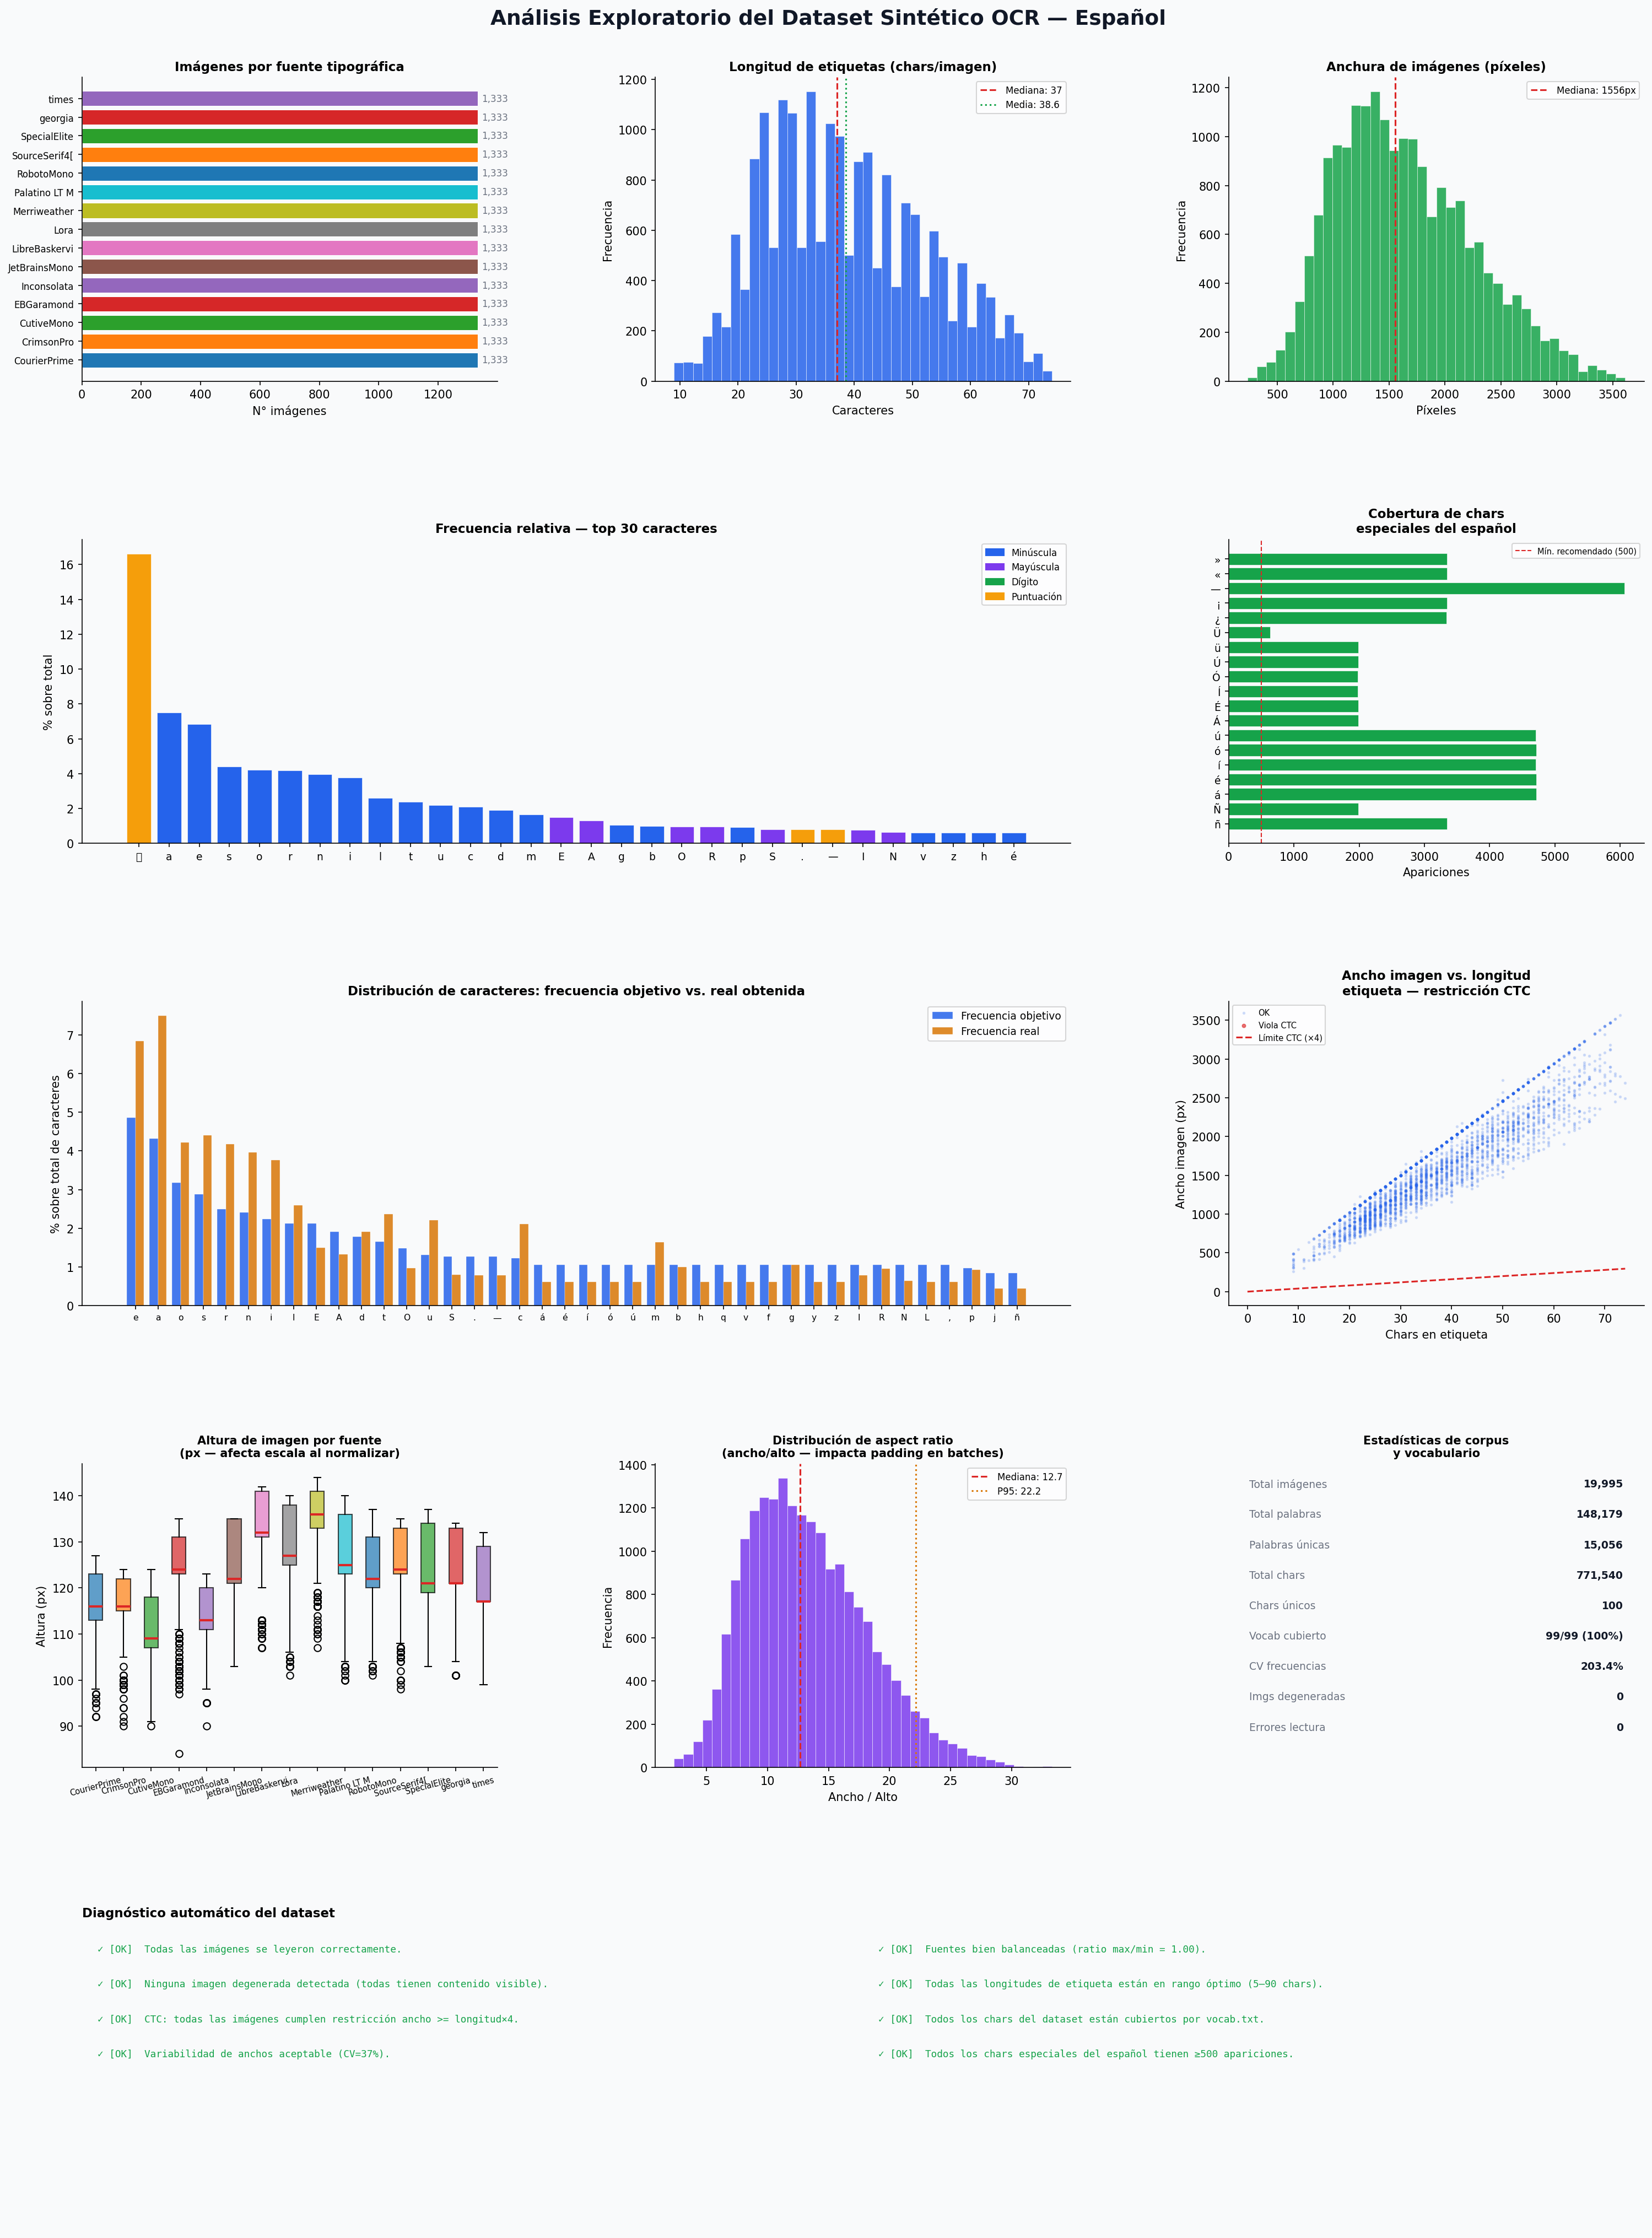
\includegraphics[width=0.85\textwidth]{Graphics/eda_dashboard_extendido.png}
	\caption{Análisis exploratorio del \textit{corpus} sintético extendido para la etapa de \textit{fine-tuning}, con 19\,995 imágenes que el generador produce a partir de las quince fuentes tipográficas (las nueve del \textit{corpus} original más las seis que se añaden en esta etapa). El panel reúne las distribuciones de imágenes por fuente, longitudes de etiqueta, anchos, frecuencias de caracteres, cobertura del vocabulario español, cumplimiento de la restricción CTC, alturas por fuente y aspect ratio de las imágenes.}
	\label{fig:eda-dashboard-extendido}
\end{figure}

El \textit{corpus} extendido reúne 19\,995 imágenes con un reparto perfectamente uniforme entre las quince fuentes, 1\,333 imágenes por cada una, y cociente máximo--mínimo igual a la unidad. La reducción de la cuota por fuente respecto al \textit{corpus} original, donde cada fuente aportaba 2\,222 imágenes, es la consecuencia directa de mantener el tamaño global del \textit{corpus} constante mientras el catálogo tipográfico crece. La decisión de no aumentar el volumen global respeta la práctica habitual del \textit{fine-tuning}, que opera con cantidades de datos del mismo orden que el entrenamiento principal y no requiere ampliar el volumen agregado.

Las longitudes de etiqueta presentaron media de 38,6 caracteres, mediana de 37, rango entre 9 y 74 y desviación típica de 13,8, con percentiles 5, 25, 75 y 95 en 19, 28, 48 y 64 caracteres, respectivamente. Los valores reproducen casi exactamente la distribución del \textit{corpus} original, lo que indica que el algoritmo de generación de cadenas balanceadas que el capítulo~\ref{chap:corpus} describe es robusto frente al cambio del repertorio tipográfico.

Las dimensiones de imagen presentaron media de ancho de 1\,639 píxeles, mediana de 1\,556 píxeles, rango entre 234 y 3\,612 píxeles y coeficiente de variación del 37,5\,\%. La media de altura fue de 123 píxeles, con rango entre 84 y 144 píxeles. La pequeña reducción del ancho medio respecto al \textit{corpus} original (1\,704 píxeles) refleja la incorporación de fuentes serif modernas con paso tipográfico más compacto que las monoespacio dominantes del \textit{corpus} original. La verificación de la restricción CTC sobre el \textit{corpus} extendido confirmó que ninguna de las 19\,995 imágenes la viola, en línea con el resultado equivalente sobre el \textit{corpus} de entrenamiento.

La cobertura del vocabulario fue total: el \textit{corpus} extendido contiene los cien símbolos del vocabulario del sistema. El \textit{corpus} reúne 771\,540 caracteres en 148\,179 palabras, de las cuales 15\,056 son únicas. El coeficiente de variación de las frecuencias de caracteres alcanzó el 203,4\,\%, valor casi idéntico al del \textit{corpus} original y consistente con la ley de Zipf del lenguaje natural. Los caracteres específicos del español formal mantienen todos la cobertura por encima del umbral mínimo de 500 apariciones, con la eñe en 3\,348 apariciones, las comillas angulares en 3\,346 y 3\,343, la raya de diálogo en 6\,061 y los signos de apertura de interrogación y exclamación por encima de 3\,300 cada uno. Tres símbolos genéricos quedan por debajo del umbral, los mismos que en el \textit{corpus} original: el corchete derecho (89 apariciones), el corchete izquierdo (85) y la almohadilla (81). El criterio que la sección~\ref{sec:eda-corpus} expuso aplica también aquí: los tres no figuran entre los caracteres específicos del español y la cobertura mínima del vocabulario del idioma resulta satisfactoria.

El análisis exploratorio confirma que el \textit{corpus} extendido conserva todas las propiedades de diseño del \textit{corpus} original: uniformidad entre fuentes, distribución de longitudes en rango operativo, cobertura completa del vocabulario, todos los caracteres del español por encima del umbral mínimo, y respeto de la restricción CTC. La única diferencia, por diseño, está en la cuota por fuente, que disminuye a la mitad por el incremento del catálogo de nueve a quince fuentes. La caracterización valida el \textit{corpus} extendido como entrada apta para la etapa de \textit{fine-tuning}.

\subsection{Protocolo de \textit{fine-tuning}}
\label{subsec:protocolo-finetune}

El protocolo de \textit{fine-tuning} reutiliza la configuración del entrenamiento principal con las diferencias que la tabla~\ref{tab:diff-finetune} resume.

\begin{table}[!htbp]
	\centering
	\caption{Diferencias de configuración entre el entrenamiento principal y la etapa de \textit{fine-tuning}.}
	\label{tab:diff-finetune}
	\scriptsize
	\begin{tabular}{lcc}
		\toprule
		\textbf{Hiperparámetro} & \textbf{Entrenamiento principal} & \textbf{\textit{Fine-tuning}} \\
		\midrule
		Punto de partida & pesos inicializados (Xavier) & mejor \textit{checkpoint} de la fase principal \\
		Épocas & 30 & 20 \\
		Tasa de aprendizaje máxima & $3 \times 10^{-4}$ & $5 \times 10^{-5}$ \\
		Recorte de gradiente (norma máx.) & 5,0 & 3,0 \\
		Catálogo tipográfico (fuentes) & 9 & 15 \\
		\bottomrule
	\end{tabular}
\end{table}

La reducción de la tasa de aprendizaje a aproximadamente un sexto y la del recorte de gradiente reflejan la práctica habitual de continuación desde un punto de control preentrenado: el modelo parte ya de una buena solución y conviene evitar pasos demasiado grandes que la destruyan. El conjunto de hiperparámetros restante coincide con el del entrenamiento principal. La figura~\ref{fig:curvas-finetuning} muestra la trayectoria de las tres métricas de error sobre el conjunto de validación a lo largo de las veinte épocas del \textit{fine-tuning}.

\begin{figure}[!htbp]
	\centering
	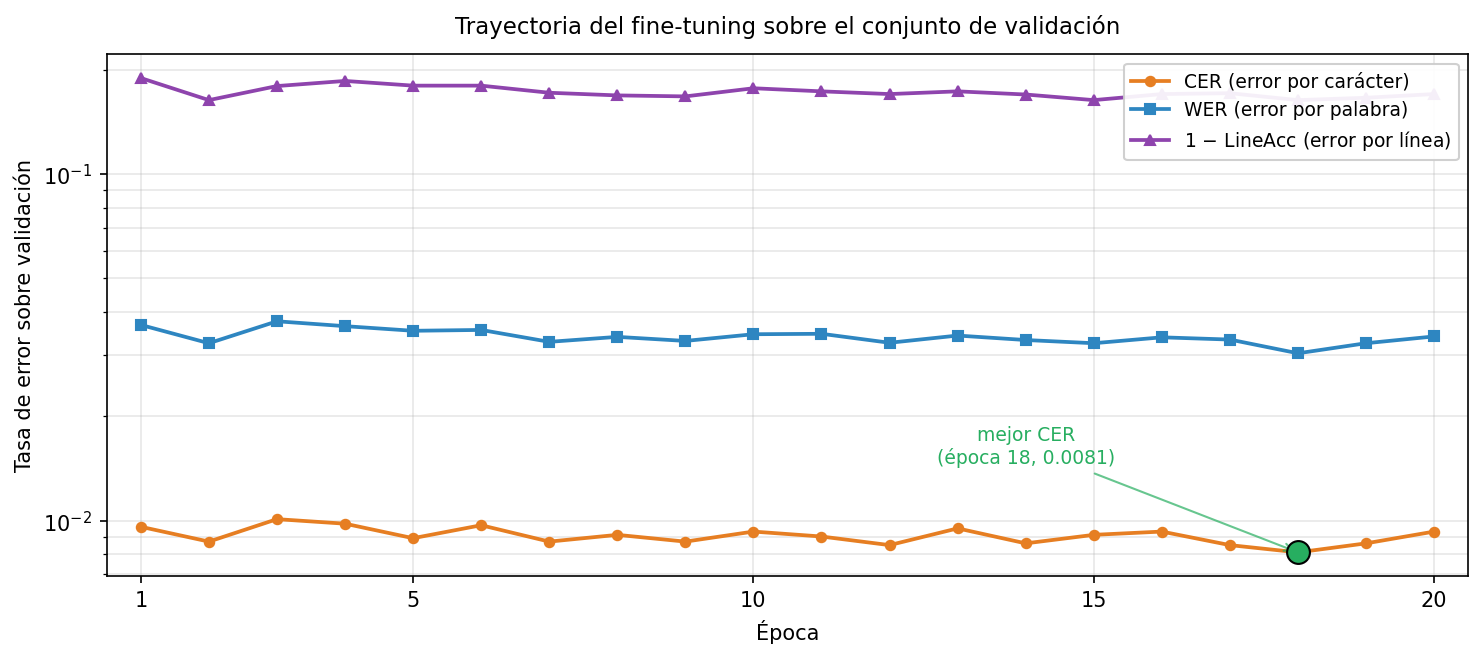
\includegraphics[width=\textwidth]{Graphics/curvas_finetuning.png}
	\caption{Trayectoria de las tres métricas de error sobre el conjunto de validación sintética con decodificación \textit{greedy}, a lo largo de las veinte épocas del \textit{fine-tuning} sobre el \textit{corpus} extendido. El eje vertical, en escala logarítmica, comparte el rango con la figura~\ref{fig:curvas-entrenamiento} del entrenamiento principal para facilitar la comparación visual. El régimen es estacionario desde la primera época, con oscilaciones en un entorno cerrado en torno a CER 0,009, WER 0,034 y tasa de error por línea 0,17. La ausencia de tendencia descendente es esperable, ya que el \textit{fine-tuning} parte del mejor \textit{checkpoint} del entrenamiento principal, que el modelo no podía mejorar de forma apreciable sin un cambio de dominio o de capacidad. El marcador verde señala el mejor CER, que el modelo alcanza en la época dieciocho con valor 0,0081.}
	\label{fig:curvas-finetuning}
\end{figure}

La tabla~\ref{tab:comparativa-finetune} compara las métricas globales antes y después del \textit{fine-tuning}.

\begin{table}[!htbp]
	\centering
	\caption{Métricas globales antes y después del \textit{fine-tuning} sobre el conjunto de validación correspondiente. La columna de variación reporta la reducción porcentual sobre el CER y el WER.}
	\label{tab:comparativa-finetune}
	\begin{tabular}{lccc}
		\toprule
		\textbf{Métrica} & \textbf{Principal (9 fuentes)} & \textbf{\textit{Fine-tuning} (15 fuentes)} & \textbf{Variación} \\
		\midrule
		CER             & 0,0106 & 0,0088 & $-17{,}\%$ \\
		WER             & 0,0374 & 0,0331 & $-12{,}\%$ \\
		Exactitud por línea & 0,8269 & 0,8304 & $+0{,}35$~pp \\
		\bottomrule
	\end{tabular}
\end{table}

El modelo final, sobre la validación extendida de quince fuentes, alcanza un CER del 0{,}88\,\%, valor consistente con el rango del entrenamiento principal sobre las nueve fuentes originales (CER del 1{,}06\,\%). Las dos cifras corresponden a distribuciones de validación distintas y una comparación isodistribuida estricta exigiría medir el modelo principal sobre la validación extendida; la subsección~\ref{subsec:lofo-post-ft} reporta la comparación rigurosa entre ambos modelos sobre un mismo protocolo experimental, que cuantifica el efecto del \textit{fine-tuning} sobre la generalización tipográfica. La prueba de Kruskal-Wallis sobre las quince fuentes del \textit{corpus} extendido no rechaza la hipótesis de igualdad de distribuciones entre fuentes ($H = 17{,}04$, $p = 0{,}254$), lo que indica que el modelo, tras el \textit{fine-tuning}, alcanza una uniformidad de rendimiento entre fuentes consistente con la del entrenamiento original. La tabla~\ref{tab:cer-por-fuente-finetune} reporta el CER de cada una de las quince fuentes.

\begin{table}[!htbp]
	\centering
	\caption{CER por fuente tipográfica tras el \textit{fine-tuning} sobre el \textit{corpus} extendido. La columna \emph{Std} reporta la desviación típica del CER por muestra dentro de la fuente. Las seis fuentes que se añaden en esta etapa aparecen en negrita.}
	\label{tab:cer-por-fuente-finetune}
	\begin{tabular}{lccc}
		\toprule
		\textbf{Fuente} & \textbf{CER} & \textbf{Std} & \textbf{IC 95\,\%} \\
		\midrule
		CourierPrime      & 0,0125 & 0,0387 & $[0{,}0065,\ 0{,}0200]$ \\
		CrimsonPro        & 0,0042 & 0,0125 & $[0{,}0022,\ 0{,}0066]$ \\
		CutiveMono        & 0,0062 & 0,0205 & $[0{,}0031,\ 0{,}0100]$ \\
		EBGaramond        & 0,0095 & 0,0233 & $[0{,}0062,\ 0{,}0135]$ \\
		Inconsolata       & 0,0122 & 0,0393 & $[0{,}0064,\ 0{,}0191]$ \\
		JetBrainsMono     & 0,0134 & 0,0454 & $[0{,}0068,\ 0{,}0223]$ \\
		LibreBaskerville  & 0,0067 & 0,0236 & $[0{,}0031,\ 0{,}0114]$ \\
		\textbf{Lora}     & 0,0080 & 0,0252 & $[0{,}0038,\ 0{,}0127]$ \\
		\textbf{Merriweather} & 0,0090 & 0,0459 & $[0{,}0025,\ 0{,}0184]$ \\
		\textbf{Palatino} & 0,0106 & 0,0420 & $[0{,}0045,\ 0{,}0192]$ \\
		RobotoMono        & 0,0106 & 0,0367 & $[0{,}0054,\ 0{,}0177]$ \\
		\textbf{SourceSerif4} & 0,0053 & 0,0153 & $[0{,}0028,\ 0{,}0083]$ \\
		SpecialElite      & 0,0064 & 0,0234 & $[0{,}0030,\ 0{,}0109]$ \\
		\textbf{Georgia}  & 0,0097 & 0,0291 & $[0{,}0055,\ 0{,}0154]$ \\
		\textbf{Times}    & 0,0072 & 0,0291 & $[0{,}0031,\ 0{,}0130]$ \\
		\bottomrule
	\end{tabular}
\end{table}

El análisis de los errores de carácter más frecuentes que el modelo final produce identifica dos patrones predominantes. El primero es la confusión entre signos de puntuación visualmente similares, con la coma que el modelo confunde con el punto como el error más frecuente. El segundo es la omisión de tildes, que confunde la vocal con tilde con su contrapartida sin tilde. Los dos patrones son consistentes con la dificultad de los caracteres que intervienen, que difieren por rasgos de pocos píxeles en tipografías de cuerpo pequeño.

% -----------------------------------------------------------------------------
\section{Evaluación final sobre el conjunto de prueba}
\label{sec:test-set}

La evaluación final del sistema descansa sobre un conjunto de prueba independiente que el protocolo reserva para una única medición, después de la etapa de \textit{fine-tuning} que la sección~\ref{sec:fine-tuning} describe. La medición sobre este conjunto constituye la estimación insesgada del rendimiento del modelo desplegado: el conjunto de prueba no participa en la selección del \textit{checkpoint}, no contribuye a las decisiones de hiperparámetros y el desarrollo no lo observa más de una vez.

La decisión de aplicar la evaluación final únicamente después del \textit{fine-tuning}, y no al término del entrenamiento principal, responde a dos consideraciones metodológicas. La primera es que el modelo que el sistema despliega corresponde al modelo posterior al \textit{fine-tuning}; una evaluación intermedia tras el entrenamiento principal habría producido la métrica de un modelo que no llega a producción, sin valor operativo para los resultados que el documento reporta. La segunda es que reutilizar el conjunto de prueba en dos momentos del desarrollo, uno tras el entrenamiento principal y otro tras el \textit{fine-tuning}, habría introducido un sesgo de selección sobre la decisión misma de continuar con la adaptación: la observación del primer número habría podido influir en el resto del proceso, lo que invalidaría la segunda medición como estimador insesgado. La política de uso único del conjunto de prueba es la práctica habitual en aprendizaje automático precisamente por esta razón. Durante el desarrollo, la validación cruzada estratificada por fuente y el experimento de exclusión de una fuente que la subsección~\ref{subsec:cv-lofo} describe cumplieron el papel de cuantificación de la generalización sin consumir el presupuesto del conjunto de prueba.

\subsection{Composición del conjunto de prueba}
\label{subsec:test-composicion}

El generador del \textit{corpus} produjo 1\,995 imágenes a partir de las quince fuentes tipográficas del repertorio extendido, con un reparto perfectamente uniforme de 133 imágenes por fuente y un cociente entre la frecuencia máxima y la mínima igual a la unidad. El procedimiento de generación es idéntico al que el capítulo~\ref{chap:corpus} describe para el \textit{corpus} de entrenamiento, con una sola diferencia: la semilla aleatoria que controla el muestreo de cadenas a partir del \textit{corpus} textual de Project Gutenberg toma un valor distinto del que la generación del \textit{corpus} de entrenamiento empleó. El cambio de semilla garantiza por construcción que ninguna cadena del conjunto de prueba coincida con una del entrenamiento o la validación. La longitud media de las cadenas del conjunto de prueba es de 38,7 caracteres, en línea con la del \textit{corpus} de entrenamiento que el capítulo~\ref{chap:corpus} reporta.

\subsection{Resultados globales}
\label{subsec:test-global}

La tabla~\ref{tab:test-global} reporta las métricas principales sobre el conjunto de prueba con decodificación \textit{greedy} sobre el modelo final tras el \textit{fine-tuning}, con intervalos de confianza al 95\,\% por \textit{bootstrap} con diez mil remuestreos.

\begin{table}[!htbp]
	\centering
	\caption{Resultados del modelo final sobre el conjunto de prueba independiente de 1\,995 imágenes. Decodificación \textit{greedy} sobre el modelo posterior a la etapa de \textit{fine-tuning}. El procedimiento \textit{bootstrap} con diez mil remuestreos produce los intervalos de confianza al 95\,\%. La métrica BLEU-4 es una métrica agregada del conjunto y no admite intervalo de confianza por remuestreo de muestras individuales.}
	\label{tab:test-global}
	\begin{tabular}{lccc}
		\toprule
		\textbf{Métrica}     & \textbf{Media} & \textbf{Std} & \textbf{IC 95\,\%} \\
		\midrule
		CER                  & 0,0428 & 0,0469 & $[0{,}0407,\ 0{,}0448]$ \\
		WER                  & 0,0973 & 0,1333 & $[0{,}0916,\ 0{,}1032]$ \\
		Exactitud por línea  & 0,3739 & 0,4840 & $[0{,}3524,\ 0{,}3950]$ \\
		Char-F1              & 0,9793 & 0,0222 & $[0{,}9783,\ 0{,}9803]$ \\
		BLEU-4 (carácter)    & 0,9625 & ---    & --- \\
		\bottomrule
	\end{tabular}
\end{table}

El CER del 4,28\,\% sobre el conjunto de prueba es superior al CER del 0,88\,\% que el conjunto de validación reportó tras el \textit{fine-tuning}. Tres factores combinados explican la diferencia. El primero es la selección del \textit{checkpoint} durante el entrenamiento: el protocolo guarda en cada época el modelo con menor CER sobre validación, lo que introduce un sesgo optimista sobre la métrica de validación. El segundo es el origen de las cadenas: el protocolo obtiene el conjunto de validación por partición aleatoria del \textit{corpus} de entrenamiento, mientras que el conjunto de prueba parte de un muestreo independiente del mismo \textit{corpus} textual de Project Gutenberg con una semilla distinta, lo que produce material léxico que el modelo no encontró durante el entrenamiento. El tercero es la política de uso único: el protocolo evalúa el conjunto de prueba una sola vez sobre el modelo final, sin posibilidad de selección posterior. La estimación de prueba constituye, por estos tres motivos, el indicador insesgado del rendimiento que cabe esperar del modelo en condiciones operativas sobre material sintético comparable. El CER del 4,28\,\% sitúa al sistema en un rango competitivo con los motores OCR para texto impreso en español según la discusión del estado del arte que el capítulo~\ref{chap:estado-arte} ofrece, y la exactitud por línea próxima al 37\,\% indica que más de una de cada tres líneas recibe transcripción sin error alguno.

\subsection{Resultados por fuente tipográfica}
\label{subsec:test-por-fuente}

La tabla~\ref{tab:test-por-fuente} reporta el CER, la desviación típica del CER por muestra, la exactitud por línea y el intervalo de confianza al 95\,\% sobre el CER, para cada una de las quince fuentes del conjunto de prueba.

\begin{table}[!htbp]
	\centering
	\caption{CER, desviación típica del CER por muestra, exactitud por línea e intervalo de confianza al 95\,\% sobre el CER por fuente tipográfica, sobre el conjunto de prueba de 1\,995 imágenes (133 por fuente). Decodificación \textit{greedy} sobre el modelo final tras \textit{fine-tuning}. Las seis fuentes en negrita son las que el \textit{fine-tuning} añadió al \textit{corpus} original.}
	\label{tab:test-por-fuente}
	\begin{tabular}{lcccc}
		\toprule
		\textbf{Fuente} & \textbf{CER} & \textbf{Std} & \textbf{LineAcc} & \textbf{IC 95\,\%} \\
		\midrule
		CourierPrime          & 0,0214 & 0,0315 & 0,5940 & $[0{,}0163,\ 0{,}0268]$ \\
		CrimsonPro            & 0,0556 & 0,0530 & 0,3008 & $[0{,}0469,\ 0{,}0646]$ \\
		CutiveMono            & 0,0170 & 0,0309 & 0,6541 & $[0{,}0120,\ 0{,}0225]$ \\
		EBGaramond            & 0,0597 & 0,0579 & 0,2632 & $[0{,}0501,\ 0{,}0698]$ \\
		Inconsolata           & 0,0291 & 0,0424 & 0,5188 & $[0{,}0223,\ 0{,}0366]$ \\
		JetBrainsMono         & 0,0200 & 0,0275 & 0,5489 & $[0{,}0156,\ 0{,}0248]$ \\
		LibreBaskerville      & 0,0422 & 0,0422 & 0,3233 & $[0{,}0354,\ 0{,}0496]$ \\
		\textbf{Lora}         & 0,0572 & 0,0457 & 0,2180 & $[0{,}0497,\ 0{,}0651]$ \\
		\textbf{Merriweather} & 0,0552 & 0,0493 & 0,2632 & $[0{,}0469,\ 0{,}0635]$ \\
		\textbf{Palatino}     & 0,0514 & 0,0468 & 0,3008 & $[0{,}0437,\ 0{,}0594]$ \\
		RobotoMono            & 0,0167 & 0,0280 & 0,6316 & $[0{,}0122,\ 0{,}0215]$ \\
		\textbf{SourceSerif4} & 0,0514 & 0,0510 & 0,3308 & $[0{,}0430,\ 0{,}0602]$ \\
		SpecialElite          & 0,0521 & 0,0550 & 0,2406 & $[0{,}0434,\ 0{,}0621]$ \\
		\textbf{Georgia}      & 0,0601 & 0,0461 & 0,1880 & $[0{,}0524,\ 0{,}0681]$ \\
		\textbf{Times}        & 0,0523 & 0,0404 & 0,2331 & $[0{,}0456,\ 0{,}0593]$ \\
		\bottomrule
	\end{tabular}
\end{table}

La prueba de Kruskal-Wallis~\cite{kruskal1952ranks} sobre el CER entre las quince fuentes rechaza la hipótesis de igualdad de distribuciones con $H = 280{,}90$ y un valor de probabilidad inferior a $10^{-50}$. El rechazo contrasta con el resultado de las pruebas equivalentes sobre los conjuntos de validación del entrenamiento principal ($H = 11{,}93$, $p = 0{,}154$) y del \textit{fine-tuning} ($H = 17{,}04$, $p = 0{,}254$) que las secciones~\ref{sec:resultados-entrenamiento} y~\ref{sec:fine-tuning} reportan, y refleja que la evaluación sobre material léxico independiente del entrenamiento expone diferencias sistemáticas de dificultad entre familias tipográficas que la evaluación sobre material léxico compartido enmascara.

El comportamiento por fuente sigue un patrón coherente con la estructura del catálogo tipográfico. Las cinco fuentes monoespaciadas (CourierPrime, CutiveMono, Inconsolata, JetBrainsMono y RobotoMono) alcanzan los CER más bajos del rango, entre 0,0167 y 0,0291, y exactitudes por línea entre el 52\,\% y el 66\,\%. Las nueve fuentes serif, tanto las del \textit{corpus} original (CrimsonPro, EBGaramond y LibreBaskerville) como las seis que el \textit{fine-tuning} incorporó (Lora, Merriweather, Palatino, SourceSerif4, Georgia y Times), junto con la fuente SpecialElite que simula máquina de escribir, presentan CER entre 0,0422 y 0,0601 y exactitudes por línea entre el 19\,\% y el 33\,\%. La diferencia sistemática refleja la mayor dificultad intrínseca de los rasgos con remates y de la variabilidad del trazo característica de las tipografías serif, frente a la uniformidad geométrica de las monoespaciadas. Las seis fuentes que el \textit{fine-tuning} incorporó alcanzan un rendimiento equiparable al de las tres fuentes serif del \textit{corpus} original (CER entre 0,051 y 0,060 frente a 0,042 y 0,060 respectivamente), lo que confirma que la etapa de adaptación cumplió el objetivo de incorporar el repertorio serif moderno al conocimiento del modelo sin desequilibrar el rendimiento entre fuentes históricamente cubiertas y fuentes recién incorporadas.

% -----------------------------------------------------------------------------
\subsection{Evaluación \textit{Leave-One-Font-Out} sobre el modelo final}
\label{subsec:lofo-post-ft}

El protocolo reaplica el experimento \textit{Leave-One-Font-Out}~\cite{etter2019synthrecipe} que la subsección~\ref{subsec:cv-lofo} introduce sobre el modelo final tras la etapa de \textit{fine-tuning}, ahora con el repertorio extendido de quince fuentes. El procedimiento es idéntico al del entrenamiento principal: cada repetición excluye una fuente del entrenamiento, adapta los pesos del modelo final durante diez épocas sobre el \textit{corpus} restante y mide el CER sobre la fuente que quedó fuera. La medición tiene dos propósitos. El primero es cuantificar la capacidad de generalización del modelo final a tipografías que el entrenamiento no observó. El segundo es proporcionar una comparación directa con el LOFO sobre el modelo principal de nueve fuentes, ya que ambos experimentos siguen un protocolo isodistribuido, en contraste con la comparación de validaciones que la sección~\ref{sec:fine-tuning} reportó sobre distribuciones distintas. La tabla~\ref{tab:lofo-post-ft} reporta los resultados de las quince repeticiones.

\begin{table}[!htbp]
	\centering
	\caption{Resultados del experimento \textit{Leave-One-Font-Out} sobre el modelo final tras el \textit{fine-tuning}. Cada fila corresponde a una repetición que excluye la fuente indicada del entrenamiento y la usa como conjunto de evaluación. El CER medio sobre las quince fuentes coincide en términos prácticos con el CER de validación del modelo final cuando ve todas las fuentes durante el entrenamiento.}
	\label{tab:lofo-post-ft}
	\small
	\begin{tabular}{lcccc}
		\toprule
		\textbf{Fuente excluida} & \textbf{CER} & \textbf{IC 95\,\%} & \textbf{WER} & \textbf{LineAcc} \\
		\midrule
		CourierPrime          & 0,0143 & $[0{,}0121,\ 0{,}0167]$ & 0,0487 & 0,7769 \\
		CrimsonPro            & 0,0059 & $[0{,}0048,\ 0{,}0071]$ & 0,0244 & 0,8651 \\
		CutiveMono            & 0,0205 & $[0{,}0179,\ 0{,}0233]$ & 0,0690 & 0,7023 \\
		EBGaramond            & 0,0058 & $[0{,}0047,\ 0{,}0069]$ & 0,0247 & 0,8685 \\
		Inconsolata           & 0,0096 & $[0{,}0079,\ 0{,}0114]$ & 0,0369 & 0,8118 \\
		JetBrainsMono         & 0,0140 & $[0{,}0118,\ 0{,}0163]$ & 0,0520 & 0,7646 \\
		LibreBaskerville      & 0,0072 & $[0{,}0060,\ 0{,}0085]$ & 0,0310 & 0,8326 \\
		Lora                  & 0,0068 & $[0{,}0057,\ 0{,}0080]$ & 0,0289 & 0,8440 \\
		Merriweather          & 0,0055 & $[0{,}0046,\ 0{,}0065]$ & 0,0250 & 0,8498 \\
		Palatino              & 0,0066 & $[0{,}0054,\ 0{,}0080]$ & 0,0284 & 0,8546 \\
		RobotoMono            & 0,0128 & $[0{,}0108,\ 0{,}0148]$ & 0,0495 & 0,7784 \\
		SourceSerif4          & 0,0063 & $[0{,}0052,\ 0{,}0073]$ & 0,0281 & 0,8388 \\
		SpecialElite          & 0,0078 & $[0{,}0064,\ 0{,}0092]$ & 0,0316 & 0,8370 \\
		Georgia               & 0,0068 & $[0{,}0056,\ 0{,}0080]$ & 0,0279 & 0,8395 \\
		Times                 & 0,0064 & $[0{,}0054,\ 0{,}0076]$ & 0,0263 & 0,8523 \\
		\midrule
		\textbf{Media}        & \textbf{0,0091} & \textbf{[0{,}0067,\ 0{,}0114]} & \textbf{0,0355} & \textbf{0,8211} \\
		\bottomrule
	\end{tabular}
\end{table}

El CER medio LOFO sobre las quince fuentes es del 0{,}91\,\%, valor que coincide en términos prácticos con el CER de validación del modelo final cuando ve todas las fuentes durante el entrenamiento (0{,}88\,\%). Trece de las quince fuentes presentan CER LOFO por debajo del 1{,}5\,\%, lo que indica que el modelo generaliza a tipografías que el entrenamiento no observó con una degradación apenas perceptible. Las dos fuentes con CER LOFO superior, CutiveMono (2{,}05\,\%) y CourierPrime (1{,}43\,\%), son monoespaciadas; el patrón sugiere que la información visual de las monoespaciadas del \textit{corpus} comparte menos rasgos transferibles que la de las serif y proporcionales, en línea con el comportamiento que el LOFO sobre el modelo principal ya reflejaba en CutiveMono.

La comparación con el experimento LOFO sobre el modelo principal de nueve fuentes que la sección~\ref{sec:resultados-entrenamiento} reporta cuantifica el efecto del \textit{fine-tuning} sobre la generalización tipográfica. Sobre el modelo principal, la degradación máxima correspondía a CutiveMono con un CER LOFO del 3{,}87\,\%, que el modelo final reduce al 2{,}05\,\%. El CER LOFO medio pasa del 1{,}92\,\% en el modelo principal al 0{,}91\,\% en el modelo final. La ampliación del repertorio tipográfico durante el \textit{fine-tuning} no solo mejora el rendimiento sobre las fuentes que el \textit{corpus} extendido añade, sino que reduce la brecha de generalización a fuentes que el modelo no vio durante el entrenamiento, lo que constituye evidencia empírica de que el modelo aprende propiedades estructurales del texto impreso y no patrones particulares de cada fuente del entrenamiento.

% -----------------------------------------------------------------------------
% Transición al capítulo 5
% -----------------------------------------------------------------------------

Una vez que el trabajo entrenó, evaluó y ajustó el modelo al repertorio tipográfico extendido, el capítulo cierra la descripción del componente de reconocimiento. El capítulo siguiente aborda la cuarta contribución técnica del trabajo: la aplicación web que integra el \textit{pipeline} de preprocesamiento y el modelo de reconocimiento en una herramienta accesible para los usuarios finales del sistema.

	% Numeración del capítulo: 5.
\setcounter{chapter}{4}

\chapter{Aplicación web para la gestión documental}\label{chap:web}

Este capítulo describe el cuarto componente del sistema: la aplicación web que integra el \textit{pipeline} de preprocesamiento del capítulo~\ref{chap:preprocesamiento} y el modelo de reconocimiento del capítulo~\ref{chap:modelo} en una herramienta accesible para los usuarios finales del centro Juan Marinello. La aplicación ofrece un flujo completo que comprende la subida de facsímiles, el procesamiento OCR automático, la revisión manual de las transcripciones que el modelo produce, y la exportación de los resultados a formatos estándar. El capítulo cuenta con siete secciones. La sección~\ref{sec:arq-web} presenta la arquitectura general y la pila tecnológica que la sustenta. La sección~\ref{sec:modelo-datos} describe el modelo de datos relacional y el formato XML~\cite{w3c2008xml} que alberga las transcripciones. La sección~\ref{sec:roles-acceso} detalla el sistema de roles y control de acceso. La sección~\ref{sec:flujo-digitalizacion} expone el flujo completo de digitalización desde la subida hasta la exportación. La sección~\ref{sec:integracion-ocr} describe la integración del modelo de reconocimiento. La sección~\ref{sec:editor} presenta el editor de revisión de transcripciones. La sección~\ref{sec:formato-xml} desarrolla el formato XML que el sistema emplea para almacenar las transcripciones de las páginas.

% -----------------------------------------------------------------------------
\section{Arquitectura general y pila tecnológica}
\label{sec:arq-web}

El trabajo construyó la aplicación sobre Django, el \textit{framework} web en Python que la sección~\ref{subsec:django-mvt} del capítulo~\ref{chap:estado-arte} introdujo. La madurez del \textit{framework}, la productividad que ofrece el patrón Modelo-Vista-Plantilla~\cite{django2024mvt}, y la disponibilidad de bibliotecas auxiliares para autenticación, validación de formularios y administración de bases de datos justifican la elección. La tabla~\ref{tab:pila-tecnologica} resume la pila completa que sustenta el sistema.

\begin{table}[!htbp]
	\centering
	\caption{Pila tecnológica de la aplicación web.}
	\label{tab:pila-tecnologica}
	\begin{tabular}{ll}
		\toprule
		\textbf{Capa} & \textbf{Tecnología} \\
		\midrule
		\textit{Framework} web        & Django 4.2 \\
		Lenguaje de programación      & Python 3.10 o superior \\
		Base de datos relacional      & PostgreSQL 13 o superior \\
		Persistencia de transcripciones & XML por página en sistema de ficheros \\
		Persistencia de facsímiles    & Imágenes en sistema de ficheros \\
		Procesamiento OCR             & PyTorch sobre el modelo del capítulo~\ref{chap:modelo} \\
		\textit{Pipeline} de imagen   & OpenCV y NumPy, según capítulo~\ref{chap:preprocesamiento} \\
		Procesado en \textit{background} & Hilos de Python con la API \textit{threading} \\
		\bottomrule
	\end{tabular}
\end{table}

El proyecto se organiza en cinco aplicaciones que la terminología de Django llama \textit{apps}. La aplicación \textit{accounts} gestiona los usuarios y la autenticación. La aplicación \textit{documents} gestiona los documentos, las páginas y las transcripciones. La aplicación \textit{ocr} encapsula el motor de reconocimiento y las tareas en \textit{background} que lo invocan. La aplicación \textit{stats} acumula las métricas de uso. La aplicación \textit{search} implementa la búsqueda de documentos por contenido, módulo que queda fuera del alcance del trabajo y que el resto del capítulo no aborda. La figura~\ref{fig:apps-diagrama} muestra las cinco aplicaciones y las dependencias entre ellas.

\begin{figure}[!htbp]
	\centering
	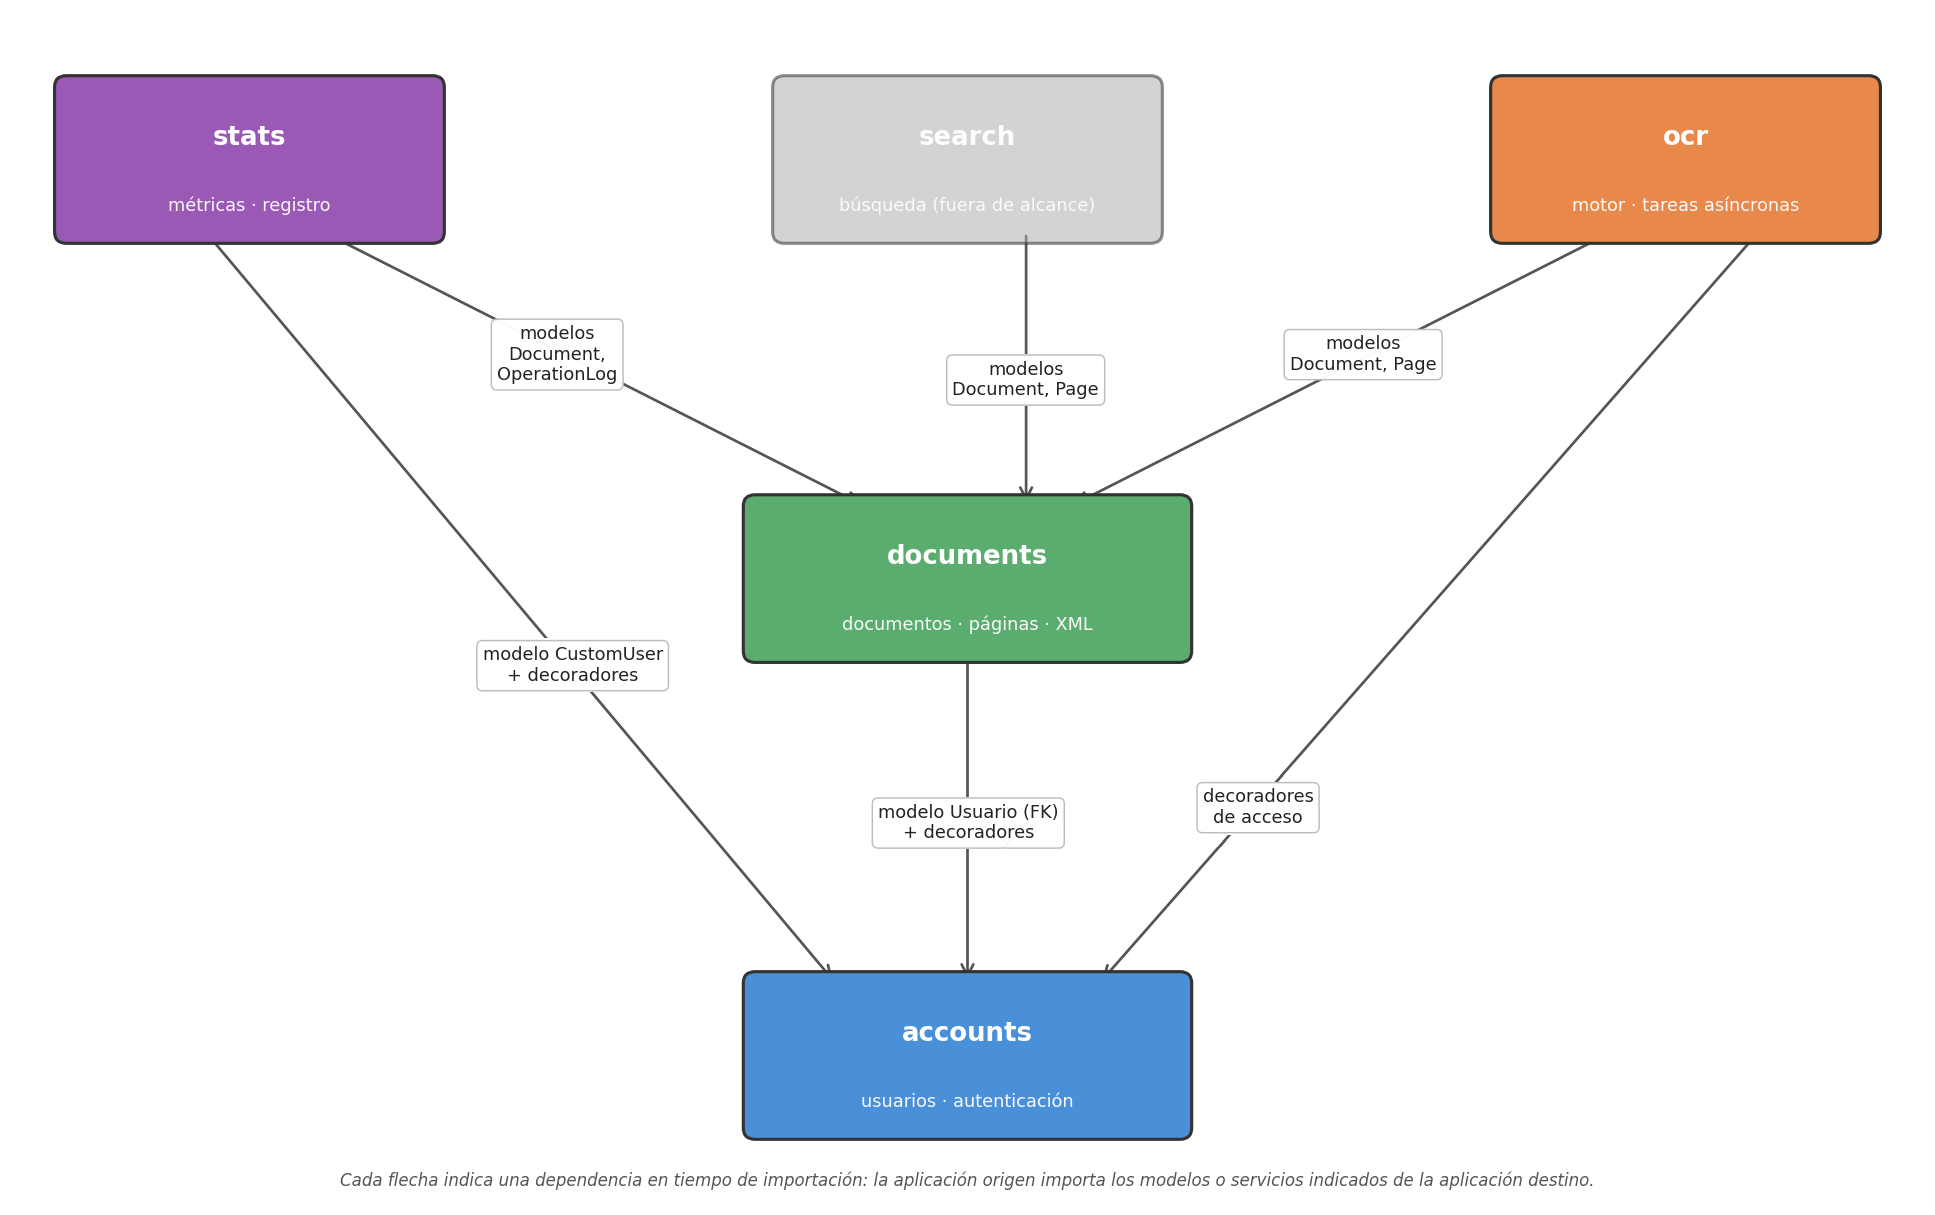
\includegraphics[width=0.88\textwidth]{Graphics/apps_diagram.png}
	\caption{Diagrama de dependencias entre las cinco aplicaciones del proyecto Django. Cada flecha apunta de la aplicación que importa hacia la que provee, y la etiqueta identifica los modelos o servicios concretos que se importan. La aplicación \textit{search} se incluye por completitud pero queda fuera del alcance de esta tesis.}
	\label{fig:apps-diagrama}
\end{figure}

La separación en cinco aplicaciones responde a tres objetivos. El primero es el aislamiento de responsabilidades: cada aplicación encapsula un dominio funcional con sus modelos de datos, vistas y las plantillas que les corresponden, sin acoplamiento innecesario al resto. El segundo objetivo es la facilidad de mantenimiento: cuando una funcionalidad requiere modificación, el desarrollador puede localizar el código sin recorrer el proyecto completo. El tercer objetivo es la reusabilidad: una aplicación bien aislada podría incorporarse a otro proyecto Django con cambios mínimos.

La persistencia adopta una estrategia híbrida. PostgreSQL almacena los datos relacionales que requieren consultas eficientes, transacciones e integridad referencial: usuarios, metadatos de documentos, metadatos de páginas (la ruta al facsímil, el número de orden dentro del documento y el estado del procesamiento OCR), registros de operaciones y métricas de uso. El sistema de ficheros almacena los datos voluminosos que el sistema consulta mayoritariamente por su identificador y rara vez por sus contenidos: imágenes facsimilares y transcripciones en formato XML. La estrategia evita sobrecargar la base de datos con \textit{blobs} binarios y mantiene la facilidad de inspección manual que requiere el flujo de digitalización de documentos.

% -----------------------------------------------------------------------------
\section{Modelo de datos}
\label{sec:modelo-datos}

El modelo de datos relacional comprende cuatro entidades principales que enlazan mediante claves foráneas: el usuario, el documento, la página y el registro de operaciones. La figura~\ref{fig:mer-diagrama} resume el Modelo Entidad-Relación, con los atributos de cada entidad y las relaciones de cardinalidad que las conectan. El esquema completo de la base de datos lo gestiona el sistema de migraciones de Django, que mantiene la coherencia entre los modelos del código fuente y las tablas físicas.

El esquema satisface las condiciones de la forma normal de Boyce-Codd~\cite{codd1972normalization}. La primera forma normal queda satisfecha por construcción: todos los atributos toman valores atómicos, sin estructuras anidadas ni listas dentro de campos individuales. La segunda forma normal queda satisfecha trivialmente porque las claves primarias de las cuatro entidades son simples (el campo \texttt{id} en todos los casos), por lo que no existen dependencias parciales sobre claves compuestas. La tercera forma normal queda satisfecha por inspección directa: ningún atributo no clave de una entidad depende transitivamente de la clave primaria a través de otro atributo no clave. Los atributos \texttt{created\_by\_id} y \texttt{last\_modified\_by\_id} de la entidad documento, por ejemplo, son claves foráneas a la entidad usuario y no derivan ningún otro atributo de la propia entidad documento. La forma normal de Boyce-Codd queda satisfecha porque cada dependencia funcional del esquema tiene como determinante una superclave: la clave primaria \texttt{id} en todas las entidades, o la pareja \texttt{(document\_id, order)} en la entidad página, que el esquema declara como restricción única y que constituye una clave candidata alternativa.

Dos decisiones de diseño del esquema merecen justificación explícita. La primera es la representación del rol del usuario como un atributo de tipo enumerado con tres valores fijos (\textit{trabajador}, \textit{administrador} y \textit{administrador principal}), en lugar de una entidad \textit{Rol} separada con su propia tabla y referencias mediante clave foránea. La elección responde a que los tres roles son categorías institucionales cerradas, sin atributos propios que justifiquen una entidad aparte: el rol carece de descripción extendida, de almacenar datos o metadatos de permisos explícitos que el sistema requiera vincular al rol y que pudieran crecer con el tiempo. La lógica de cada rol vive en el código, no en la base de datos, y se materializa en los decoradores de control de acceso que la sección~\ref{sec:roles-acceso} describe. La decisión simplifica el esquema y elimina una unión adicional en cada consulta sobre usuarios, a cambio de exigir una migración del código y de la base de datos si en el futuro el centro necesita añadir o eliminar roles. La consecuencia es aceptable dado el carácter estable de la estructura institucional del archivo.

La segunda decisión es la ausencia de campos que almacenen las rutas a los ficheros XML de transcripción y a las visualizaciones de segmentación de líneas. La razón es que el identificador del documento y el número de orden de la página determinan unívocamente la ruta de cualquiera de los ficheros. La función \texttt{transcript\_path(document\_id, page\_order)} del módulo de transcripciones construye la ruta de la forma
\begin{quote}
	\centering
	\texttt{\{MEDIA\_ROOT\}/transcripts/\{document\_id\}/page\_\{order:03d\}.xml}
\end{quote}
y una función análoga construye la ruta para visualizar la segmentación que el sistema guarda en caché bajo el subdirectorio \texttt{segmentation/}. La ruta, por tanto, deriva de otros atributos de la página, y almacenarla como campo violaría la tercera forma normal al introducir una dependencia transitiva entre atributos no clave. La aproximación garantiza que cada página tenga su transcripción y su visualización en una ubicación canónica y predecible, sin posibilidad de inconsistencia entre la base de datos y el sistema de ficheros.

\begin{figure}[!htbp]
	\centering
	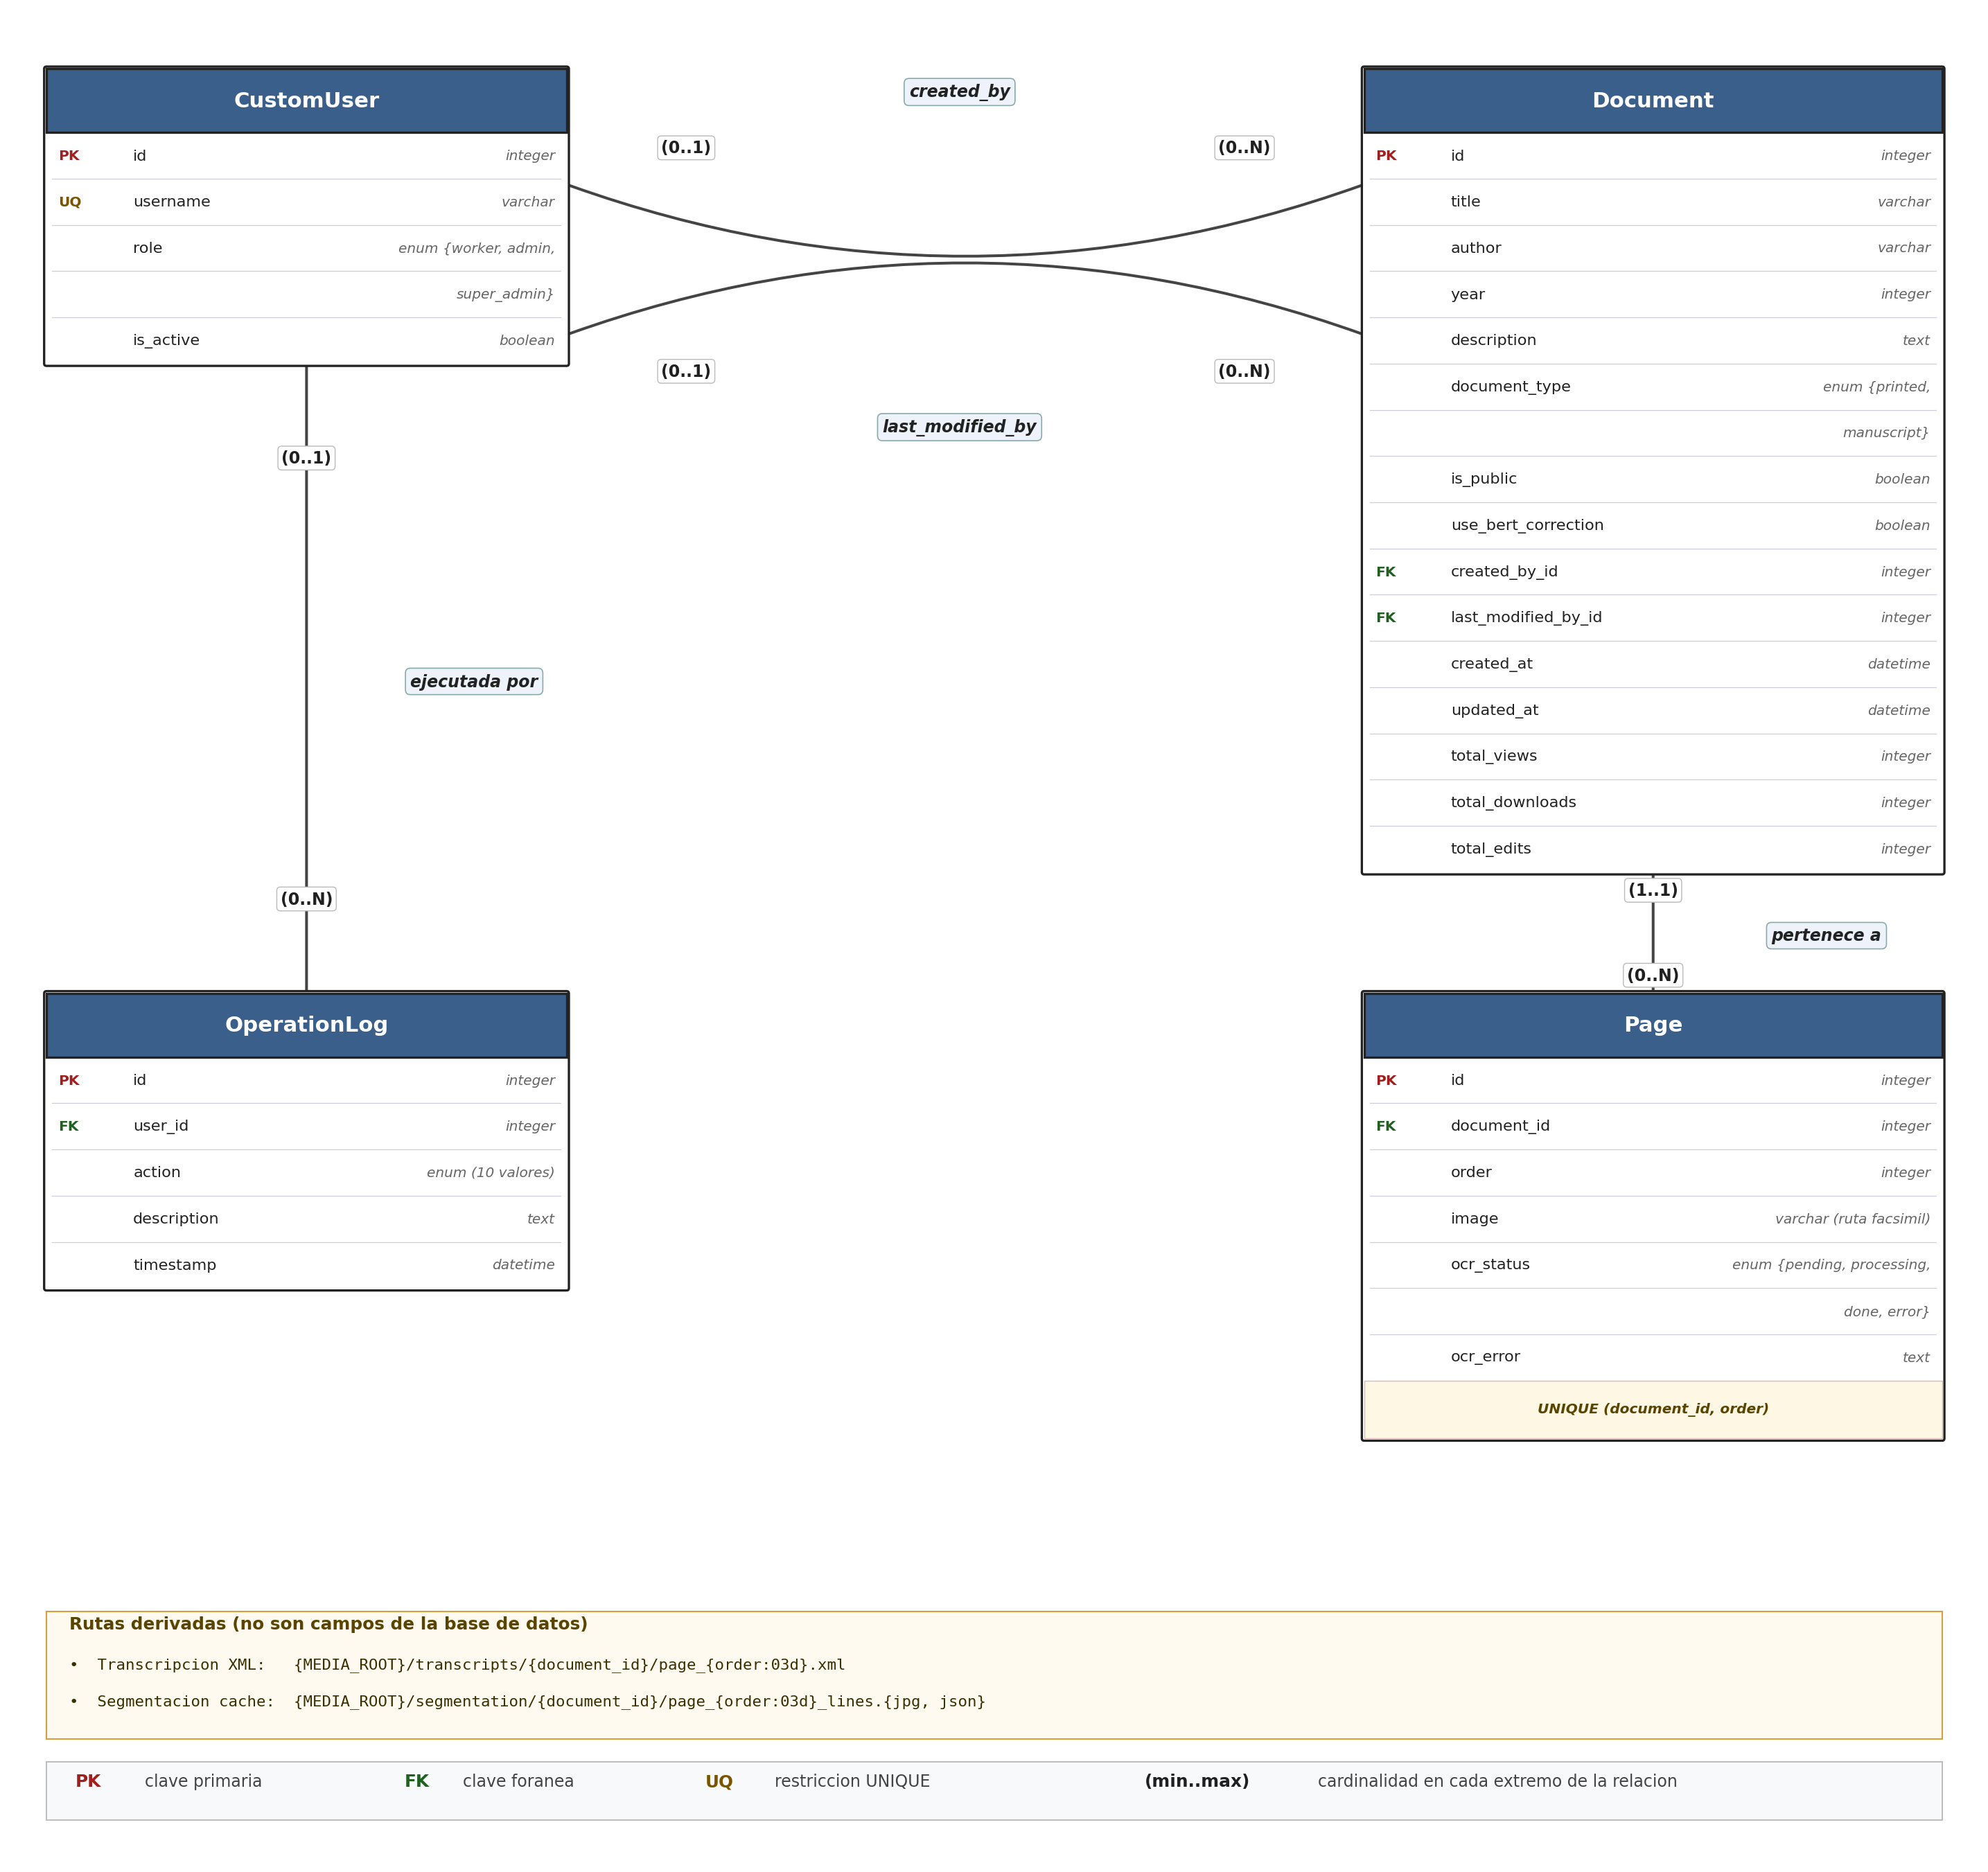
\includegraphics[width=\textwidth]{Graphics/mer_diagram.png}
	\caption{Diagrama Modelo Entidad-Relación del esquema relacional de la aplicación web. Las claves primarias se marcan con \textcolor{red!60!black}{\textbf{PK}}, las claves foráneas con \textcolor{green!40!black}{\textbf{FK}} y las restricciones de unicidad con \textcolor{orange!60!black}{\textbf{UQ}}. Cada línea entre dos entidades representa una relación, con la cardinalidad mínima y máxima entre paréntesis en cada extremo. La nota al pie del diagrama documenta las dos rutas que se derivan del identificador del documento y del orden de la página, sin almacenarse como campos en la base de datos.}
	\label{fig:mer-diagrama}
\end{figure}

\subsection{Documentos y páginas}
\label{subsec:documentos-paginas}

La entidad documento representa una obra digitalizada del archivo del centro Juan Marinello: un libro, una revista, un expediente, una carta u otro tipo de archivo. Cada documento agrupa una o más páginas. Los atributos principales del documento son el título, el año de publicación, el autor, una descripción libre, el tipo del documento, un indicador de visibilidad pública, y referencias al usuario que lo creó y al último que lo modificó. El tipo del documento toma uno de dos valores: \textit{impreso} o \textit{manuscrito}. El presente trabajo cubre únicamente el caso impreso; el caso manuscrito queda fuera del alcance y el capítulo no lo desarrolla.

El indicador de visibilidad pública gobierna el acceso de los usuarios no autenticados. Un documento público es visible para cualquier visitante del sitio sin necesidad de registro, mientras que un documento privado requiere autenticación con un rol que disponga del permiso de lectura. El indicador permite al centro mantener parte del archivo en consulta abierta y reservar el resto a usuarios institucionales.

La entidad página representa un facsímil individual dentro de un documento. Cada página almacena su número de orden dentro del documento, la imagen facsimilar, y el estado del procesamiento OCR. El estado toma uno de cuatro valores: \textit{pendiente}, \textit{en proceso}, \textit{listo} o \textit{error}. La transición entre estados la gestiona el componente que coordina las tareas en \textit{background}, que la sección~\ref{sec:flujo-digitalizacion} describe.

El texto que el OCR produce, junto con las regiones que el usuario pueda definir sobre la página, no descansa en la base de datos relacional sino en un fichero XML por página. La sección~\ref{sec:formato-xml} desarrolla la decisión y el formato del fichero. El acceso al texto desde el código opera mediante los métodos \texttt{get\_text} y \texttt{set\_text} que la página expone, los cuales delegan en una capa específica que encapsula toda la entrada y salida de ficheros XML. El resto del proyecto interactúa siempre a través de la página, sin tocar el sistema de ficheros directamente.

Una segunda categoría de ficheros que el sistema vincula a cada página son las visualizaciones de la segmentación de líneas, que el editor de revisión emplea para superponer las cajas de líneas sobre el facsímil. El sistema calcula la visualización la primera vez que el editor la solicita, junto con un fichero JSON que contiene las coordenadas exactas de las cajas, y guarda ambos en el subdirectorio \texttt{segmentation/} de la ruta del documento. La estrategia evita recalcular la segmentación en cada apertura del editor.

\subsection{Registro de operaciones y métricas de uso}
\label{subsec:auditoria}

El sistema mantiene un registro de auditoría con todas las operaciones que modifican el estado del archivo: inserción, edición o eliminación de documentos, inserción o eliminación de usuarios, cambios de privilegios, y eventos de inicio y cierre de sesión. Cada entrada del registro guarda el usuario que ejecutó la acción, el tipo de acción según un catálogo cerrado, una descripción textual del cambio, y la marca de tiempo. El registro permite reconstruir la historia de cualquier documento ante una incidencia y atribuir responsabilidades cuando varios usuarios colaboran sobre el mismo material.

Las métricas de uso complementan al registro de auditoría con tres contadores incrementales por documento: el número total de visualizaciones, el número total de descargas y el número total de ediciones. Los tres contadores los actualiza el código en las vistas correspondientes mediante operaciones atómicas que evitan condiciones de carrera entre peticiones simultáneas. Las métricas alimentan los paneles de la aplicación \textit{stats} y orientan al equipo del centro sobre los materiales con mayor número de consultas.

El sistema garantiza la coherencia entre la base de datos relacional y los ficheros del sistema durante las operaciones de borrado mediante \textit{signals} de Django que conectan al evento \textit{post-delete}. Cuando la base de datos elimina una página, un manejador borra el fichero del facsímil, el fichero XML de transcripción y los ficheros de la visualización de segmentación que la caché guarda. Cuando la base elimina un documento, el borrado en cascada del modelo relacional propaga la eliminación a todas sus páginas, y un segundo manejador limpia los directorios del documento en los tres subdirectorios \texttt{facsimiles/}, \texttt{transcripts/} y \texttt{segmentation/} por si hubiera quedado algún fichero huérfano de procesos anteriores. El mecanismo evita la acumulación de ficheros sin referencia en disco a medida que el archivo crece o las operaciones de reorganización avanzan.

% -----------------------------------------------------------------------------
\section{Roles de usuario y control de acceso}
\label{sec:roles-acceso}

El sistema distingue tres roles para los usuarios autenticados: trabajador, administrador y administrador principal. Cada rol amplía las capacidades del anterior. La tabla~\ref{tab:roles} resume las capacidades concretas de cada rol.

\begin{table}[!htbp]
	\centering
	\caption{Capacidades que el sistema concede a cada rol.}
	\label{tab:roles}
	\begin{tabular}{lp{10cm}}
		\toprule
		\textbf{Rol} & \textbf{Capacidades} \\
		\midrule
		Trabajador & Sube documentos nuevos, ejecuta OCR sobre las páginas, edita y corrige las transcripciones que el modelo produce, elimina documentos del archivo y descarga el contenido del archivo. \\
		\addlinespace
		Administrador & Las del trabajador y, adicionalmente, gestiona los usuarios con rol de trabajador, accede al registro de operaciones y a las métricas de uso. \\
		\addlinespace
		Administrador principal & Las del administrador y, adicionalmente, crea o elimina otros administradores. La instalación inicial del sistema crea un administrador principal mediante un comando específico de la línea de órdenes de Django. \\
		\bottomrule
	\end{tabular}
\end{table}

El sistema aplica el control de acceso mediante decoradores que envuelven las vistas. Cada vista declara el rol mínimo que requiere para ejecutarse. Cuando un usuario sin el rol suficiente intenta acceder, el decorador devuelve una respuesta de denegación con el código de estado apropiado, sin que el código de la vista llegue a ejecutarse. La estrategia centraliza la lógica de autorización y evita la dispersión de comprobaciones a lo largo del proyecto.

Los visitantes que no se autentican pueden consultar y descargar los documentos públicos, así como buscar dentro de su contenido. La distinción permite al centro publicar parte del archivo sin obligar a los lectores ocasionales a registrarse, mientras se reserva el material no público a los usuarios con rol institucional.

% -----------------------------------------------------------------------------
\section{Flujo de digitalización}
\label{sec:flujo-digitalizacion}

El flujo completo que recorre un documento desde su entrada al sistema hasta su consulta final comprende cinco fases: subida, procesamiento OCR asíncrono, revisión manual, almacenamiento y consulta. La figura~\ref{fig:flujo-digitalizacion} resume las cinco fases en secuencia; los párrafos siguientes las desarrollan en detalle.

\begin{figure}[!htbp]
	\centering
	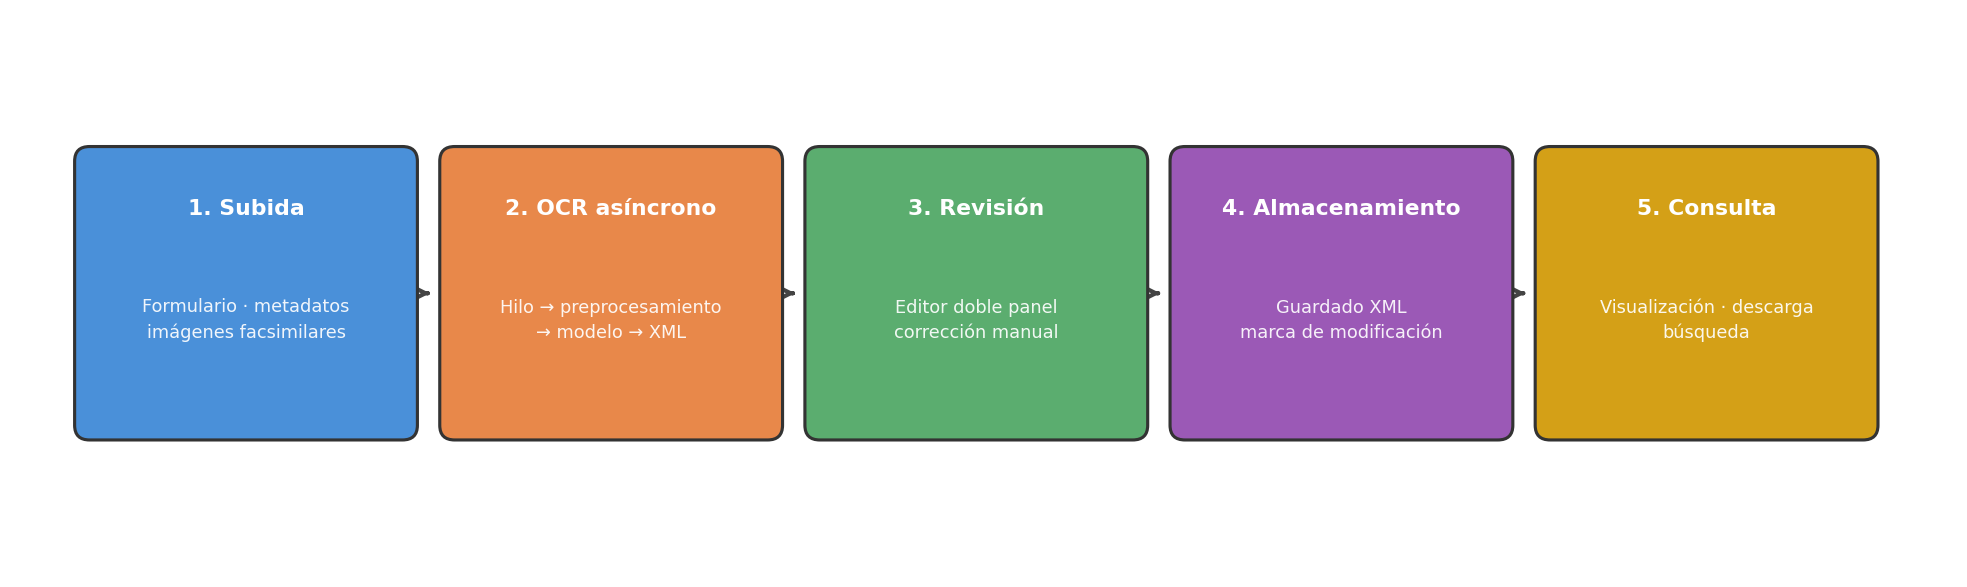
\includegraphics[width=\textwidth]{Graphics/flujo_digitalizacion.png}
	\caption{Las cinco fases del flujo de digitalización: subida, procesamiento OCR asíncrono, revisión manual, almacenamiento y consulta.}
	\label{fig:flujo-digitalizacion}
\end{figure}

La fase de subida la inicia el usuario al crear un documento nuevo mediante el formulario de inserción. El usuario aporta los metadatos del documento y selecciona las imágenes facsimilares correspondientes a las páginas. El \textit{framework} valida los formularios mediante el sistema declarativo de validación de Django, persiste los metadatos del documento y de las páginas en la base de datos, y guarda cada imagen en el sistema de ficheros bajo una ruta determinista que organiza los facsímiles por documento. Las páginas que la subida crea quedan inicialmente en estado pendiente, sin transcripción.

La fase de procesamiento OCR la inicia el sistema inmediatamente después de la subida, sin intervención del usuario. La invocación del OCR sobre todas las páginas de un documento de cien páginas, ejecutada de forma sincrónica dentro de la petición HTTP~\cite{ietf2022http}, tardaría varios minutos y desbordaría los tiempos de respuesta habituales. La aplicación adopta en su lugar un esquema asíncrono basado en hilos. Cuando el usuario completa la subida, la vista correspondiente arranca un hilo propio del documento, devuelve la respuesta HTTP inmediatamente y libera al usuario para que continúe trabajando o consulte el progreso. El hilo recorre las páginas pendientes por orden, marca cada una como en proceso, ejecuta el OCR, almacena la transcripción y deja la página en estado listo, o en estado error si el procesamiento falla. La interfaz consulta periódicamente el estado del documento y desbloquea cada página a medida que el hilo la completa.

El esquema basado en hilos presenta una limitación frente a una cola de tareas externa con persistencia propia y \textit{workers} independientes del proceso del servidor web: si el proceso de Django muere a mitad del procesamiento, las páginas que estaban en proceso quedan huérfanas con su estado intermedio. El sistema mitiga la limitación mediante una rutina de recuperación que arranca con el servidor: la rutina detecta las páginas que llevan más de un umbral de tiempo en estado de procesamiento, las marca de vuelta como pendientes, y desencadena un nuevo intento sobre los documentos afectados. El esquema sin cola externa resulta adecuado para volúmenes moderados de subidas simultáneas como los que el contexto del centro Juan Marinello espera; un crecimiento sustancial de la demanda justificaría la migración a una infraestructura con cola persistente y \textit{workers} específicos del procesamiento OCR.

La aplicación admite además la cancelación del procesamiento cuando el usuario decide abandonar un documento durante la subida. La vista de abandono inserta el identificador del documento en un conjunto de cancelaciones pendientes que el hilo del OCR consulta entre página y página: cuando el identificador aparece en el conjunto, el hilo termina de procesar la página actual y sale del bucle sin tocar las páginas pendientes. El procesamiento de la página en curso no admite interrupción a la fuerza porque el modelo de PyTorch no soporta interrupción limpia a mitad de inferencia. Una vez cancelado, el documento admite eliminación mediante la vista correspondiente, que el sistema concede a cualquier usuario con rol de trabajador o superior.

Además del procesamiento automático al subir el documento, la aplicación ofrece dos botones en el editor que permiten al usuario lanzar el OCR sobre alcances más estrechos. El primero, identificado como \emph{Re-ejecutar OCR}, reprocesa la página que el usuario tiene abierta; el sistema la marca de vuelta como pendiente, ejecuta el \textit{pipeline} completo y actualiza la transcripción cuando termina. El segundo, identificado como \emph{OCR de regiones}, restringe el reconocimiento a las cajas que el usuario haya dibujado sobre el facsímil y sustituye la transcripción de la página con el texto que produce cada región en el orden que el usuario asignó. Ambos botones comparten el mismo motor OCR y la misma capa de persistencia que el procesamiento inicial. La figura~\ref{fig:editor-botones} ilustra su posición en la interfaz del editor.

\begin{figure}[!htbp]
	\centering
	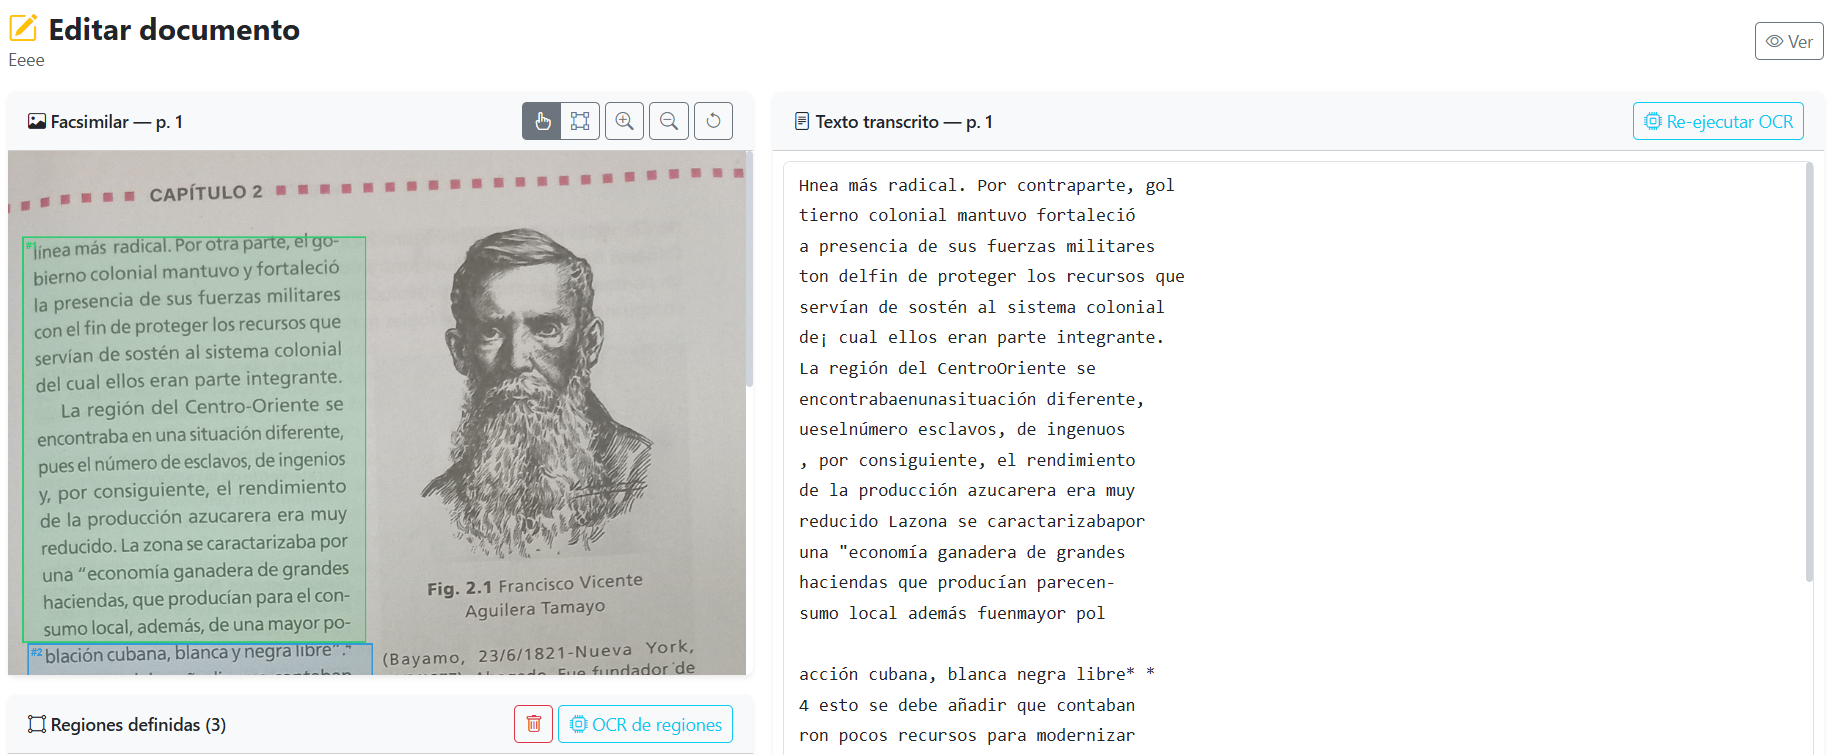
\includegraphics[width=0.92\textwidth]{Graphics/editor_botones.png}
	\caption{Botones de reconocimiento del editor: \emph{Re-ejecutar OCR} (panel derecho, esquina superior) para reprocesar la página completa, y \emph{OCR de regiones} (panel izquierdo, sección de regiones) para restringir el reconocimiento a las cajas que el usuario haya definido.}
	\label{fig:editor-botones}
\end{figure}

La fase de revisión manual la inicia el usuario al abrir la página de edición de cualquier página que ya esté en estado listo. La interfaz presenta al usuario el facsímil junto a la transcripción que el modelo produjo en un diseño de doble panel, y permite corregir los errores de reconocimiento. La figura~\ref{fig:editor-facsimil} muestra el aspecto del editor una vez que el OCR ha completado la página. Las características detalladas del editor se desarrollan en la sección~\ref{sec:editor}.

\begin{figure}[!htbp]
	\centering
	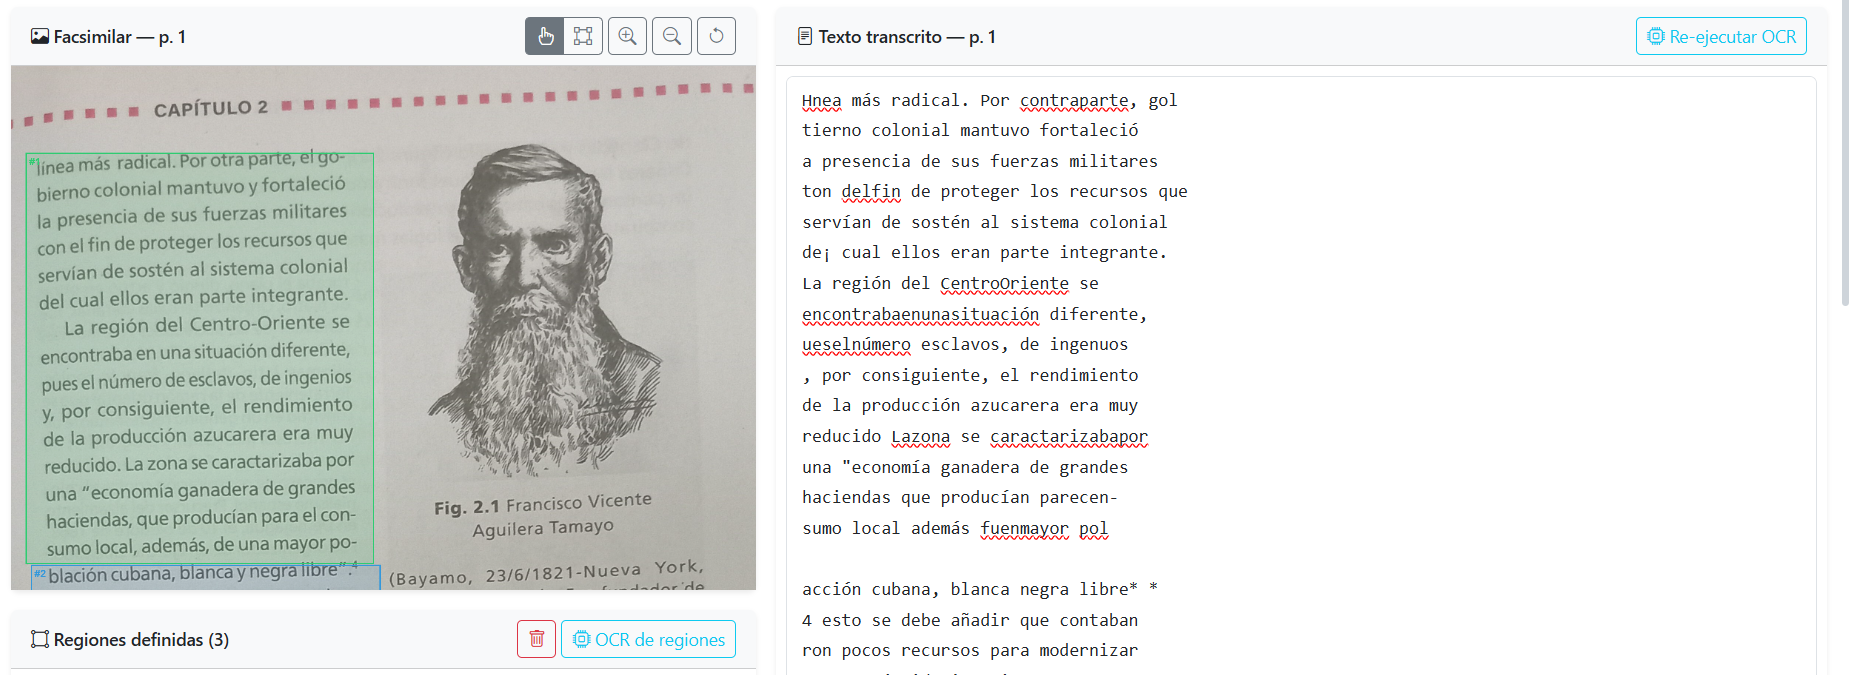
\includegraphics[width=0.9\textwidth]{Graphics/editor_facsimil_transcripcion.png}
	\caption{Editor de revisión con diseño de doble panel: el facsímil de la página en el panel izquierdo y la transcripción que el modelo produjo en el panel derecho, disponible para edición.}
	\label{fig:editor-facsimil}
\end{figure}

La fase de almacenamiento opera al guardar las correcciones del usuario. El sistema persiste las correcciones del usuario en el fichero XML correspondiente a la página, mediante la capa de transcripciones que la subsección~\ref{subsec:documentos-paginas} mencionó. La capa preserva los metadatos del documento y la marca de creación original del fichero, y actualiza la marca de última modificación.

La fase de consulta agrupa las acciones de lectura sobre el archivo ya digitalizado: visualización del documento por sus páginas, descarga del facsímil o de la transcripción, y búsqueda por título o contenido. Cada visualización incrementa el contador de visualizaciones del documento, cada descarga incrementa el contador de descargas, y cada edición incrementa el contador de ediciones, según describió la subsección~\ref{subsec:auditoria}.

% -----------------------------------------------------------------------------
\section{Integración del modelo de reconocimiento}
\label{sec:integracion-ocr}

La integración del modelo de reconocimiento que el capítulo~\ref{chap:modelo} desarrolla con la aplicación web requiere tres puntos de articulación: la carga del modelo en memoria, la invocación del \textit{pipeline} de preprocesamiento, y la composición del texto reconocido para su almacenamiento.

La carga del modelo en memoria opera al arranque del proceso Django, no en respuesta a la primera petición. La estrategia evita que el primer usuario que invoca el OCR sufra una latencia inicial de varios segundos por la lectura de los pesos del modelo. Cuando el servidor Django arranca, un hilo en \textit{background} ejecuta una rutina de precarga que invoca los cinco modelos del sistema en un orden fijo: el modelo de lenguaje de \textit{n}-gramas a nivel de carácter, que el equipo entrenó previamente sobre \textit{corpus} de español de uso general y que la herramienta KenLM~\cite{heafield2011kenlm} carga; el corrector ortográfico SymSpell~\cite{garbe2012symspell}; el modelo CRNN+CTC~\cite{shi2016crnn,graves2006ctc} para impresos que el capítulo~\ref{chap:modelo} desarrolla; el modelo HTR para manuscritos --que queda fuera del alcance de esta tesis-- y el \textit{reranker} neuronal sobre BETO~\cite{canete2020beto}. La precarga ocurre en \textit{background} para no bloquear el arranque del servidor, y los cinco modelos quedan como singletons disponibles para las peticiones que llegan después. Cada singleton incorpora un mecanismo de bloqueo con doble verificación que protege contra cargas concurrentes en el caso de que una petición OCR llegue antes de que la precarga termine: la petición simplemente espera al bloqueo sin iniciar una segunda carga del mismo modelo. La inicialización lee los pesos que el entrenamiento del capítulo~\ref{chap:modelo} produjo y los carga en el dispositivo de cómputo que la instalación configura, que es la CPU por defecto pero puede ser una GPU si la instalación dispone de ella.

La invocación del \textit{pipeline} de preprocesamiento sobre cada página sigue las cinco etapas que el capítulo~\ref{chap:preprocesamiento} describió: análisis y configuración automática, binarización, corrección de inclinación a tres niveles, detección y segmentación de bloques y líneas, y normalización de cada línea para inferencia. La salida del \textit{pipeline} es una lista ordenada de líneas con altura uniforme de sesenta y cuatro píxeles y anchos variables, en el formato exacto que el modelo del capítulo~\ref{chap:modelo} espera como entrada.

La inferencia del modelo opera sobre las líneas en lotes para amortizar el coste fijo de cada llamada al dispositivo de cómputo. Cada lote agrupa líneas de anchos similares para reducir el desperdicio de relleno, según una estrategia análoga a la del muestreador por agrupamiento que la subsección~
ef{subsec:bucketing} describió. La decodificación adopta la búsqueda en haz con el modelo de lenguaje de cinco gramas que la subsección~\ref{subsec:lm-posterior} describe, configuración que mejora el rendimiento sobre documentos reales gracias a la mayor incertidumbre acústica del modelo visual ante degradaciones de escaneado y a la regularidad morfológica del español.

La composición del texto para su almacenamiento concatena las transcripciones de las líneas individuales con saltos de línea, preservando el orden vertical que el \textit{pipeline} estableció durante la segmentación. La concatenación pasa por la capa de transcripciones, que escribe el fichero XML correspondiente con el texto, los metadatos del documento y la marca de tiempo de creación.

La aplicación admite además una variante del procesamiento que opera sobre regiones definidas por el usuario en lugar de sobre la página completa. La variante resulta útil cuando el usuario quiere transcribir solamente una porción del facsímil, como un párrafo de interés dentro de un documento extenso o un fragmento legible dentro de una página parcialmente dañada. El usuario marca las regiones en el editor mediante el ratón, el sistema las guarda en el XML como cajas con coordenadas en píxeles del facsímil original, y el motor de OCR recorta cada caja antes de procesarla con el mismo \textit{pipeline} de preprocesamiento. La salida produce un texto que respeta el orden que el usuario asignó a las regiones.

El procesamiento de cada página por el motor OCR aplica un postprocesado al texto que la decodificación con búsqueda en haz y modelo de lenguaje produce, antes de almacenarlo. El postprocesado consta de un paso obligatorio y un paso opcional. El paso obligatorio es la corrección ortográfica mediante SymSpell~\cite{garbe2012symspell}, un corrector basado en distancia de edición y diccionario de frecuencias del español. SymSpell propone candidatos para cada palabra que no aparece en el diccionario y los ordena por una combinación de proximidad ortográfica y frecuencia en el idioma. El paso opcional es el \textit{reranking} neural: las palabras con varios candidatos plausibles se desambiguan mediante un modelo de lenguaje contextual basado en BETO que evalúa cada candidato en el contexto de la oración completa. La opción mejora la calidad en casos ambiguos a costa de una latencia adicional por página.

% -----------------------------------------------------------------------------
\section{Editor de revisión de transcripciones}
\label{sec:editor}

El reconocimiento automático rara vez produce una transcripción perfecta. Los errores residuales típicos incluyen confusiones entre signos de puntuación visualmente similares y omisión de tildes en cuerpos tipográficos pequeños, según se identificó en la sección~\ref{sec:fine-tuning} del capítulo anterior, junto con errores en regiones con tinta desvanecida o sangrado severo cuando la calidad del facsímil cae fuera del rango que el preprocesamiento puede compensar. La aplicación incorpora un editor de revisión que permite al usuario corregir los errores residuales con la imagen original visible como referencia.

El editor adopta un diseño de doble panel. El panel izquierdo muestra el facsímil de la página a tamaño completo, con la posibilidad de hacer zoom y desplazamiento mediante el ratón y el teclado. El panel derecho contiene un área de texto editable con la transcripción que el modelo produjo. El usuario lee la transcripción mientras consulta el facsímil para verificar las dudas, modifica los caracteres incorrectos en el área de texto, y guarda los cambios cuando termina la revisión de la página. La interfaz no impone separación rígida entre líneas: el área de texto presenta la transcripción como un cuerpo continuo que el usuario edita como cualquier texto plano. La figura~\ref{fig:editor-completo} muestra el editor con ambos paneles activos.

\begin{figure}[!htbp]
	\centering
	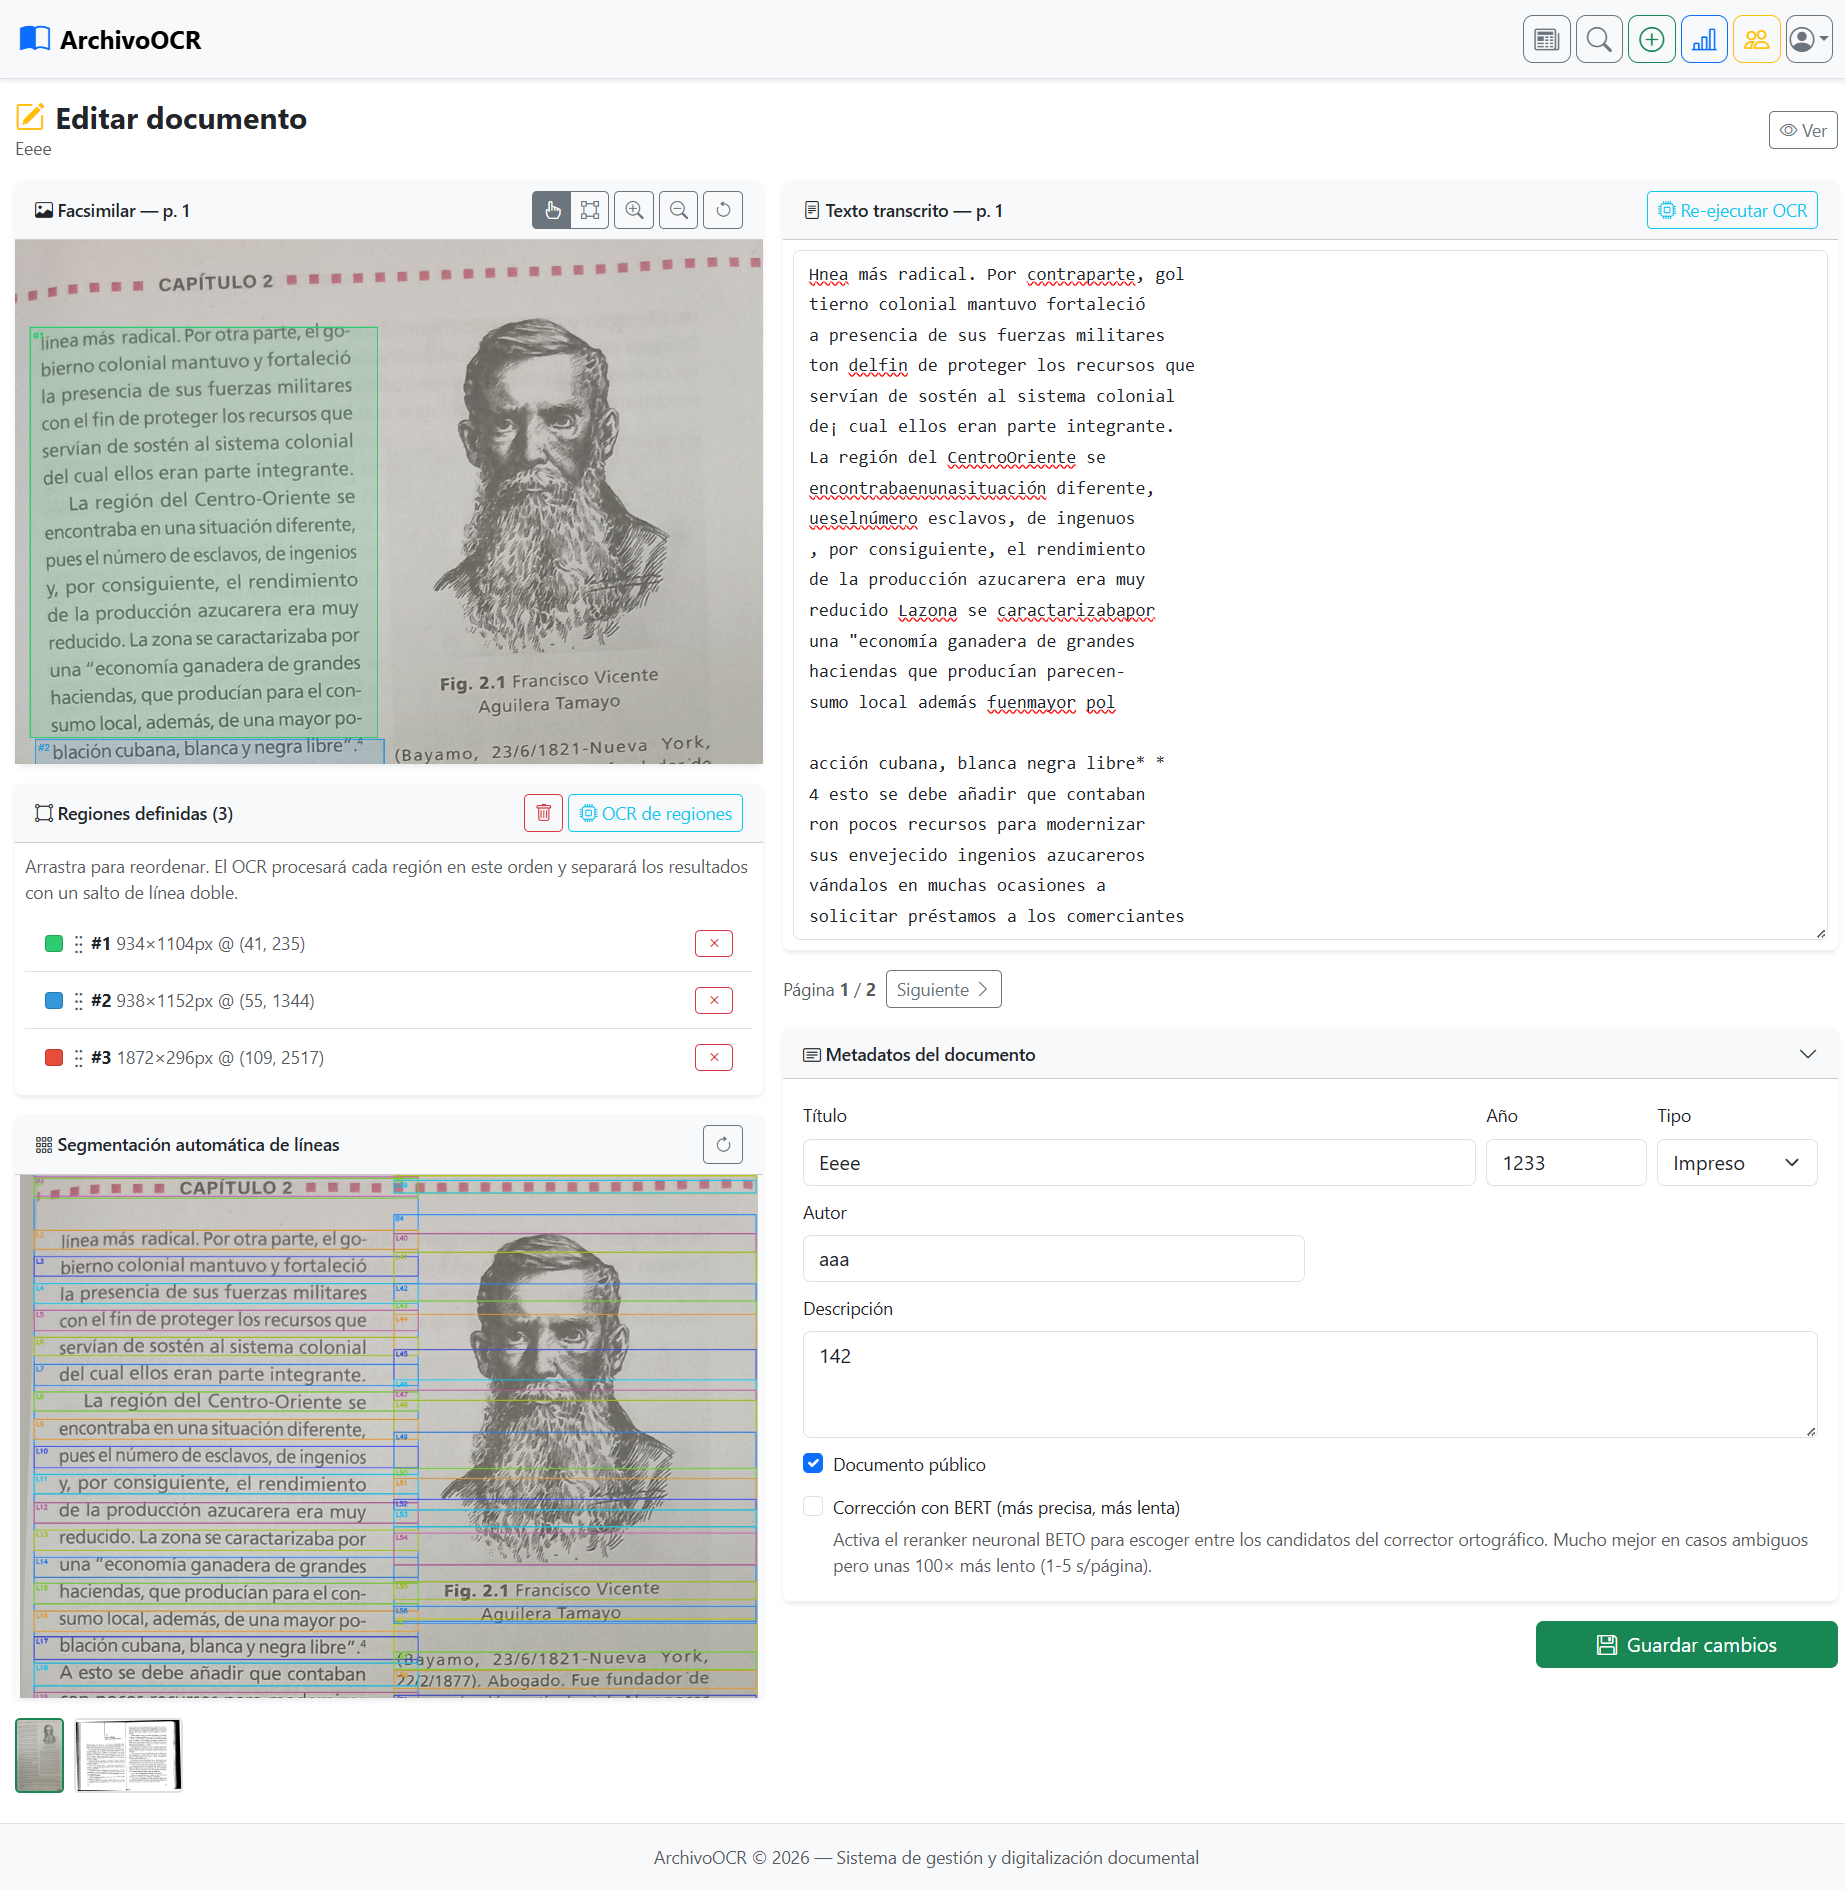
\includegraphics[width=0.78\textwidth]{Graphics/editor_completo.png}
	\caption{Vista completa del editor de revisión con el facsímil de la página arriba y la visualización de segmentación de líneas abajo en el panel izquierdo, y el texto que el modelo produjo en el panel derecho, junto al aviso de guardado.}
	\label{fig:editor-completo}
\end{figure}

Una segunda funcionalidad del editor permite visualizar la segmentación de líneas que el \textit{pipeline} de preprocesamiento produjo sobre la página. La visualización superpone, sobre el facsímil del panel izquierdo, las cajas que delimitan cada línea según la detección del capítulo~\ref{chap:preprocesamiento}. La superposición resulta útil para diagnosticar problemas de segmentación: una línea que el sistema no detectó, dos líneas que se unieron en una sola, o una caja desplazada respecto al texto. El usuario puede entonces volver al material físico, escanear la página en mejores condiciones, o aceptar el resultado tras valorar la magnitud del error. La figura~\ref{fig:editor-segmentacion} muestra la visualización de segmentación superpuesta sobre el facsímil.

\begin{figure}[!htbp]
	\centering
	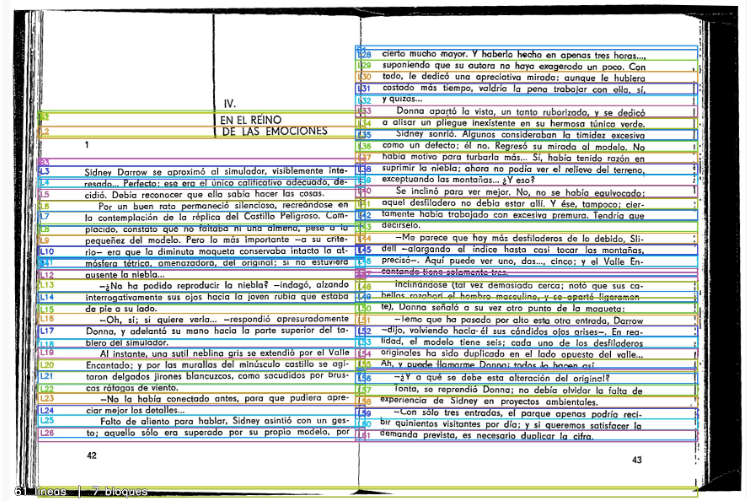
\includegraphics[width=0.6\textwidth]{Graphics/editor_segmentacion.png}
	\caption{Panel izquierdo del editor con la visualización de segmentación activa. Cada caja de color delimita una línea que el \textit{pipeline} del capítulo~\ref{chap:preprocesamiento} detectó; las etiquetas L1, L2,~\ldots{} identifican el orden de lectura.}
	\label{fig:editor-segmentacion}
\end{figure}

El editor incorpora una protección contra escrituras concurrentes cuando el OCR aún está en curso sobre el documento. Mientras alguna página del documento permanece en estado pendiente, en proceso o de error, el editor permite al usuario navegar entre páginas pero rechaza cualquier intento de guardar cambios sobre el texto. La protección evita que el hilo del OCR, al terminar de procesar una página, sobrescriba con su transcripción el texto que el usuario hubiera comenzado a editar manualmente en la misma página. Una vez que todas las páginas alcanzan el estado de listas, el editor desbloquea el guardado y el usuario puede corregir libremente las transcripciones.

La definición de regiones por el usuario, que el final de la sección anterior mencionó, también opera en el editor. El usuario arrastra el ratón sobre el facsímil para dibujar cajas, asigna el orden con que quiere que el sistema las procese, y desencadena el reconocimiento, que el sistema restringe a las regiones que el usuario dibujó. El resultado sustituye, en el área de texto, a la transcripción anterior de la página.

Más allá de la edición de la transcripción, el editor ofrece tres operaciones complementarias sobre el documento. La primera es el abandono de la edición, que descarta los cambios que el usuario todavía no ha guardado. La segunda es la eliminación del documento, disponible para cualquier usuario con rol de trabajador o superior, según se detalló en la sección~\ref{sec:roles-acceso}. La tercera es la descarga del documento, que produce un documento PDF~\cite{iso2020pdf} o EPUB~\cite{w3c2023epub} con la transcripción completa del archivo, con la opción adicional de incluir los facsímiles originales junto al texto.

% -----------------------------------------------------------------------------
\section{Formato XML y exportación a estándares}
\label{sec:formato-xml}

La transcripción de cada página se almacena en un fichero XML independiente, según se introdujo en la subsección~\ref{subsec:documentos-paginas}. La presente sección desarrolla la estructura del fichero y las decisiones de diseño que la sustentan.

\subsection{Estructura del fichero}
\label{subsec:estructura-xml}

El fichero XML de una página contiene cinco bloques principales: un identificador del documento al que pertenece, los metadatos básicos como título, autor, año y tipo, una referencia al facsímil de la página, las marcas de tiempo de creación y última modificación, y el cuerpo de la transcripción organizado en líneas. Un bloque opcional adicional almacena las regiones que el usuario haya definido sobre la página. El esquema completo se ilustra en el siguiente fragmento:

\begin{lstlisting}[language=XML,caption={Estructura del fichero XML de transcripción por página.},label={lst:xml}]
	<?xml version="1.0" encoding="UTF-8"?>
	<Transcript version="1">
	<Document id="42">
	<Title>Don Quijote de la Mancha</Title>
	<Author>Miguel de Cervantes</Author>
	<Year>1605</Year>
	<Type>printed</Type>
	</Document>
	<Page order="3" facsimile="page_003.jpg"/>
	<Timestamps>
	<Created>2026-05-09T14:30:00+02:00</Created>
	<Modified>2026-05-09T14:35:12+02:00</Modified>
	</Timestamps>
	<Regions>
	<Region id="r1" order="1" x="120" y="80" width="900" height="220"/>
	</Regions>
	<Body>
	<Line>En un lugar de la Mancha, de cuyo nombre no quiero acordarme,</Line>
	<Line>no ha mucho tiempo que vivia un hidalgo de los de lanza en astillero,</Line>
	<Line/>
	<Line>adarga antigua, rocin flaco y galgo corredor.</Line>
	</Body>
	</Transcript>
\end{lstlisting}

Cada \texttt{Line} representa un salto lógico de línea. Las líneas vacías que el OCR detecta como separación entre párrafos permanecen como elementos \texttt{Line} sin contenido. La representación en texto plano resulta de concatenar el contenido de los elementos \texttt{Line} con saltos de línea.

\subsection{Decisiones de diseño}
\label{subsec:decisiones-xml}

El esquema responde a tres objetivos. El primer objetivo es la legibilidad humana directa. Un revisor puede abrir cualquier fichero con un editor de texto y entender el contenido sin herramientas auxiliares, lo que reduce la barrera para auditar o reparar manualmente las transcripciones cuando aparece una incidencia. El segundo objetivo es la independencia de bibliotecas externas. La serialización emplea \texttt{ElementTree}, la biblioteca XML que viene con la distribución estándar de Python, sin requerir paquetes adicionales como \texttt{lxml}. El tercer objetivo es la convertibilidad a estándares mayores en caso de que el archivo crezca y requiera interoperabilidad institucional.

La decisión de mantener las transcripciones en ficheros XML y no en filas de la base de datos relacional merece justificación. Los argumentos a favor del XML son tres. Primero, el contenido de una transcripción se consulta casi siempre por su clave de página, no por sus contenidos internos; la base de datos relacional ofrece poca ventaja sobre el sistema de ficheros cuando el patrón de acceso es siempre por clave única. Segundo, el XML resulta inmediatamente exportable, lo que facilita las copias de seguridad y la migración a otro almacenamiento. Tercero, la versión textual de la transcripción puede crecer sin afectar el tamaño de las tablas relacionales, lo que mantiene la base de datos compacta y eficiente para las consultas que sí requieren índices.

Una ventaja adicional del esquema propio es que el conjunto de información que captura constituye un subconjunto de los estándares ALTO~\cite{loc-alto}, PAGE-XML~\cite{pletschacher2010page} y TEI~\cite{tei-consortium}, que los archivos digitales emplean ampliamente. La elección preserva la posibilidad de que el archivo del centro Juan Marinello migre a cualquiera de los tres estándares cuando el sistema se integre en un repositorio institucional con requisitos de interoperabilidad, sin pérdida de información respecto al estado actual.

% -----------------------------------------------------------------------------
% Cierre del capítulo
% -----------------------------------------------------------------------------

La aplicación web que el capítulo describe completa el sistema con la capa de interacción con el usuario. El conjunto del trabajo, desde la generación del \textit{corpus} sintético del capítulo~\ref{chap:corpus} hasta la integración en la aplicación que el capítulo~\ref{chap:web} desarrolla, configura una herramienta operativa para la digitalización del archivo del centro Juan Marinello. Las contribuciones del trabajo, las limitaciones que se identificaron y las líneas de trabajo que quedan abiertas se sintetizan en las conclusiones que cierran el documento.

	
	\backmatter
	\chapter*{Conclusiones}
\addcontentsline{toc}{chapter}{Conclusiones}\label{chap:conclusions}

El trabajo abordó el desarrollo de un sistema OCR para texto impreso en español y su integración en una aplicación web de digitalización documental, en respuesta a la necesidad del Instituto Cubano de Investigación Cultural Juan Marinello de procesar el acervo documental que la institución conserva sobre soporte físico. La solución articula cuatro componentes técnicos —generador de \textit{corpus} sintético, \textit{pipeline} de preprocesamiento, modelo de reconocimiento de secuencias y aplicación web— cuyos resultados resume el listado siguiente.

\begin{enumerate}[leftmargin=*,labelsep=0.5em]
	\item \textbf{Análisis del estado del arte y decisiones de diseño.} El estudio comparativo entre motores OCR clásicos, arquitecturas que operan sobre aprendizaje profundo y plataformas de digitalización documental estableció que la combinación de una red neuronal convolucional recurrente con la función de pérdida CTC ofrece el equilibrio adecuado entre coste de entrenamiento y capacidad de modelado del contexto léxico para el reconocimiento de líneas de texto impreso. La revisión de los conjuntos de datos públicos para OCR en español identificó cuatro limitaciones que descartaban su uso como base de entrenamiento —cobertura incompleta de los caracteres específicos del español, redundancia tipográfica, inviabilidad de corrección por augmentación posterior y ausencia de contexto léxico—, y justificó la generación de un \textit{corpus} sintético propio.
	
	\item \textbf{Corpus sintético.} El trabajo diseñó e implementó un generador de pares imagen--transcripción con control explícito sobre la distribución de frecuencias de caracteres mediante una estrategia de sobremuestreo en tres grupos. El generador toma el texto de obras literarias en español del dominio público disponibles en Project Gutenberg, lo renderiza con un repertorio de quince fuentes tipográficas que cubren tres familias estilísticas (monoespacio, serif clásica y máquina de escribir), y aplica una simulación de degradación visual compatible con los dos métodos de binarización del \textit{pipeline}. El \textit{corpus} final reúne 19\,995 imágenes con cobertura total del vocabulario de cien símbolos, y mantiene todos los caracteres específicos del español formal —vocales con tilde, eñe, comillas angulares, raya de diálogo y signos de apertura de interrogación y exclamación— por encima del umbral mínimo de quinientas apariciones.
	
	\item \textbf{Pipeline de preprocesamiento.} El trabajo implementó un \textit{pipeline} con configuración automática a partir de cinco métricas de imagen, sin intervención del usuario. El \textit{pipeline} elige entre la binarización global de Otsu y la binarización adaptativa de Sauvola según la uniformidad del fondo, corrige la inclinación en tres niveles (global de la página, residual por bloque y curvatura por línea), detecta bloques de texto mediante una variante recursiva del algoritmo XY-Cut robusta a páginas con doble columna y a pliegos abiertos, y segmenta las líneas mediante proyección horizontal de la imagen binaria. La salida del \textit{pipeline} son líneas con altura fija de sesenta y cuatro píxeles, en el formato que el modelo de reconocimiento exige.
	
	\item \textbf{Modelo de reconocimiento y protocolo de evaluación.} El trabajo diseñó, entrenó y evaluó un modelo CRNN con red recurrente bidireccional y función de pérdida CTC. La comparación durante el entrenamiento entre decodificación \textit{greedy} y búsqueda en haz pura mostró que la \textit{greedy} alcanza un CER inferior sobre la validación sintética, dada la alta confianza del modelo visual sobre imágenes tipográficamente limpias. La integración posterior de un modelo de lenguaje de cinco gramas a nivel de carácter, que el equipo entrenó previamente sobre \textit{corpus} de español de uso general y que la herramienta KenLM carga, dota al \textit{decoder} de un criterio adicional para reordenar hipótesis acústicamente compatibles. El sistema en producción combina la búsqueda en haz con este modelo de lenguaje, configuración que mejora el rendimiento sobre documentos reales gracias a la mayor incertidumbre acústica del modelo visual ante degradaciones de escaneado y a la regularidad morfológica del español. La inspección cualitativa sobre líneas reales del archivo del centro Juan Marinello, que la subsección~\ref{subsec:lm-posterior} documenta, confirma este principio y caracteriza el tipo de correcciones que el LM introduce: eliminación de sufijos léxicos espurios, limpieza de puntuación ortográficamente incorrecta y sustitución de no-palabras por palabras del idioma. El protocolo de evaluación empleó las métricas estándar del campo —tasa de error de carácter, tasa de error de palabra y exactitud por línea—, intervalos de confianza al~95\,\% que el \textit{bootstrap} produce sobre diez mil remuestreos del conjunto de validación, pruebas no paramétricas para comparación entre configuraciones y experimentos de exclusión de una fuente, que la literatura inglesa denomina \textit{Leave-One-Font-Out}, para cuantificar la generalización a tipografías que quedan fuera del entrenamiento. Tras la etapa de \textit{fine-tuning} sobre el \textit{corpus} extendido de quince fuentes, el modelo final alcanzó una tasa de error de carácter del~0,88\,\%, una tasa de error de palabra del~3,31\,\% y una exactitud por línea del~83,04\,\% sobre el conjunto de validación, con uniformidad de rendimiento entre las quince fuentes que la prueba de Kruskal--Wallis confirma ($H = 17{,}04$, $p = 0{,}254$). El trabajo realizó la evaluación final del modelo desplegado sobre un conjunto de prueba independiente de 1\,995 imágenes que el mismo procedimiento de generación produce con una semilla distinta y que el protocolo reserva en exclusiva para una única medición al término del \textit{fine-tuning}; el modelo alcanzó sobre este conjunto una tasa de error de carácter del~4,28\,\% (IC 95\,\% de $[0{,}0407,\ 0{,}0448]$), una tasa de error de palabra del~9,73\,\% y una exactitud por línea del~37,4\,\%, valores que constituyen la estimación insesgada del rendimiento que cabe esperar del modelo en condiciones operativas sobre material sintético comparable al del entrenamiento.
	
	\item \textbf{Aplicación web.} El trabajo desarrolló una aplicación web en Django que integra el sistema OCR y ofrece un visor de doble panel con el facsimilar original y la transcripción, junto con funcionalidades de búsqueda, gestión documental y revisión colaborativa con roles diferenciados. El sistema permite exportar las transcripciones en los formatos estándar de la comunidad de digitalización documental: ALTO~\cite{loc-alto}, PAGE-XML~\cite{pletschacher2010page} y TEI~\cite{tei-consortium}.
	
	\item \textbf{Síntesis.} La combinación de los tres elementos distintivos del trabajo —un \textit{corpus} sintético anclado en las frecuencias estadísticas del español, un modelo CRNN+CTC que aprende sobre ese \textit{corpus}, y una aplicación web con revisión colaborativa— constituye un sistema funcional para la digitalización del acervo del Instituto Cubano de Investigación Cultural Juan Marinello. El trabajo cumple en su totalidad los seis objetivos específicos que la introducción enuncia.
\end{enumerate}

\noindent\textbf{Limitaciones del trabajo.} El sistema atiende texto impreso: manuscritos, documentos mecanografiados con desgaste fuera del rango que la simulación de degradación cubre, y tipografías con perfiles visuales distantes de las quince fuentes del \textit{corpus} quedan fuera del alcance del trabajo. Los documentos con diseño visual complejo —revistas en las que los bloques de texto enlazan unos con otros, anotaciones a mano sobre impreso, marginalia, tablas— requieren una etapa adicional de detección del orden de lectura que el \textit{pipeline} actual no incorpora. La inferencia opera sobre líneas individuales, y el sistema no aprovecha el contexto entre líneas consecutivas, lo que podría aportar precisión adicional en pasajes con vocabulario poco frecuente. El modelo de lenguaje de cinco gramas que opera en producción captura dependencias locales —sufijos, terminaciones verbales, reglas ortográficas obligatorias del español— pero no captura dependencias a larga distancia que un modelo de lenguaje neuronal sí capturaría. La evaluación reportada sobre el conjunto de prueba sintético constituye una estimación insesgada del rendimiento del modelo en condiciones controladas, sobre material léxico independiente del entrenamiento pero generado por el mismo procedimiento; el rendimiento sobre documentos reales digitalizados, con la heterogeneidad de calidad de escaneo, los artefactos físicos del soporte y la variabilidad tipográfica del archivo histórico que estos presentan, recibe en este trabajo una caracterización cualitativa sobre líneas del archivo del centro Juan Marinello pero queda pendiente de cuantificación rigurosa sobre un \textit{benchmark} con transcripciones de referencia validadas humanamente, lo que constituye una de las líneas naturales de extensión del trabajo.

\noindent\textbf{Dificultades encontradas.} La principal dificultad del trabajo fue la escasez de conjuntos de datos públicos para OCR en español que cubrieran los signos específicos del idioma y que tuvieran un tamaño comparable al de los recursos en inglés. La decisión de generar un \textit{corpus} sintético propio resolvió la dificultad pero exigió diseñar e implementar un generador con control fino sobre la distribución de frecuencias de caracteres, la selección tipográfica y la simulación de degradación visual. Una dificultad secundaria fue la calibración de los rangos de ruido gaussiano, ruido sal y pimienta y suavizado, que el desarrollo ajustó de forma iterativa para preservar la compatibilidad con los dos métodos de binarización del \textit{pipeline} sin perder caracteres ni introducir artefactos que el modelo pudiera memorizar como rasgo discriminativo.

	\chapter*{Recomendaciones}
\addcontentsline{toc}{chapter}{Recomendaciones}\label{chap:recommendations}

A partir de este trabajo, y tras considerar tanto las limitaciones que la sección anterior enumera como las oportunidades de extensión del sistema, el capítulo formula las recomendaciones siguientes para trabajos futuros.

\begin{enumerate}[leftmargin=*,labelsep=0.5em]
	\item \textbf{Proveedores de autenticación delegada.} Integrar mecanismos de autenticación delegada (OAuth con Google o Microsoft, integración con LDAP institucional) en la aplicación web, con vistas al escenario en que el sistema opere dentro de la red institucional. La integración facilitaría el alta de usuarios desde el directorio institucional, eliminaría la duplicación de credenciales y permitiría aprovechar las políticas de acceso que la organización ya aplica.
	
	\item \textbf{Infraestructura para modelos múltiples.} Implementar una infraestructura de soporte para varios modelos OCR que permita registrar nuevos modelos sin alterar el resto del código y que combine las predicciones de los modelos disponibles —mediante votación, promediado de probabilidades a nivel de carácter o decodificación conjunta— para mejorar la robustez frente a variaciones tipográficas y de degradación. La infraestructura facilitaría además la sustitución del modelo activo sin interrupción del servicio y la comparación directa entre versiones sucesivas del modelo.
	
	\item \textbf{Cola de revisiones pendientes.} Incorporar una cola de revisiones que permita asignar trabajo de transcripción a un usuario concreto, a un subconjunto de usuarios o al colectivo entero. La cola debe acoplar al resto de operaciones del sistema —eliminación de documentos, cambios de versión, asignación de roles— para mantener la coherencia del estado de la base de datos y evitar referencias huérfanas tras los borrados, y debe ofrecer una vista por usuario que sintetice la carga pendiente y el historial de revisiones que el usuario ya terminó.
	
	\item \textbf{Aprendizaje continuo a partir de las transcripciones revisadas.} Establecer un ciclo de aprendizaje continuo en el que las transcripciones que los revisores corrigen sobre la aplicación pasen a integrar el \textit{corpus} de entrenamiento, y planificar etapas periódicas de adaptación del modelo sobre el \textit{corpus} que las revisiones vayan acumulando. El ciclo permitiría especializar el modelo en las tipografías, los registros léxicos y los patrones de degradación característicos del acervo de la institución, y reduciría el coste manual de revisión a medida que el modelo mejora sobre los documentos propios.
	
	\item \textbf{Cola persistente de procesamiento por lotes.} Migrar el procesamiento OCR a una cola persistente que descanse sobre Celery~\cite{celery}, con Redis~\cite{redis} o RabbitMQ~\cite{rabbitmq} como gestor de mensajes. La cola permitiría procesar grandes volúmenes de páginas sin bloquear la interfaz web, soportar la cancelación y la reanudación de trabajos, y aprovechar varios trabajadores en paralelo cuando el volumen lo justifique. La persistencia del estado de la cola sobreviviría además a reinicios del servidor sin pérdida de trabajos en curso.
\end{enumerate}

Las contribuciones del trabajo —el \textit{corpus} sintético, el \textit{pipeline} de preprocesamiento configurable y la infraestructura web de revisión— pueden ayudar a otros proyectos de digitalización documental que enfrenten el mismo conjunto de problemas: escasez de datos para el idioma de trabajo, diversidad tipográfica y necesidad de revisión colaborativa. La extensión del sistema a \textit{corpus} en otras lenguas romances (catalán, portugués, gallego) requeriría únicamente la sustitución del \textit{corpus} textual base y de la distribución de frecuencias de caracteres objetivo, sin cambios en el \textit{pipeline} ni en la arquitectura del modelo. La extensión a otros tipos documentales —partituras musicales, fórmulas químicas, dibujos técnicos— exigiría rediseñar el vocabulario y la simulación de degradación, pero el resto del \textit{pipeline} permanecería operativo.

La incorporación del sistema a la práctica institucional del archivo del Instituto Cubano de Investigación Cultural Juan Marinello requiere tres condiciones: disponibilidad de un servidor con capacidad de cómputo adecuada para la inferencia OCR en lotes, capacitación del personal del archivo en el flujo de revisión y validación de transcripciones, y un protocolo de control de calidad que combine la inspección humana con las métricas automáticas del sistema. Una vez que la institución cumpla las tres condiciones, el sistema permitirá al archivo procesar volúmenes de documentación que el flujo manual actual no es capaz de absorber, y abrir el acervo a la consulta computacional, a la indexación y al análisis a escala.

	\printbibliography[heading=bibintoc, title={Referencias bibliográficas}]
	
\end{document}
